% TITLE
\begin{titlepage}
\begin{center}
\vspace*{-1cm}
 {\LARGE Friedrich-Alexander-University Erlangen-Nuremberg}\\
\vspace{1cm}
 {\Large \textbf{Chair for Multimedia Communication und Signal Processing}}\\
\vspace{1cm}
 {\Large Prof. Dr.-Ing. Walter Kellermann}\\
\vspace{3cm}
 {\LARGE Master Thesis}\\
\vspace{2cm}
 {\LARGE \textbf{Source Tracking in Acoustical Sensor Networks}}\\
\vspace{2cm}
{\LARGE by Jannis Mainczyk}\\
\vspace{3cm}
{\Large November 2017}\\
\vspace{1cm}
{\Large Advisor: Andreas Brendel M.Sc.}
\end{center}
\end{titlepage}

\thispagestyle{empty}
\section*{}
\newpage



\addtocounter{page}{-1}

% Declaration
\newpage
\chapter*{Declaration of Authorship}
\thispagestyle{empty}
% !TEX encoding = UTF-8 Unicode
\vspace*{1cm}

\large
\noindent
\IfLanguageName{ngerman}
{Ich versichere, dass ich die vorliegende Arbeit ohne fremde Hilfe und ohne Benutzung anderer als der angegebenen Quellen angefertigt \nobreak habe, und dass die Arbeit in gleicher oder \"ahnlicher Form noch keiner anderen Pr\"ufungsbeh\"orde vorgelegen hat und von dieser als Teil einer Pr\"ufungsleistung angenommen wurde. Alle Ausf\"uhrungen, die w\"ortlich oder sinngem\"a\s{} übernommen wurden, sind als solche gekennzeichnet.}
{I assure that I have produced the present work without the help of others and without using any sources other than those specified and that the work has not been submitted in the same or similar form to any other examination body and has been accepted as part of an examination. All statements, which have been taken literally or meaningfully, are marked as such.}
\vspace{3cm}

\begin{minipage}{0.45\textwidth}
	------------------------------------
	
	\IfLanguageName{ngerman}{Ort, Datum}{Location, Date}
	
\end{minipage}
\begin{minipage}{0.45\textwidth}
	------------------------------------
	
	\IfLanguageName{ngerman}{Unterschrift}{Signature}

	
\end{minipage}

\normalsize
\pagenumbering{Roman}

\thispagestyle{empty}
\section*{}
\newpage



\thispagestyle{empty}
\cleardoublepage

% Table of Contents
\addtocounter{page}{-2}
\tableofcontents
\clearpage


% Summary
\renewcommand{\chaptermark}[1]{ \markboth{ \uppercase{#1}}{}}

\thispagestyle{empty}
\section*{}
\newpage



\chaptermark{Abstract}
\renewcommand{\chaptermark}[1]{\markboth{\uppercase{\chaptername \ \thechapter.\ #1}}{}}

\chapter*{Abstract}
\addcontentsline{toc}{chapter}{Abstract}
Kurzfassung
\clearpage

% Abbreviations
\renewcommand{\chaptermark}[1]{ \markboth{ \uppercase{#1}}{}}
\chaptermark{List of Abbreviations}
\renewcommand{\chaptermark}[1]{\markboth{\uppercase{\chaptername \ \thechapter.\ #1}}{}}
\chapter*{List of Abbreviations}
\addcontentsline{toc}{chapter}{List of Abbreviations}
\begin{tabular}{p{6cm}l}
DOA			&	degree of arrival\\
GMM         &   gaussian mixture model\\
STFT        &   short-time fourier transformation\\
\end{tabular}

\clearpage

% List of Symbols
\renewcommand{\chaptermark}[1]{ \markboth{ \uppercase{#1}}{}}
\renewcommand{\sectionmark}[1]{ \markright{ \uppercase{#1}}{}}
\chaptermark{List of Symbols}
\sectionmark{List of Symbols}
\renewcommand{\chaptermark}[1]{\markboth{\uppercase{\chaptername \ \thechapter.\ #1}}{}}
\renewcommand{\sectionmark}[1]{ \markright{ \uppercase{\thesection.\ #1}}{}}

\chapter*{List of Symbols}
\addcontentsline{toc}{chapter}{List of Symbols}
\renewcommand{\chaptermark}[1]{ \markboth{ \uppercase{#1}}{}} 
\renewcommand{\sectionmark}[1]{ \markright{ \uppercase{#1}}{}} 
\chaptermark{List of Symbols}
\sectionmark{List of Symbols}
\renewcommand{\chaptermark}[1]{\markboth{\uppercase{\chaptername \ \thechapter.\ #1}}{}} 
\renewcommand{\sectionmark}[1]{ \markright{ \uppercase{\thesection.\ #1}}{}} 

\chapter*{List of Symbols}
\addcontentsline{toc}{chapter}{List of Symbols}

\subsubsection*{Notational Remarks}
The following notational conventions prevail throughout this thesis: A regular lowercase letter indicates a scalar ($x$), a bold lowercase letter indicates a vector ($\bm x$), and a bold capital letter indicates a matrix ($\bm X$). A mathematical set is denoted by an uppercase calligraphic letter ($\mathcal{X}$). An exception to this is a calligraphic letter with function parameters ($\mathcal{L}(x)$), which remains a mathematical function. An estimated parameter is indicated by a hat ($\hat{\bm x}$)

%Positions in the cartesian coordinate system are described by their location vector $\bm p_{\text{index}}=[x, y, z]$. These are used for microphone locations $\bm p_m^i$ and source locations $\bm p_s$. The set of all possible positions is described by $\pall$.

%Sources are addressed by their index $s=1,\dots,S$ and microphones are addressed by their microphone pair and microphone index $(m,i)$, where $m\in[1, \dots, M]$ and $i\in[1, 2]$. A braced superscript $l$, like $\psi^{(l)}$, denotes the iteration the \gls{em} algorithm is currently in, so $\psi^{(l-1)}$ indicates the value of $\psi$ of the preceding iteration. As recursions will be iterated with respects to the time-index, superscript $(t)$ (e.g. $\psi^{(t)}$) is used respectively. 

%% DEFINITIONS %%

% Single Symbols
\newcommand{\prp}{\bm\phi}

\newcommand{\p}{\bm p}
\newcommand{\ps}{\p_s}
\newcommand{\psest}{\hat\p_s}
\newcommand{\pr}{\p_m^i}
\newcommand{\pall}{\mathcal{P}}
\newcommand{\pinp}{\p \in \pall}

\newcommand{\psip}{\psi_{\bm p}}
\newcommand{\psiRlast}{\bm\psi_R^{(t-1)}}
\newcommand{\psiRPlast}{\psi_{\bm p,R}^{(t-1)}}
\newcommand{\psiRnow}{\bm\psi_R^{(t)}}
\newcommand{\psiRPnow}{\psi_{\bm p,R}^{(t)}}
\newcommand{\psips}{\psi_{s\bm p}}  

% Functions
\newcommand{\gaussian}[1]{\mathcal{N}\left (#1\right )}
\newcommand{\pdffunc}{\psi_{s\bm p}^{(l-1)}\prod_{m}\mathcal{N}^c\left (\phi^k_m(t,k);\tilde\phi^k_m(\bm p),\sigma_s^{2,(l-1)}\right )}
\newcommand{\pdffuncR}{\psi_{\bm p,R}^{(t-1)}\prod_{m}\mathcal{N}^c\left (\phi_m(t,k);\tilde\phi^k_m(\bm p),\sigma_R^{2,(t-1)}\right )}
\newcommand{\gauss}{\mathcal{N}^c\big(\phi_m(t,k);\tilde\phi^k_m,\sigma_s^2\big)}
\newcommand{\Q}{\mathcal{Q}\left (\theta\vert\theta^{(l-1)}\right )}
\newcommand{\mulast}{h^{(l)}(t,k,s,\bm p)}
\newcommand{\muRlast}{h(t,k,\bm p)}
\newcommand{\z}{z(t,k,s,\bm p)}
\newcommand{\lcompl}{\prod_{t,k}\sum_{s,\bm p}\psips\cdot\z\prod_{m}\gauss}

% Other
\newcommand{\vect}[1]{\mathbf{#1}}
%\newcommand{\norm}[1]{|{#1}|_2}
\DeclarePairedDelimiter{\abs}{\lvert}{\rvert}
\DeclarePairedDelimiter{\norm}{\lVert}{\rVert}
%\newcommand{\abs}[1]{|{#1}|_1}
\newcommand{\Tsixty}{T$_{60}$\ }

%% TABLE %%
\begin{longtable*}{lp{13cm}}
\multicolumn{2}{@{}l@{}}{\textbf{Mathematical Operators}} \\[2pt]
	$\abs{\cdot}$    & Absolute value (when applied to scalar)\\
	$\abs{\cdot}$    & Cardinality (when applied to set)\\
	$\norm{\cdot}_{_p}$  & $p$-Norm, where $p\in [1,\infty )$\\
	$(\cdot)^{\text{T}}$  & Transpose of vector or matrix \\
	det$(\cdot)$  & Determinant of matrix\\
	vec$_a(\cdot)$ & Vector concatenation of a scalar or vector across all indices $a$\\
	&e.g., $\bm x = \text{vec}_a(x_a)=[x_1~x_2~\dots~x_n]^{\text{T}}$, $a\in[1,\dots,n] $.\\
	diag$(\cdot)$ & Diagonal matrix of vector\\
	&e.g., $\text{diag}(\bm x)=
    \begin{bmatrix}
    x_1 &     0     & \dots  & 0 \\
       0      & x_2 & \dots  & 0 \\
       \vdots &     \vdots     & \ddots & \vdots\\
    0         &     0     & \dots  &  x_n
\end{bmatrix}$.\\ \pagebreak

\multicolumn{2}{@{}l@{}}{\textbf{Scalars}} \\[2pt]
    $c$         & Speed of sound ($c=343\frac{m}{s}$)\\
    $d_m$       & Distance of microphones within microphone pair\\
    $d^w_m$     & Wall distance of microphone pairs\\
    $d^w_{s,\text{min}}$     & Minimum wall distance of sources\\
    $d_{s,\text{min}}$     & Minimum distance of sources\\
	$K$         & Number of frequency bins \\
	$L$         & Maximum number of EM iterations \\
	$M$         & Number of microphone pairs\\
	$P$         & Number of grid points\\
	$S$         & Number of sources\\
	$T$         & Number of time-steps \\
	$T_s$       & Sampling period\\
	$\epsilon_s$ & Localisation error of source $s$\\
	$\gamma_t$    & Step size of recursive update\\
    $\iota$     & Imaginary unit ($\iota=\sqrt{-1}$)\\[6pt]
	$\psips$    & Weight of Gaussian mixture component corresponding to position $\bm p$ and source $s$ \\

\multicolumn{2}{@{}l@{}}{\textbf{Indices}} \\[2pt]
    $i$         & Microphone index ($i\in\{1,2\}$) \\
    $j$         & Gaussian component index \\
    $k$         & Frequency bin index ($k\in\{1,\dots,K\}$)\\
    $l$         & EM-Algorithm iteration index ($l\in\{1,\dots,L\}$)\\
    $m$         & Microphone pair index ($m\in\{1,\dots,M\}$)\\
    $s$         & Source index ($s\in\{1,\dots,S\}$)\\
    $t$         & Time-bin index ($t\in\{1,\dots,T\}$)\\[6pt]

\multicolumn{2}{@{}l@{}}{\textbf{Vectors}} \\[2pt]
	$\p $      & Location vector of grid point\\
	$\ps $      & Location vector of source $s$ \\
	$\pr $      & Location vector of microphone $(m,i)$\\
	$\bm\beta$ & Vector of wall reflection coefficients ($\bm\beta = [\beta_1~\beta_2~\dots~\beta_6]$)\\
	$\prp$      & Concatenated vector of \acrshortpl{prp} across all microphone pairs $m$ and time-frequency-bins $(t,k)$ \\
	$\prp_m$      & Pair-wise relative phase ratio at microphone pair $m$ \\
	$\tilde\prp_m^k$ & Expected \acrshort{prp} for frequency bin $k$ at microphone pair $m$ \\
	$\bm\psi$      & Vector of weights of Gaussian mixture components across all positions $\bm p$ and sources $s$ \\[6pt]
	
\multicolumn{2}{@{}l@{}}{\textbf{Sets}} \\[2pt]
	$\pall$    & Set of all grid points\\
	$\mathcal{P}_s$ & Set of all source positions ($\mathcal{P}_s \subseteq \pall$)\\[6pt]
	
\multicolumn{2}{@{}l@{}}{\textbf{Signals}} \\[2pt]
	$v_s$      & Source signal of source $s$ \\
	$x_m^i $      & Received signal at microphone $(m,i)$\\
	$a^i_{sm} $      & Transfer function of source $s$ and microphone $(m,i)$ \\
	$n^i_m$      & Additive spectral and temporal white Gaussian noise at microphone $(m,i)$ \\[6pt]
\end{longtable*}

\clearpage

\thispagestyle{empty}
\section*{}
\newpage





%%%%%%%%%%%%%%%%%%%  Main Text  %%%%%%%%%%%%%%%%%%%

% Formula Margins
\setlength{\belowdisplayskip}{0.5cm}
\setlength{\belowdisplayshortskip}{0.5cm}
\pagenumbering{arabic}

\renewcommand{\sectionmark}[1]{ \markright{ \uppercase{\chaptername \ \thechapter.\ #1}}{}}

\chapter{Introduction}
TODO: Put an interesting introduction here!
\section{Application scenarios}
Examples for possible applications of audio source localisation and tracking are:
\begin{itemize}
\setlength\itemsep{0cm}
	\item teleconferencing
	\item automated multimedia capture
	\item smart meeting rooms
	\item lecture theatres \cite{Lehmann2007}
\end{itemize}

\section{Overview of Existing Literature}
A preliminary exploration of the acoustic source localisation and tracking literature shall provide an understanding of the progress, the current state-of-the-art and the most promising ways forward in this diverse research field. 

% No subsections here will provide more flexibility in structuring this chapter
%\subsection{Acoustic source localisation}
%\subsection{Acoustic source tracking}

\section{Research Problem}
\section{Setting Constraints}
This thesis is approaching the problem of source localisation and tracking using the \gls{em} algorithm to estimate the parameters of a \gls{gmm}. Other methods, like particle filters or Kalman filters, that are often used in this context and provide promising results (see \cite{Lehmann2007} for source tracking using a particle filter and \cite{Gannot2012} for source tracking using a Kalman filter), are not subject of this thesis.
\begin{itemize}
	\item Number of speakers a-priori known
	\item ?
\end{itemize}
\section{Structure of Thesis}
	In the beginning, chapter \ref{chap:theory} will introduce the theoretical concepts, that the algorithms for location estimation and tracking reviewed in this thesis are based upon. Chapter \ref{chap:algorithms} then will formally define these algorithms. In chapter \ref{chap:implementation} the implementation of these algorithms in \matlab is shown and test scenarios to evaluate these implementations are defined (all relevant code is included in \ref{sec:appCode}). The results of these tests are presented and discussed in chapter \ref{chap:results}. Finally, the findings of this thesis are summarized in chapter \ref{chap:concl} and a conclusion towards the applicability of these findings to the general performance of the reviewed algorithms is drawn.
\section{Notation}
\newcommand{\vect}[1]{\mathbf{#1}}
For easier understanding of the mathematical terms included within this thesis, the norms of mathematical notation are followed. A bold font indicates vectors ($\vect{p}$, $\vect{v}$, \dots).

\begin{itemize}
	\item vectors
	\item matrices
	\item ?
\end{itemize}


\renewcommand{\sectionmark}[1]{ \markright{ \uppercase{\thesection.\ #1}}{}}
\chapter{Theoretical Background}
\chaptermark{Theoretical Background}
\sectionmark{Theoretical Background}
\label{chap:theory}
In this section, the main theoretical concepts needed for audio source localization and tracking, as it is implemented here, are laid out and put into context. First, the signal model is defined and it is shown, which features of the signal are exploited to estimate the location of it's origin. As we are simulating the received signal, instead of using recordings, the approach used for simulating a received signal, that is influenced by room acoustics and noise, is shown and it's limitations are discussed. Next, the Gaussian Mixture Model (GMM\footnote{in the literature also called *Multiple of Gaussian (MoG)*} is introduced as a mathematical representation of the possible locations of the audio sources, that are to be estimated. Last, the Expectation-Maximization-Algorithm (EM-Algorithm) is explained and it is shown, how it can be used to estimate and optimize the parameters of the GMM to yield the most likely source locations.
\newchapter{Description of algorithms}
\section{Location estimation}
\section{Source Tracking}
\chapter{Implementation Details}
\label{chap:implementation}
Before any results can be produced, the described algorithms and setup have to be implemented and tested within a simulation framework, that allows for easy parameter customisation and evaluation. Therefore, what follows is the description of the different parts of the implementation that allows for the evaluation of the algorithms described in \ref{chap:algorithms}. First, the setup is defined and the simulation framework is laid out. Then, the implementation of both source localisation and source tracking are discussed. Lastly, evaluation scenarios are established to analyse the possibilities and limitations of the implementation. This will assist in drawing conclusions about the strengths and shortcomings of the algorithm in this particular setup and may allow for more general findings to be deducted.

\begin{figure}[H]
	\centering
	\begin{tikzpicture}
  \tikzset{
    block/.style={
      draw,
      minimum height=1cm,
      inner sep=1em,
    },
    arrow/.style={thick, ->, >=stealth}
    }
  \begin{scope}[start chain=transition going right,node distance=1cm]
    \node (sim)[block,on chain, minimum width=2cm] {simulate};
    \node (stft)[block,on chain, minimum width=2cm] {stft};
    \node (em)[block,on chain,minimum width=2cm] {em-algorithm};
    \node (loc)[block,on chain,minimum width=2cm] {estimate location};
    
    \draw [arrow] (sim) -- node[anchor=west] {} (stft);
    \draw [arrow] (stft) -- node[anchor=west] {} (em);
    \draw [arrow] (em) -- node[anchor=west] {} (loc);
  \end{scope}
\end{tikzpicture}
	\caption{Block diagram of execution steps}
	\label{diag:execBlocks}
\end{figure}


\section{Setup}
\label{sec:setup}
\import{chapters/4.implementation/}{setup}

\newacronym{rir}{RIR}{room impulse response}
\section{Simulation framework}


\paragraph{Simulation of RIRs}
For the simulation of the \gls{rir} for the static location estimation case, the \emph{\gls{rir}-Generator} by \citeauthor{Habets2014} is used \cite{Habets2014}.

For the source trajectory simulation, execution time of the \gls{rir}-Generator increases drastically. Therefore, the \emph{fastISM} package by \citeauthor{Lehmann2010} is used \cite{Lehmann2010}.
\begin{figure}[H]
	\centering
	\tikzstyle{every node}=[draw=black,thick,anchor=west]
\tikzstyle{selected}=[draw=black,fill=yellow!20]
\tikzstyle{optional}=[dashed,fill=gray!50]
\begin{tikzpicture}[%
  grow via three points={one child at (0.5,-0.7) and
  two children at (0.5,-0.7) and (0.5,-1.4)},
  edge from parent path={(\tikzparentnode.south) |- (\tikzchildnode.west)}]
  \node [selected]{src} 
    child { node {config-update}}		
    child { node {simulate}}
    child { node {stft}}
    child { node {estimate-location}}
    child { node {estimation-error}}		
%    child { node {example}
%      child { node [selected] {generic}}
%      child { node [optional] {latex}}
%      child [missing] {}	
%      child { node {plain}}
%    }
;
\end{tikzpicture}
	\caption{Functions of Simulation Framework}
	\label{diag:simulationFramework}
\end{figure}

%\import{chapters/4.implementation/simulation-framework}

\section{Location estimation}
\section{Source tracking}
\section{Evaluation scenarios}
There are many parameters that each could have an effect on the performance of the localisation algorithm.


\chapter{Evaluation Results}
\label{chap:results}

\section{Location estimation}
\subsection*{Mean error across different number of sources}

\begin{figure}[H]
	\centering
	\includestandalone[width=0.5\textwidth]{data/plots/mean-err-n-sources-bar}	
	\caption{Mean localisation error across number of sources}
\end{figure}

\begin{table}[H]
	\centering
	\begin{tabular}{rrrrrrr}
\toprule
{} &      2 &      3 &      4 &      5 &      6 &      7 \\
\midrule
\textbf{n\_trials       } &     70 &     60 &     60 &     60 &     60 &     60 \\
\textbf{mean\_err       } &   0.02 &  0.079 &  0.077 &  0.256 &  0.295 &  0.294 \\
\textbf{perfect\_matches} &  0.943 &  0.817 &  0.767 &   0.35 &  0.183 &  0.167 \\
\bottomrule
\end{tabular}

	\caption{Mean localisation error across number of sources}
\end{table}

\begin{table}[H]
	\centering
	\input{data/tables/mean-err-n-sources-sample3and5exchanged-summary}
	\caption{Mean localisation error across number of sources (alternative speech sample order)}
\end{table}


\begin{figure}[H]
	\centering
	\import{data/plots/}{mean-err-n-sources-scatter}
	\caption{Mean localisation error across number of sources}
\end{figure}

\begin{figure}[H]
	\centering
	\import{data/plots/}{mean-err-n-sources-box}
	\caption{Mean localisation error across number of sources}
\end{figure}

\begin{figure}[H]
	\centering
	\begin{subfigure}{0.49\textwidth}
		\centering
		\includestandalone[width=\textwidth]{data/plots/perfect_matches_original_samples}	
		\caption{original samples}
	\end{subfigure}
	\begin{subfigure}{0.49\textwidth}
		\centering
		\includestandalone[width=\textwidth]{data/plots/perfect_matches_rearranged_samples}	
		\caption{sample 3 and 5 exchanged}
	\end{subfigure}
	\caption{Perfect matches across number of sources}
	\label{fig:perfect}
\end{figure}

\subsection*{Randomised source samples}
To evaluate, whether the different speech samples have an effect on the mean error of the localisation, another trial is run with random speech sample selection.

%\begin{figure}[H]
%	\centering
%	\import{data/plots/}{mean-err-n-sources-rnd}
%	\caption{Mean localisation error across number of sources}
%\end{figure}







\section{Source tracking}
\chapter{Conclusions}
\label{chap:concl}

\section{Critical review}



%\chapter[Testbed]{Testbed}
\chaptermark{Testbed}
\label{chap:Testbed}
This is a section, where LaTeX functionality can be tested!
\section{Graphics}
\subsection{Including .eps-files}

\begin{figure}[H]
\centering
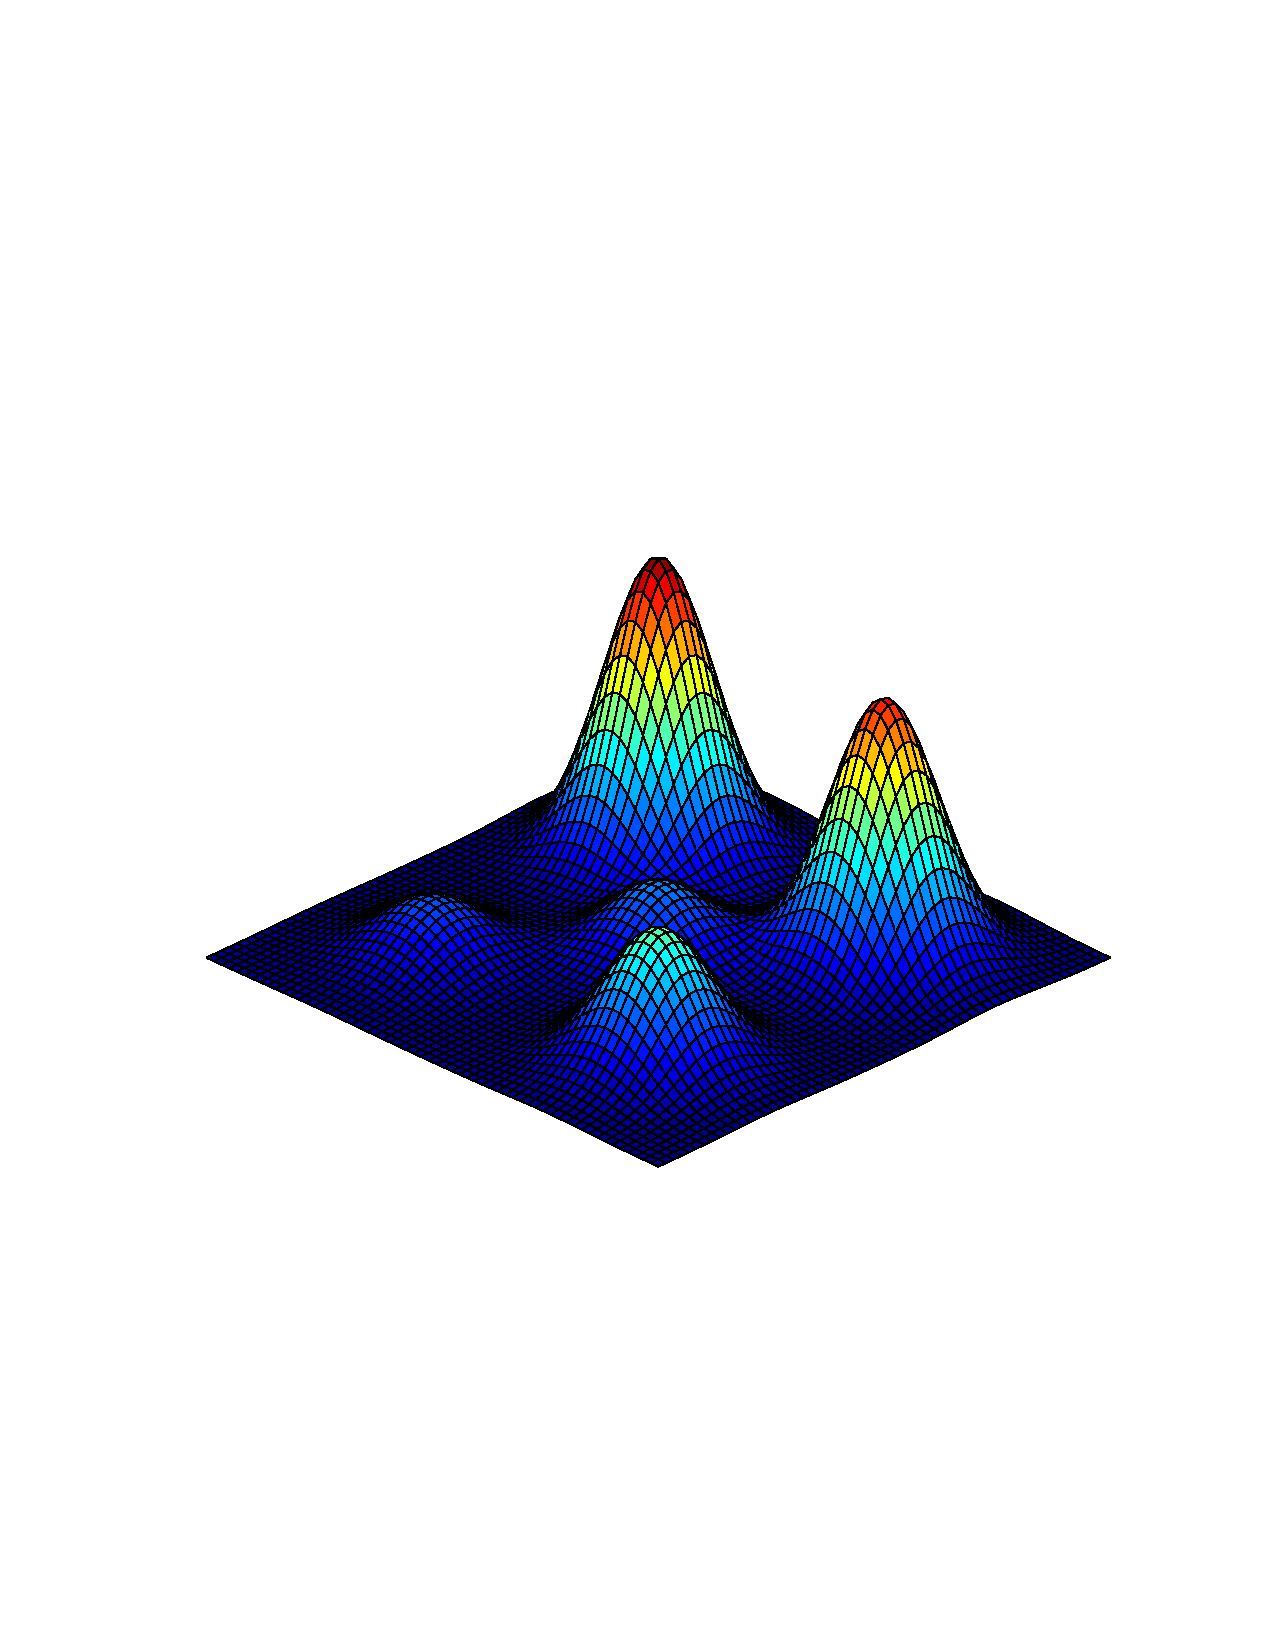
\includegraphics[width=0.5\textwidth]{gaussian}
\caption{Multiple three-dimensional gaussian distributions...}
\label{fig:mog}
\end{figure}


This is the text beneath an included picture. Figure \ref{fig:mog} shows an example of how to include eps-figures in this document.

\subsubsection{Displaying two eps-figures side-by-side}
\begin{figure}[H]
 \centering
 \begin{subfigure}{0.49\textwidth}
    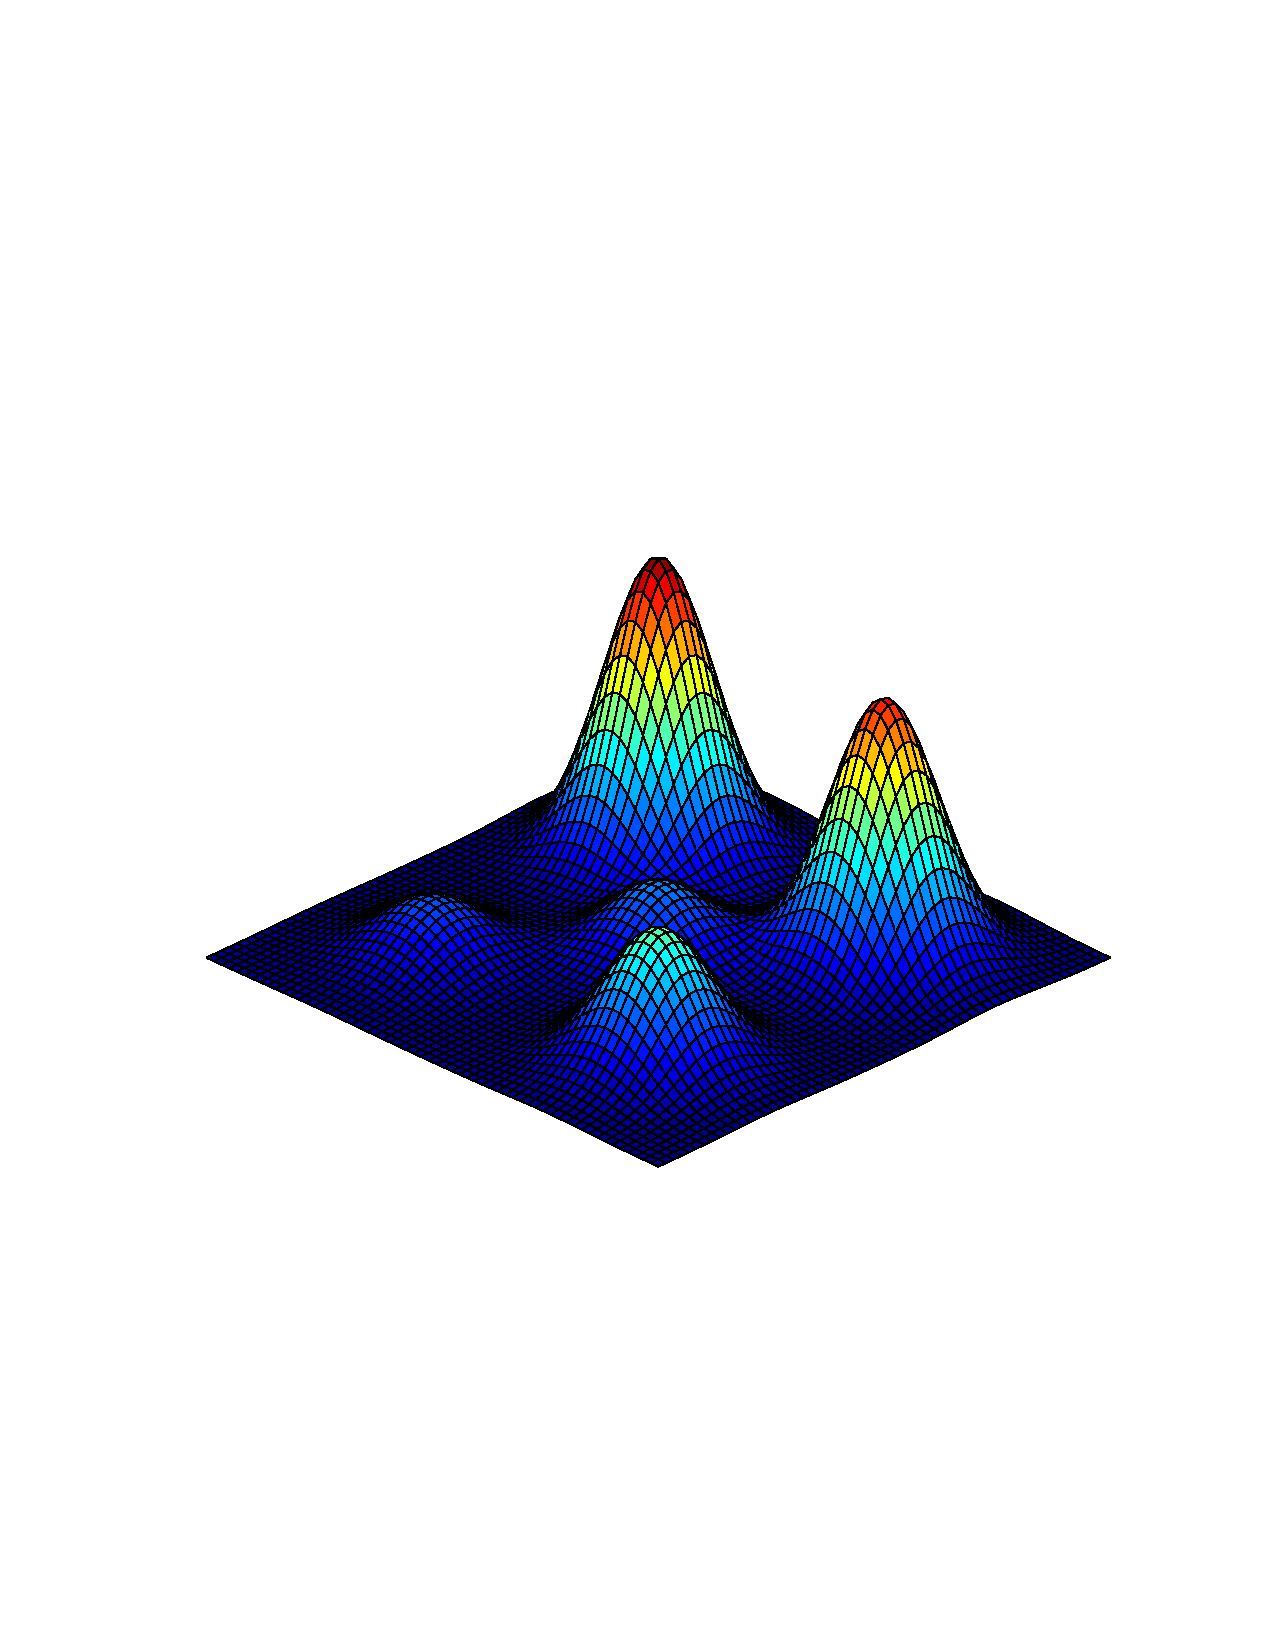
\includegraphics[width=\textwidth]{gaussian}
    \caption{Sub caption}
 \end{subfigure}
 \begin{subfigure}{0.49\textwidth}
    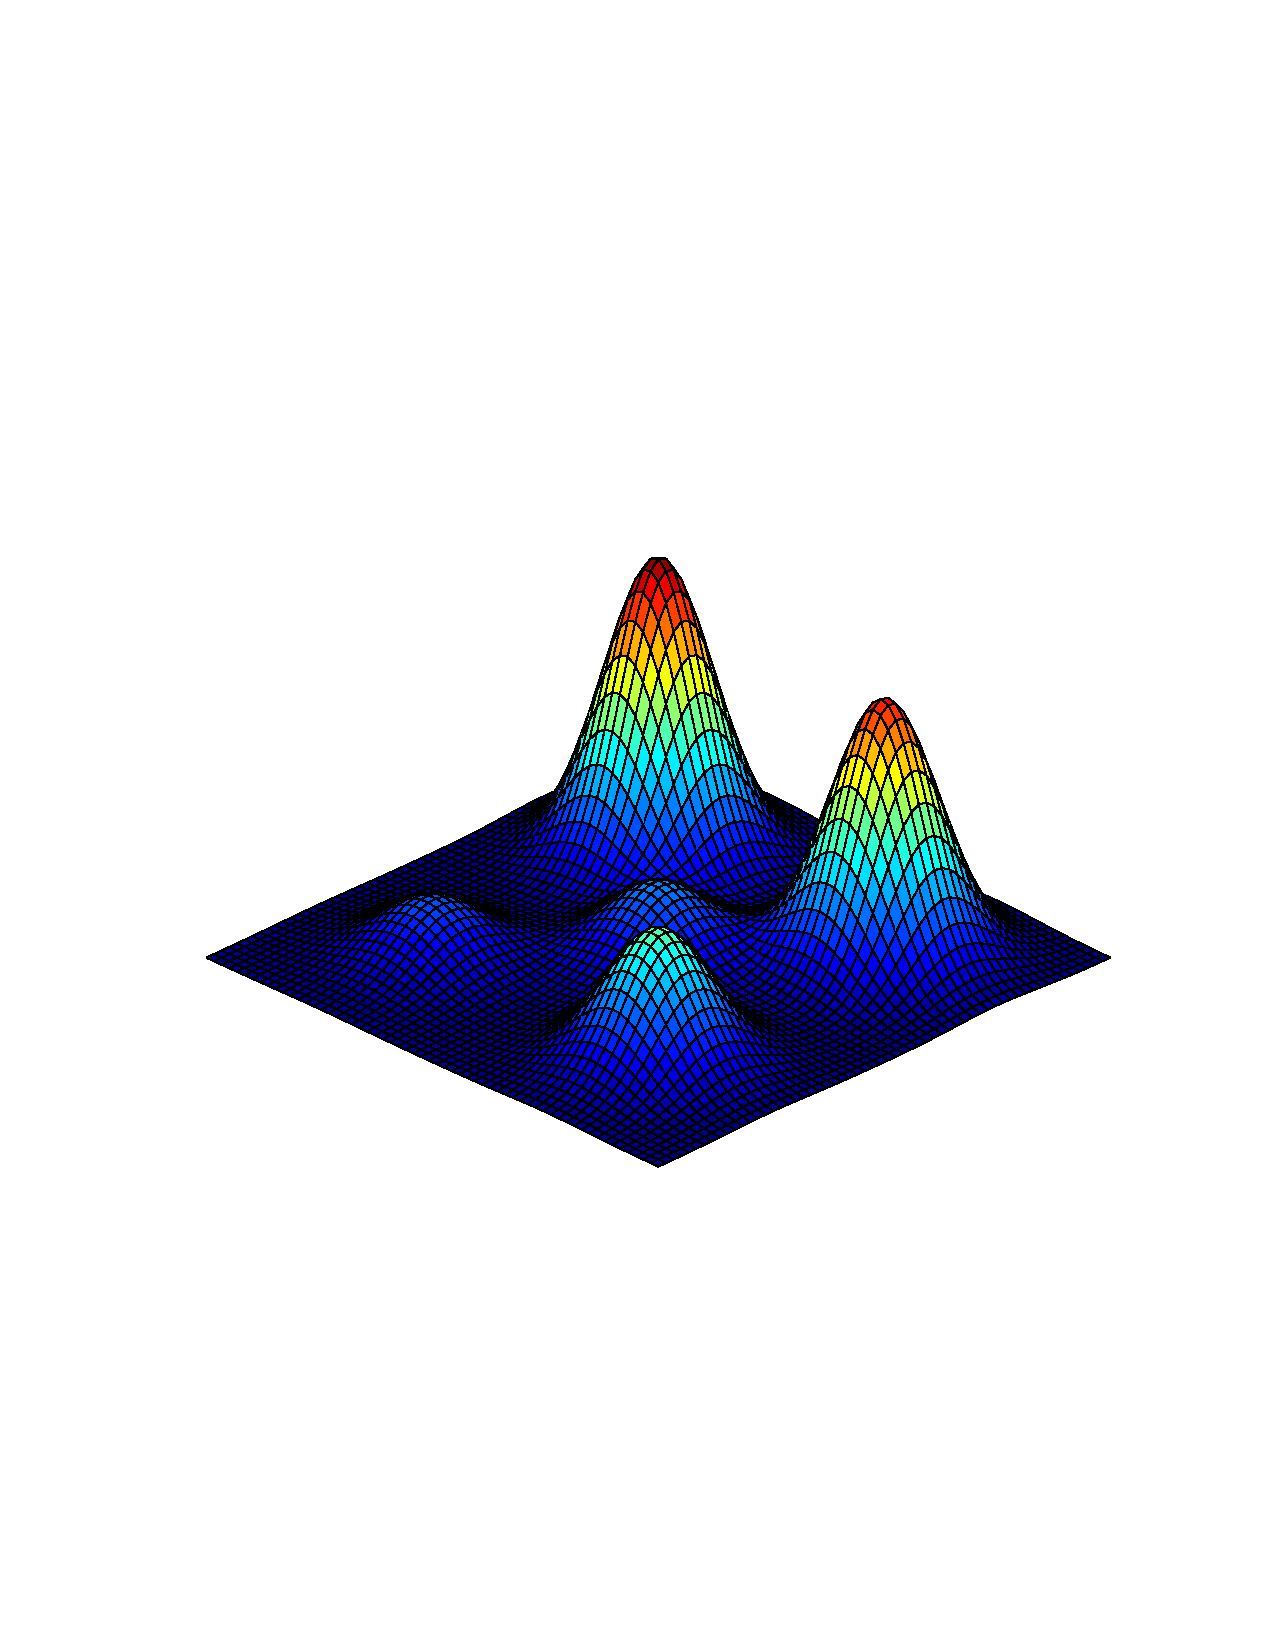
\includegraphics[width=\textwidth]{gaussian}
    \caption{Sub caption}
 \end{subfigure}
 \caption{Main caption}
\end{figure}

\subsection{Including tikz-figures}
\subsubsection{Two-dimensional figures}
Graphs can be included, like is shown in figure \ref{fig:sin}, using the input-method.
\tikzset{every picture/.style={scale=0.9}}
\begin{figure}[H]
	\centering
	% This file was created by matlab2tikz.
%
%The latest updates can be retrieved from
%  http://www.mathworks.com/matlabcentral/fileexchange/22022-matlab2tikz-matlab2tikz
%where you can also make suggestions and rate matlab2tikz.
%
\definecolor{mycolor1}{rgb}{0.00000,0.44700,0.74100}%
%
\begin{tikzpicture}

\begin{axis}[%
width=6.028in,
height=4.754in,
at={(1.011in,0.642in)},
scale only axis,
xmin=0,
xmax=6.28318530717959,
xtick={0,1.5707963267949,3.14159265358979,4.71238898038469,6.28318530717959},
xticklabels={{0},{$\text{1/2 }\pi$},{$\pi$},{$\text{3/2 }\pi$},{$\text{2}\pi$}},
ymin=-1.5,
ymax=1.5,
ytick={-1,  0,  1},
axis background/.style={fill=white}
]
\addplot [color=mycolor1, forget plot]
  table[row sep=crcr]{%
0	0\\
0.126933036508679	0.126592453573749\\
0.253866073017357	0.251147987181079\\
0.380799109526036	0.371662455660328\\
0.507732146034714	0.486196736100469\\
0.634665182543393	0.59290792905464\\
0.761598219052071	0.690079011482112\\
0.88853125556075	0.776146464291757\\
1.01546429206943	0.849725429949514\\
1.14239732857811	0.909631995354518\\
1.26933036508679	0.954902241444074\\
1.39626340159546	0.984807753012208\\
1.52319643810414	0.998867339183008\\
1.65012947461282	0.996854775951942\\
1.7770625111215	0.978802446214779\\
1.90399554763018	0.945000818714669\\
2.03092858413886	0.895993774291336\\
2.15786162064753	0.832569854634771\\
2.28479465715621	0.755749574354258\\
2.41172769366489	0.666769000516292\\
2.53866073017357	0.567059863862771\\
2.66559376668225	0.458226521727411\\
2.79252680319093	0.342020143325669\\
2.91945983969961	0.220310532786541\\
3.04639287620828	0.0950560433041829\\
3.17332591271696	-0.0317279334980679\\
3.30025894922564	-0.15800139597335\\
3.42719198573432	-0.281732556841429\\
3.554125022243	-0.400930535406613\\
3.68105805875168	-0.513677391573406\\
3.80799109526036	-0.618158986220605\\
3.93492413176903	-0.712694171378863\\
4.06185716827771	-0.795761840530832\\
4.18879020478639	-0.866025403784438\\
4.31572324129507	-0.922354294104581\\
4.44265627780375	-0.963842158559942\\
4.56958931431243	-0.989821441880933\\
4.69652235082111	-0.999874127673875\\
4.82345538732978	-0.993838464461254\\
4.95038842383846	-0.971811568323542\\
5.07732146034714	-0.934147860265107\\
5.20425449685582	-0.881453363447582\\
5.3311875333645	-0.814575952050336\\
5.45812056987318	-0.734591708657534\\
5.58505360638185	-0.64278760968654\\
5.71198664289053	-0.540640817455597\\
5.83891967939921	-0.429794912089172\\
5.96585271590789	-0.312033445698487\\
6.09278575241657	-0.189251244360411\\
6.21971878892525	-0.0634239196565654\\
6.34665182543393	0.0634239196565649\\
6.4735848619426	0.18925124436041\\
6.60051789845128	0.312033445698487\\
6.72745093495996	0.429794912089172\\
6.85438397146864	0.540640817455597\\
6.98131700797732	0.642787609686539\\
7.108250044486	0.734591708657533\\
7.23518308099467	0.814575952050335\\
7.36211611750335	0.881453363447582\\
7.48904915401203	0.934147860265107\\
7.61598219052071	0.971811568323542\\
7.74291522702939	0.993838464461254\\
7.86984826353807	0.999874127673875\\
7.99678130004675	0.989821441880933\\
8.12371433655542	0.963842158559942\\
8.2506473730641	0.922354294104582\\
8.37758040957278	0.866025403784439\\
8.50451344608146	0.795761840530832\\
8.63144648259014	0.712694171378863\\
8.75837951909882	0.618158986220606\\
8.88531255560749	0.513677391573407\\
9.01224559211617	0.400930535406613\\
9.13917862862485	0.28173255684143\\
9.26611166513353	0.158001395973351\\
9.39304470164221	0.031727933498067\\
9.51997773815089	-0.0950560433041828\\
9.64691077465957	-0.22031053278654\\
9.77384381116824	-0.342020143325668\\
9.90077684767692	-0.458226521727409\\
10.0277098841856	-0.567059863862771\\
10.1546429206943	-0.666769000516291\\
10.281575957203	-0.755749574354258\\
10.4085089937116	-0.832569854634771\\
10.5354420302203	-0.895993774291336\\
10.662375066729	-0.945000818714668\\
10.7893081032377	-0.978802446214779\\
10.9162411397464	-0.996854775951942\\
11.043174176255	-0.998867339183008\\
11.1701072127637	-0.984807753012208\\
11.2970402492724	-0.954902241444074\\
11.4239732857811	-0.909631995354518\\
11.5509063222897	-0.849725429949514\\
11.6778393587984	-0.776146464291757\\
11.8047723953071	-0.690079011482113\\
11.9317054318158	-0.59290792905464\\
12.0586384683245	-0.486196736100469\\
12.1855715048331	-0.371662455660328\\
12.3125045413418	-0.251147987181081\\
12.4394375778505	-0.126592453573751\\
12.5663706143592	-4.89858719658941e-16\\
};
\end{axis}
\end{tikzpicture}%
	\caption{A sine wave}
	\label{fig:sin}
\end{figure}

As figure \ref{fig:sin} was a little big, we now try to scale this output somehow:

\tikzset{every picture/.style={scale=0.6}}
\begin{figure}[H]
	\centering
	% This file was created by matlab2tikz.
%
%The latest updates can be retrieved from
%  http://www.mathworks.com/matlabcentral/fileexchange/22022-matlab2tikz-matlab2tikz
%where you can also make suggestions and rate matlab2tikz.
%
\definecolor{mycolor1}{rgb}{0.00000,0.44700,0.74100}%
%
\begin{tikzpicture}

\begin{axis}[%
width=6.028in,
height=4.754in,
at={(1.011in,0.642in)},
scale only axis,
xmin=0,
xmax=6.28318530717959,
xtick={0,1.5707963267949,3.14159265358979,4.71238898038469,6.28318530717959},
xticklabels={{0},{$\text{1/2 }\pi$},{$\pi$},{$\text{3/2 }\pi$},{$\text{2}\pi$}},
ymin=-1.5,
ymax=1.5,
ytick={-1,  0,  1},
axis background/.style={fill=white}
]
\addplot [color=mycolor1, forget plot]
  table[row sep=crcr]{%
0	0\\
0.126933036508679	0.126592453573749\\
0.253866073017357	0.251147987181079\\
0.380799109526036	0.371662455660328\\
0.507732146034714	0.486196736100469\\
0.634665182543393	0.59290792905464\\
0.761598219052071	0.690079011482112\\
0.88853125556075	0.776146464291757\\
1.01546429206943	0.849725429949514\\
1.14239732857811	0.909631995354518\\
1.26933036508679	0.954902241444074\\
1.39626340159546	0.984807753012208\\
1.52319643810414	0.998867339183008\\
1.65012947461282	0.996854775951942\\
1.7770625111215	0.978802446214779\\
1.90399554763018	0.945000818714669\\
2.03092858413886	0.895993774291336\\
2.15786162064753	0.832569854634771\\
2.28479465715621	0.755749574354258\\
2.41172769366489	0.666769000516292\\
2.53866073017357	0.567059863862771\\
2.66559376668225	0.458226521727411\\
2.79252680319093	0.342020143325669\\
2.91945983969961	0.220310532786541\\
3.04639287620828	0.0950560433041829\\
3.17332591271696	-0.0317279334980679\\
3.30025894922564	-0.15800139597335\\
3.42719198573432	-0.281732556841429\\
3.554125022243	-0.400930535406613\\
3.68105805875168	-0.513677391573406\\
3.80799109526036	-0.618158986220605\\
3.93492413176903	-0.712694171378863\\
4.06185716827771	-0.795761840530832\\
4.18879020478639	-0.866025403784438\\
4.31572324129507	-0.922354294104581\\
4.44265627780375	-0.963842158559942\\
4.56958931431243	-0.989821441880933\\
4.69652235082111	-0.999874127673875\\
4.82345538732978	-0.993838464461254\\
4.95038842383846	-0.971811568323542\\
5.07732146034714	-0.934147860265107\\
5.20425449685582	-0.881453363447582\\
5.3311875333645	-0.814575952050336\\
5.45812056987318	-0.734591708657534\\
5.58505360638185	-0.64278760968654\\
5.71198664289053	-0.540640817455597\\
5.83891967939921	-0.429794912089172\\
5.96585271590789	-0.312033445698487\\
6.09278575241657	-0.189251244360411\\
6.21971878892525	-0.0634239196565654\\
6.34665182543393	0.0634239196565649\\
6.4735848619426	0.18925124436041\\
6.60051789845128	0.312033445698487\\
6.72745093495996	0.429794912089172\\
6.85438397146864	0.540640817455597\\
6.98131700797732	0.642787609686539\\
7.108250044486	0.734591708657533\\
7.23518308099467	0.814575952050335\\
7.36211611750335	0.881453363447582\\
7.48904915401203	0.934147860265107\\
7.61598219052071	0.971811568323542\\
7.74291522702939	0.993838464461254\\
7.86984826353807	0.999874127673875\\
7.99678130004675	0.989821441880933\\
8.12371433655542	0.963842158559942\\
8.2506473730641	0.922354294104582\\
8.37758040957278	0.866025403784439\\
8.50451344608146	0.795761840530832\\
8.63144648259014	0.712694171378863\\
8.75837951909882	0.618158986220606\\
8.88531255560749	0.513677391573407\\
9.01224559211617	0.400930535406613\\
9.13917862862485	0.28173255684143\\
9.26611166513353	0.158001395973351\\
9.39304470164221	0.031727933498067\\
9.51997773815089	-0.0950560433041828\\
9.64691077465957	-0.22031053278654\\
9.77384381116824	-0.342020143325668\\
9.90077684767692	-0.458226521727409\\
10.0277098841856	-0.567059863862771\\
10.1546429206943	-0.666769000516291\\
10.281575957203	-0.755749574354258\\
10.4085089937116	-0.832569854634771\\
10.5354420302203	-0.895993774291336\\
10.662375066729	-0.945000818714668\\
10.7893081032377	-0.978802446214779\\
10.9162411397464	-0.996854775951942\\
11.043174176255	-0.998867339183008\\
11.1701072127637	-0.984807753012208\\
11.2970402492724	-0.954902241444074\\
11.4239732857811	-0.909631995354518\\
11.5509063222897	-0.849725429949514\\
11.6778393587984	-0.776146464291757\\
11.8047723953071	-0.690079011482113\\
11.9317054318158	-0.59290792905464\\
12.0586384683245	-0.486196736100469\\
12.1855715048331	-0.371662455660328\\
12.3125045413418	-0.251147987181081\\
12.4394375778505	-0.126592453573751\\
12.5663706143592	-4.89858719658941e-16\\
};
\end{axis}
\end{tikzpicture}%
	\caption{A second sine wave}
	\label{fig:sin2}
\end{figure}

We can also display more than one lineplot in one row:

\tikzset{every picture/.style={scale=0.5}}
\begin{figure}[H]
	\centering
	\begin{subfigure}{0.49\textwidth}
		\includestandalone[width=\textwidth]{plots/sin-tikz}
		\caption{A sine wave}
	\end{subfigure}
	\begin{subfigure}{0.49\textwidth}
		\includestandalone[width=\textwidth]{plots/cos-tikz}
		\caption{A cosine wave}
	\end{subfigure}
	\caption{Sine and cosine waves}
	\label{fig:sin}
\end{figure}

\subsubsection{Three-dimensional figures}
\tikzset{every picture/.style={scale=1}}
\begin{figure}[H]
	\centering
	% This file was created by matlab2tikz.
%
%The latest updates can be retrieved from
%  http://www.mathworks.com/matlabcentral/fileexchange/22022-matlab2tikz-matlab2tikz
%where you can also make suggestions and rate matlab2tikz.
%
\begin{tikzpicture}

\begin{axis}[%
xmin=-4,
xmax=4,
tick align=outside,
ymin=-4,
ymax=4,
zmin=0.00010706418061697,
zmax=1.59228132227989,
view={-45}{45},
axis line style={draw=none},
ticks=none,
axis x line*=bottom,
axis y line*=left,
axis z line*=left
]

\addplot3[%
surf,
shader=flat corner, draw=black, z buffer=sort, colormap/jet, mesh/rows=60]
table[row sep=crcr, point meta=\thisrow{c}] {%
%
x	y	z	c\\
-4	-4	0.000240894406381853	0.000240894406381853\\
-4	-3.86440677966102	0.000406809920133187	0.000406809920133187\\
-4	-3.72881355932203	0.000662196517972816	0.000662196517972816\\
-4	-3.59322033898305	0.00103899340249576	0.00103899340249576\\
-4	-3.45762711864407	0.00157133659858499	0.00157133659858499\\
-4	-3.32203389830508	0.002290636628699	0.002290636628699\\
-4	-3.1864406779661	0.00321864971646203	0.00321864971646203\\
-4	-3.05084745762712	0.00435935029968579	0.00435935029968579\\
-4	-2.91525423728814	0.00569115430686962	0.00569115430686962\\
-4	-2.77966101694915	0.0071615906361871	0.0071615906361871\\
-4	-2.64406779661017	0.00868658680238613	0.00868658680238613\\
-4	-2.50847457627119	0.0101559224202182	0.0101559224202182\\
-4	-2.3728813559322	0.011445114087472	0.011445114087472\\
-4	-2.23728813559322	0.0124322982404674	0.0124322982404674\\
-4	-2.10169491525424	0.0130170705940178	0.0130170705940178\\
-4	-1.96610169491525	0.0131372860783609	0.0131372860783609\\
-4	-1.83050847457627	0.0127799348448428	0.0127799348448428\\
-4	-1.69491525423729	0.0119834615453927	0.0119834615453927\\
-4	-1.5593220338983	0.0108309567988372	0.0108309567988372\\
-4	-1.42372881355932	0.00943589075238768	0.00943589075238768\\
-4	-1.28813559322034	0.00792378049543821	0.00792378049543821\\
-4	-1.15254237288136	0.00641388285102141	0.00641388285102141\\
-4	-1.01694915254237	0.00500455156716988	0.00500455156716988\\
-4	-0.88135593220339	0.00376455424208149	0.00376455424208149\\
-4	-0.745762711864407	0.00273092578155718	0.00273092578155718\\
-4	-0.610169491525424	0.0019123960842761	0.0019123960842761\\
-4	-0.474576271186441	0.00129646378824614	0.00129646378824614\\
-4	-0.338983050847458	0.000857925813243877	0.000857925813243877\\
-4	-0.203389830508474	0.000566996259590799	0.000566996259590799\\
-4	-0.0677966101694913	0.000395792909851026	0.000395792909851026\\
-4	0.0677966101694913	0.000322651022997548	0.000322651022997548\\
-4	0.203389830508475	0.000334239923533917	0.000334239923533917\\
-4	0.338983050847458	0.00042573217033684	0.00042573217033684\\
-4	0.47457627118644	0.000599347682502313	0.000599347682502313\\
-4	0.610169491525424	0.000861574564579196	0.000861574564579196\\
-4	0.745762711864407	0.0012193720856427	0.0012193720856427\\
-4	0.88135593220339	0.00167576383591249	0.00167576383591249\\
-4	1.01694915254237	0.00222543023837267	0.00222543023837267\\
-4	1.15254237288136	0.0028511307581813	0.0028511307581813\\
-4	1.28813559322034	0.00352189773692076	0.00352189773692076\\
-4	1.42372881355932	0.00419381814718419	0.00419381814718419\\
-4	1.55932203389831	0.00481379399399683	0.00481379399399683\\
-4	1.69491525423729	0.00532599674365331	0.00532599674365331\\
-4	1.83050847457627	0.00567997639490969	0.00567997639490969\\
-4	1.96610169491525	0.0058387958911201	0.0058387958911201\\
-4	2.10169491525424	0.00578536553055326	0.00578536553055326\\
-4	2.23728813559322	0.00552546622000061	0.00552546622000061\\
-4	2.3728813559322	0.00508671751400214	0.00508671751400214\\
-4	2.50847457627119	0.00451374335971974	0.00451374335971974\\
-4	2.64406779661017	0.00386070527299022	0.00386070527299022\\
-4	2.77966101694915	0.00318292918390204	0.00318292918390204\\
-4	2.91525423728814	0.00252940191958541	0.00252940191958541\\
-4	3.05084745762712	0.00193748902443343	0.00193748902443343\\
-4	3.1864406779661	0.00143051098608754	0.00143051098608754\\
-4	3.32203389830508	0.00101806072427341	0.00101806072427341\\
-4	3.45762711864407	0.000698371821754849	0.000698371821754849\\
-4	3.59322033898305	0.000461774845615573	0.000461774845615573\\
-4	3.72881355932203	0.000294309563566372	0.000294309563566372\\
-4	3.86440677966102	0.000180804408956255	0.000180804408956255\\
-4	4	0.00010706418061697	0.00010706418061697\\
-3.86440677966102	-4	0.000406809920133202	0.000406809920133202\\
-3.86440677966102	-3.86440677966102	0.000686999393660653	0.000686999393660653\\
-3.86440677966102	-3.72881355932203	0.00111828297154378	0.00111828297154378\\
-3.86440677966102	-3.59322033898305	0.00175459791475743	0.00175459791475743\\
-3.86440677966102	-3.45762711864407	0.00265359136332252	0.00265359136332252\\
-3.86440677966102	-3.32203389830508	0.00386830777089914	0.00386830777089914\\
-3.86440677966102	-3.1864406779661	0.00543548791459898	0.00543548791459898\\
-3.86440677966102	-3.05084745762712	0.00736184361874751	0.00736184361874751\\
-3.86440677966102	-2.91525423728814	0.00961092482993479	0.00961092482993479\\
-3.86440677966102	-2.77966101694915	0.0120941210891849	0.0120941210891849\\
-3.86440677966102	-2.64406779661017	0.0146694551709669	0.0146694551709669\\
-3.86440677966102	-2.50847457627119	0.017150792643851	0.017150792643851\\
-3.86440677966102	-2.3728813559322	0.0193279124445809	0.0193279124445809\\
-3.86440677966102	-2.23728813559322	0.0209950177685511	0.0209950177685511\\
-3.86440677966102	-2.10169491525424	0.0219825511389007	0.0219825511389007\\
-3.86440677966102	-1.96610169491525	0.0221855652691735	0.0221855652691735\\
-3.86440677966102	-1.83050847457627	0.0215820898982454	0.0215820898982454\\
-3.86440677966102	-1.69491525423729	0.0202370484685822	0.0202370484685822\\
-3.86440677966102	-1.5593220338983	0.0182907602235547	0.0182907602235547\\
-3.86440677966102	-1.42372881355932	0.0159348477758091	0.0159348477758091\\
-3.86440677966102	-1.28813559322034	0.0133812779683647	0.0133812779683647\\
-3.86440677966102	-1.15254237288136	0.0108314455843995	0.0108314455843995\\
-3.86440677966102	-1.01694915254237	0.00845144530099282	0.00845144530099282\\
-3.86440677966102	-0.88135593220339	0.00635740813422297	0.00635740813422297\\
-3.86440677966102	-0.745762711864407	0.00461187645182233	0.00461187645182233\\
-3.86440677966102	-0.610169491525424	0.00322959247244462	0.00322959247244462\\
-3.86440677966102	-0.474576271186441	0.00218944406951474	0.00218944406951474\\
-3.86440677966102	-0.338983050847458	0.00144886907337665	0.00144886907337665\\
-3.86440677966102	-0.203389830508474	0.000957566117969549	0.000957566117969549\\
-3.86440677966102	-0.0677966101694913	0.000668448784578175	0.000668448784578175\\
-3.86440677966102	0.0677966101694913	0.000544930577594	0.000544930577594\\
-3.86440677966102	0.203389830508475	0.000564499346920215	0.000564499346920215\\
-3.86440677966102	0.338983050847458	0.000719002971497464	0.000719002971497464\\
-3.86440677966102	0.47457627118644	0.00101219071790565	0.00101219071790565\\
-3.86440677966102	0.610169491525424	0.00145501984987389	0.00145501984987389\\
-3.86440677966102	0.745762711864407	0.00205924333950357	0.00205924333950357\\
-3.86440677966102	0.88135593220339	0.00282996774630147	0.00282996774630147\\
-3.86440677966102	1.01694915254237	0.00375821002512177	0.00375821002512177\\
-3.86440677966102	1.15254237288136	0.00481485551039315	0.00481485551039315\\
-3.86440677966102	1.28813559322034	0.00594760775452637	0.00594760775452637\\
-3.86440677966102	1.42372881355932	0.0070823087324468	0.0070823087324468\\
-3.86440677966102	1.55932203389831	0.00812928924216433	0.00812928924216433\\
-3.86440677966102	1.69491525423729	0.00899426884193092	0.00899426884193092\\
-3.86440677966102	1.83050847457627	0.00959205005753566	0.00959205005753566\\
-3.86440677966102	1.96610169491525	0.00986025537628656	0.00986025537628656\\
-3.86440677966102	2.10169491525424	0.00977002448277358	0.00977002448277358\\
-3.86440677966102	2.23728813559322	0.00933111977781463	0.00933111977781463\\
-3.86440677966102	2.3728813559322	0.00859018365693499	0.00859018365693499\\
-3.86440677966102	2.50847457627119	0.00762257466893706	0.00762257466893706\\
-3.86440677966102	2.64406779661017	0.00651975792808413	0.00651975792808413\\
-3.86440677966102	2.77966101694915	0.00537516496261161	0.00537516496261161\\
-3.86440677966102	2.91525423728814	0.00427152216197213	0.00427152216197213\\
-3.86440677966102	3.05084745762712	0.00327193050394308	0.00327193050394308\\
-3.86440677966102	3.1864406779661	0.00241577240934721	0.00241577240934721\\
-3.86440677966102	3.32203389830508	0.00171924789935387	0.00171924789935387\\
-3.86440677966102	3.45762711864407	0.00117937393972221	0.00117937393972221\\
-3.86440677966102	3.59322033898305	0.00077982129562726	0.00077982129562726\\
-3.86440677966102	3.72881355932203	0.000497014654085927	0.000497014654085927\\
-3.86440677966102	3.86440677966102	0.000305333063872918	0.000305333063872918\\
-3.86440677966102	4	0.000180804408956268	0.000180804408956268\\
-3.72881355932203	-4	0.000662196517972913	0.000662196517972913\\
-3.72881355932203	-3.86440677966102	0.00111828297154391	0.00111828297154391\\
-3.72881355932203	-3.72881355932203	0.00182031718808603	0.00182031718808603\\
-3.72881355932203	-3.59322033898305	0.00285609709157999	0.00285609709157999\\
-3.72881355932203	-3.45762711864407	0.00431945946818048	0.00431945946818048\\
-3.72881355932203	-3.32203389830508	0.0062967489495675	0.0062967489495675\\
-3.72881355932203	-3.1864406779661	0.00884777139082774	0.00884777139082774\\
-3.72881355932203	-3.05084745762712	0.0119834521589704	0.0119834521589704\\
-3.72881355932203	-2.91525423728814	0.0156444586388208	0.0156444586388208\\
-3.72881355932203	-2.77966101694915	0.0196865526233793	0.0196865526233793\\
-3.72881355932203	-2.64406779661017	0.0238786266287539	0.0238786266287539\\
-3.72881355932203	-2.50847457627119	0.0279176950264037	0.0279176950264037\\
-3.72881355932203	-2.3728813559322	0.0314615645041087	0.0314615645041087\\
-3.72881355932203	-2.23728813559322	0.0341752434968058	0.0341752434968058\\
-3.72881355932203	-2.10169491525424	0.0357827300909909	0.0357827300909909\\
-3.72881355932203	-1.96610169491525	0.0361131935233071	0.0361131935233071\\
-3.72881355932203	-1.83050847457627	0.0351308713322192	0.0351308713322192\\
-3.72881355932203	-1.69491525423729	0.0329414448432482	0.0329414448432482\\
-3.72881355932203	-1.5593220338983	0.0297733231117895	0.0297733231117895\\
-3.72881355932203	-1.42372881355932	0.0259384257379667	0.0259384257379667\\
-3.72881355932203	-1.28813559322034	0.0217817881766835	0.0217817881766835\\
-3.72881355932203	-1.15254237288136	0.0176312367740749	0.0176312367740749\\
-3.72881355932203	-1.01694915254237	0.0137571368853781	0.0137571368853781\\
-3.72881355932203	-0.88135593220339	0.0103485237670714	0.0103485237670714\\
-3.72881355932203	-0.745762711864407	0.00750720184898123	0.00750720184898123\\
-3.72881355932203	-0.610169491525424	0.00525716713841343	0.00525716713841343\\
-3.72881355932203	-0.474576271186441	0.00356405242757514	0.00356405242757514\\
-3.72881355932203	-0.338983050847458	0.0023585744646337	0.0023585744646337\\
-3.72881355932203	-0.203389830508474	0.00155885238355114	0.00155885238355114\\
-3.72881355932203	-0.0677966101694913	0.00108823884338998	0.00108823884338998\\
-3.72881355932203	0.0677966101694913	0.000887178538512814	0.000887178538512814\\
-3.72881355932203	0.203389830508475	0.000919026670776757	0.000919026670776757\\
-3.72881355932203	0.338983050847458	0.00117051397908811	0.00117051397908811\\
-3.72881355932203	0.47457627118644	0.00164774451175089	0.00164774451175089\\
-3.72881355932203	0.610169491525424	0.00236855564353913	0.00236855564353913\\
-3.72881355932203	0.745762711864407	0.00335208007111956	0.00335208007111956\\
-3.72881355932203	0.88135593220339	0.00460663148132596	0.00460663148132596\\
-3.72881355932203	1.01694915254237	0.00611758852674772	0.00611758852674772\\
-3.72881355932203	1.15254237288136	0.00783755967871634	0.00783755967871634\\
-3.72881355932203	1.28813559322034	0.00968141823088138	0.00968141823088138\\
-3.72881355932203	1.42372881355932	0.0115284513507614	0.0115284513507614\\
-3.72881355932203	1.55932203389831	0.013232697212155	0.013232697212155\\
-3.72881355932203	1.69491525423729	0.0146406877759849	0.0146406877759849\\
-3.72881355932203	1.83050847457627	0.0156137400143126	0.0156137400143126\\
-3.72881355932203	1.96610169491525	0.0160503167598276	0.0160503167598276\\
-3.72881355932203	2.10169491525424	0.0159034394766439	0.0159034394766439\\
-3.72881355932203	2.23728813559322	0.015188998931467	0.015188998931467\\
-3.72881355932203	2.3728813559322	0.0139829184288053	0.0139829184288053\\
-3.72881355932203	2.50847457627119	0.0124078648746611	0.0124078648746611\\
-3.72881355932203	2.64406779661017	0.0106127231452247	0.0106127231452247\\
-3.72881355932203	2.77966101694915	0.00874957903665748	0.00874957903665748\\
-3.72881355932203	2.91525423728814	0.00695309277062865	0.00695309277062865\\
-3.72881355932203	3.05084745762712	0.00532597875596783	0.00532597875596783\\
-3.72881355932203	3.1864406779661	0.00393234284832936	0.00393234284832936\\
-3.72881355932203	3.32203389830508	0.00279855509198064	0.00279855509198064\\
-3.72881355932203	3.45762711864407	0.0019197597649433	0.0019197597649433\\
-3.72881355932203	3.59322033898305	0.00126937648564892	0.00126937648564892\\
-3.72881355932203	3.72881355932203	0.000809029861557673	0.000809029861557673\\
-3.72881355932203	3.86440677966102	0.000497014654086027	0.000497014654086027\\
-3.72881355932203	4	0.000294309563566452	0.000294309563566452\\
-3.59322033898305	-4	0.00103899340249625	0.00103899340249625\\
-3.59322033898305	-3.86440677966102	0.00175459791475819	0.00175459791475819\\
-3.59322033898305	-3.72881355932203	0.00285609709158092	0.00285609709158092\\
-3.59322033898305	-3.59322033898305	0.00448124681275345	0.00448124681275345\\
-3.59322033898305	-3.45762711864407	0.00677727799759885	0.00677727799759885\\
-3.59322033898305	-3.32203389830508	0.00987966629590889	0.00987966629590889\\
-3.59322033898305	-3.1864406779661	0.0138822477355114	0.0138822477355114\\
-3.59322033898305	-3.05084745762712	0.0188021643403408	0.0188021643403408\\
-3.59322033898305	-2.91525423728814	0.024546322617412	0.024546322617412\\
-3.59322033898305	-2.77966101694915	0.0308884113068936	0.0308884113068936\\
-3.59322033898305	-2.64406779661017	0.0374658203491062	0.0374658203491062\\
-3.59322033898305	-2.50847457627119	0.0438031621463126	0.0438031621463126\\
-3.59322033898305	-2.3728813559322	0.0493635318868259	0.0493635318868259\\
-3.59322033898305	-2.23728813559322	0.0536213244667374	0.0536213244667374\\
-3.59322033898305	-2.10169491525424	0.0561434902995444	0.0561434902995444\\
-3.59322033898305	-1.96610169491525	0.056661994615278	0.056661994615278\\
-3.59322033898305	-1.83050847457627	0.0551207264353669	0.0551207264353669\\
-3.59322033898305	-1.69491525423729	0.0516855017765639	0.0516855017765639\\
-3.59322033898305	-1.5593220338983	0.0467146979137028	0.0467146979137028\\
-3.59322033898305	-1.42372881355932	0.0406977210941043	0.0406977210941043\\
-3.59322033898305	-1.28813559322034	0.0341759365600834	0.0341759365600834\\
-3.59322033898305	-1.15254237288136	0.0276637079141313	0.0276637079141313\\
-3.59322033898305	-1.01694915254237	0.0215852412287808	0.0215852412287808\\
-3.59322033898305	-0.88135593220339	0.0162371339303824	0.0162371339303824\\
-3.59322033898305	-0.745762711864407	0.011779116357115	0.011779116357115\\
-3.59322033898305	-0.610169491525424	0.00824883563424818	0.00824883563424818\\
-3.59322033898305	-0.474576271186441	0.00559236563474468	0.00559236563474468\\
-3.59322033898305	-0.338983050847458	0.00370099625918434	0.00370099625918434\\
-3.59322033898305	-0.203389830508474	0.00244625184580004	0.00244625184580004\\
-3.59322033898305	-0.0677966101694913	0.001707869005485	0.001707869005485\\
-3.59322033898305	0.0677966101694913	0.00139240324178497	0.00139240324178497\\
-3.59322033898305	0.203389830508475	0.00144235847540756	0.00144235847540756\\
-3.59322033898305	0.338983050847458	0.00183691668055531	0.00183691668055531\\
-3.59322033898305	0.47457627118644	0.00258565806748418	0.00258565806748418\\
-3.59322033898305	0.610169491525424	0.00371657337681315	0.00371657337681315\\
-3.59322033898305	0.745762711864407	0.00525968595179208	0.00525968595179208\\
-3.59322033898305	0.88135593220339	0.00722804366707794	0.00722804366707794\\
-3.59322033898305	1.01694915254237	0.0095987083388059	0.0095987083388059\\
-3.59322033898305	1.15254237288136	0.012297324051309	0.012297324051309\\
-3.59322033898305	1.28813559322034	0.015190327002109	0.015190327002109\\
-3.59322033898305	1.42372881355932	0.0180883175236951	0.0180883175236951\\
-3.59322033898305	1.55932203389831	0.0207622793858771	0.0207622793858771\\
-3.59322033898305	1.69491525423729	0.0229714186658289	0.0229714186658289\\
-3.59322033898305	1.83050847457627	0.0244981391464519	0.0244981391464519\\
-3.59322033898305	1.96610169491525	0.0251831268990621	0.0251831268990621\\
-3.59322033898305	2.10169491525424	0.024952671210213	0.024952671210213\\
-3.59322033898305	2.23728813559322	0.0238317041572535	0.0238317041572535\\
-3.59322033898305	2.3728813559322	0.0219393496945406	0.0219393496945406\\
-3.59322033898305	2.50847457627119	0.0194680731456958	0.0194680731456958\\
-3.59322033898305	2.64406779661017	0.0166514762339964	0.0166514762339964\\
-3.59322033898305	2.77966101694915	0.0137281830499537	0.0137281830499537\\
-3.59322033898305	2.91525423728814	0.0109094768318625	0.0109094768318625\\
-3.59322033898305	3.05084745762712	0.00835651753465311	0.00835651753465311\\
-3.59322033898305	3.1864406779661	0.00616988790387061	0.00616988790387061\\
-3.59322033898305	3.32203389830508	0.00439096280703006	0.00439096280703006\\
-3.59322033898305	3.45762711864407	0.00301212355801462	0.00301212355801462\\
-3.59322033898305	3.59322033898305	0.00199166525146815	0.00199166525146815\\
-3.59322033898305	3.72881355932203	0.00126937648564968	0.00126937648564968\\
-3.59322033898305	3.86440677966102	0.000779821295627881	0.000779821295627881\\
-3.59322033898305	4	0.000461774845615974	0.000461774845615974\\
-3.45762711864407	-4	0.00157133659858724	0.00157133659858724\\
-3.45762711864407	-3.86440677966102	0.00265359136332623	0.00265359136332623\\
-3.45762711864407	-3.72881355932203	0.00431945946818605	0.00431945946818605\\
-3.45762711864407	-3.59322033898305	0.00677727799760538	0.00677727799760538\\
-3.45762711864407	-3.45762711864407	0.0102497137490842	0.0102497137490842\\
-3.45762711864407	-3.32203389830508	0.0149416552714051	0.0149416552714051\\
-3.45762711864407	-3.1864406779661	0.0209950168372592	0.0209950168372592\\
-3.45762711864407	-3.05084745762712	0.0284357234497711	0.0284357234497711\\
-3.45762711864407	-2.91525423728814	0.037122983862075	0.037122983862075\\
-3.45762711864407	-2.77966101694915	0.0467145330568013	0.0467145330568013\\
-3.45762711864407	-2.64406779661017	0.0566619726271079	0.0566619726271079\\
-3.45762711864407	-2.50847457627119	0.0662463435347629	0.0662463435347629\\
-3.45762711864407	-2.3728813559322	0.0746556504555945	0.0746556504555945\\
-3.45762711864407	-2.23728813559322	0.0810949875740217	0.0810949875740217\\
-3.45762711864407	-2.10169491525424	0.0849094270652105	0.0849094270652105\\
-3.45762711864407	-1.96610169491525	0.0856936040483117	0.0856936040483117\\
-3.45762711864407	-1.83050847457627	0.0833626601132141	0.0833626601132141\\
-3.45762711864407	-1.69491525423729	0.0781673718085772	0.0781673718085772\\
-3.45762711864407	-1.5593220338983	0.0706497388332479	0.0706497388332479\\
-3.45762711864407	-1.42372881355932	0.0615499245305459	0.0615499245305459\\
-3.45762711864407	-1.28813559322034	0.0516866728264061	0.0516866728264061\\
-3.45762711864407	-1.15254237288136	0.0418378903805545	0.0418378903805545\\
-3.45762711864407	-1.01694915254237	0.0326451311986974	0.0326451311986974\\
-3.45762711864407	-0.88135593220339	0.0245569562971701	0.0245569562971701\\
-3.45762711864407	-0.745762711864407	0.0178149312088889	0.0178149312088889\\
-3.45762711864407	-0.610169491525424	0.0124759846483913	0.0124759846483913\\
-3.45762711864407	-0.474576271186441	0.00845855126832146	0.00845855126832146\\
-3.45762711864407	-0.338983050847458	0.00559821154372407	0.00559821154372407\\
-3.45762711864407	-0.203389830508474	0.00370065381257055	0.00370065381257055\\
-3.45762711864407	-0.0677966101694913	0.00258398848393541	0.00258398848393541\\
-3.45762711864407	0.0677966101694913	0.00210688930421658	0.00210688930421658\\
-3.45762711864407	0.203389830508475	0.00218240125190641	0.00218240125190641\\
-3.45762711864407	0.338983050847458	0.0027790440135821	0.0027790440135821\\
-3.45762711864407	0.47457627118644	0.00391131388455746	0.00391131388455746\\
-3.45762711864407	0.610169491525424	0.00562155271279447	0.00562155271279447\\
-3.45762711864407	0.745762711864407	0.00795517697713876	0.00795517697713876\\
-3.45762711864407	0.88135593220339	0.0109319292127012	0.0109319292127012\\
-3.45762711864407	1.01694915254237	0.0145171259837866	0.0145171259837866\\
-3.45762711864407	1.15254237288136	0.0185983189918551	0.0185983189918551\\
-3.45762711864407	1.28813559322034	0.022973513463779	0.022973513463779\\
-3.45762711864407	1.42372881355932	0.0273562682337199	0.0273562682337199\\
-3.45762711864407	1.55932203389831	0.0314002258397573	0.0314002258397573\\
-3.45762711864407	1.69491525423729	0.0347412157089981	0.0347412157089981\\
-3.45762711864407	1.83050847457627	0.0370501503021575	0.0370501503021575\\
-3.45762711864407	1.96610169491525	0.0380860862316859	0.0380860862316859\\
-3.45762711864407	2.10169491525424	0.0377375437275655	0.0377375437275655\\
-3.45762711864407	2.23728813559322	0.0360422273407271	0.0360422273407271\\
-3.45762711864407	2.3728813559322	0.0331802945407738	0.0331802945407738\\
-3.45762711864407	2.50847457627119	0.029442822086333	0.029442822086333\\
-3.45762711864407	2.64406779661017	0.0251831002853618	0.0251831002853618\\
-3.45762711864407	2.77966101694915	0.0207620153282559	0.0207620153282559\\
-3.45762711864407	2.91525423728814	0.0164991042311158	0.0164991042311158\\
-3.45762711864407	3.05084745762712	0.0126380994408306	0.0126380994408306\\
-3.45762711864407	3.1864406779661	0.00933111864997069	0.00933111864997069\\
-3.45762711864407	3.32203389830508	0.00664073569918149	0.00664073569918149\\
-3.45762711864407	3.45762711864407	0.00455542834209936	0.00455542834209936\\
-3.45762711864407	3.59322033898305	0.00301212355801994	0.00301212355801994\\
-3.45762711864407	3.72881355932203	0.00191975976494783	0.00191975976494783\\
-3.45762711864407	3.86440677966102	0.00117937393972523	0.00117937393972523\\
-3.45762711864407	4	0.000698371821756688	0.000698371821756688\\
-3.32203389830508	-4	0.00229063662870882	0.00229063662870882\\
-3.32203389830508	-3.86440677966102	0.00386830777091558	0.00386830777091558\\
-3.32203389830508	-3.72881355932203	0.00629674894959358	0.00629674894959358\\
-3.32203389830508	-3.59322033898305	0.00987966629594658	0.00987966629594658\\
-3.32203389830508	-3.45762711864407	0.0149416552714477	0.0149416552714477\\
-3.32203389830508	-3.32203389830508	0.0217813948663823	0.0217813948663823\\
-3.32203389830508	-3.1864406779661	0.0306057625013849	0.0306057625013849\\
-3.32203389830508	-3.05084745762712	0.0414525507338514	0.0414525507338514\\
-3.32203389830508	-2.91525423728814	0.05411651935563	0.05411651935563\\
-3.32203389830508	-2.77966101694915	0.0680987271980042	0.0680987271980042\\
-3.32203389830508	-2.64406779661017	0.0825997395748282	0.0825997395748282\\
-3.32203389830508	-2.50847457627119	0.0965714850393491	0.0965714850393491\\
-3.32203389830508	-2.3728813559322	0.108830267665267	0.108830267665267\\
-3.32203389830508	-2.23728813559322	0.118217304567324	0.118217304567324\\
-3.32203389830508	-2.10169491525424	0.123777868433718	0.123777868433718\\
-3.32203389830508	-1.96610169491525	0.124921036664237	0.124921036664237\\
-3.32203389830508	-1.83050847457627	0.12152311039333	0.12152311039333\\
-3.32203389830508	-1.69491525423729	0.113949668240008	0.113949668240008\\
-3.32203389830508	-1.5593220338983	0.102990824122939	0.102990824122939\\
-3.32203389830508	-1.42372881355932	0.0897255678638886	0.0897255678638886\\
-3.32203389830508	-1.28813559322034	0.0753474402868154	0.0753474402868154\\
-3.32203389830508	-1.15254237288136	0.0609904487749697	0.0609904487749697\\
-3.32203389830508	-1.01694915254237	0.0475898267757533	0.0475898267757533\\
-3.32203389830508	-0.88135593220339	0.0357994640968805	0.0357994640968805\\
-3.32203389830508	-0.745762711864407	0.0259714936927926	0.0259714936927926\\
-3.32203389830508	-0.610169491525424	0.0181888854508836	0.0181888854508836\\
-3.32203389830508	-0.474576271186441	0.0123327128551634	0.0123327128551634\\
-3.32203389830508	-0.338983050847458	0.0081632654894729	0.0081632654894729\\
-3.32203389830508	-0.203389830508474	0.00539725877320011	0.00539725877320011\\
-3.32203389830508	-0.0677966101694913	0.00376952188582425	0.00376952188582425\\
-3.32203389830508	0.0677966101694913	0.00307402427097591	0.00307402427097591\\
-3.32203389830508	0.203389830508475	0.00318400610045062	0.00318400610045062\\
-3.32203389830508	0.338983050847458	0.00405358688087179	0.00405358688087179\\
-3.32203389830508	0.47457627118644	0.00570391765073467	0.00570391765073467\\
-3.32203389830508	0.610169491525424	0.00819674699204703	0.00819674699204703\\
-3.32203389830508	0.745762711864407	0.0115983070626786	0.0115983070626786\\
-3.32203389830508	0.88135593220339	0.0159374013595755	0.0159374013595755\\
-3.32203389830508	1.01694915254237	0.0211634883436499	0.0211634883436499\\
-3.32203389830508	1.15254237288136	0.0271126574099467	0.0271126574099467\\
-3.32203389830508	1.28813559322034	0.0334904539402107	0.0334904539402107\\
-3.32203389830508	1.42372881355932	0.0398793149078437	0.0398793149078437\\
-3.32203389830508	1.55932203389831	0.045774329458205	0.045774329458205\\
-3.32203389830508	1.69491525423729	0.0506446170615753	0.0506446170615753\\
-3.32203389830508	1.83050847457627	0.0540104390652997	0.0540104390652997\\
-3.32203389830508	1.96610169491525	0.0555205503548157	0.0555205503548157\\
-3.32203389830508	2.10169491525424	0.055012434025361	0.055012434025361\\
-3.32203389830508	2.23728813559322	0.0525410497830322	0.0525410497830322\\
-3.32203389830508	2.3728813559322	0.0483690211572692	0.0483690211572692\\
-3.32203389830508	2.50847457627119	0.042920666774502	0.042920666774502\\
-3.32203389830508	2.64406779661017	0.0367109986956211	0.0367109986956211\\
-3.32203389830508	2.77966101694915	0.0302661025639606	0.0302661025639606\\
-3.32203389830508	2.91525423728814	0.024051787111268	0.024051787111268\\
-3.32203389830508	3.05084745762712	0.0184233562067007	0.0184233562067007\\
-3.32203389830508	3.1864406779661	0.0136025612511253	0.0136025612511253\\
-3.32203389830508	3.32203389830508	0.00968061999828932	0.00968061999828932\\
-3.32203389830508	3.45762711864407	0.00664073569921622	0.00664073569921622\\
-3.32203389830508	3.59322033898305	0.00439096280706077	0.00439096280706077\\
-3.32203389830508	3.72881355932203	0.00279855509200189	0.00279855509200189\\
-3.32203389830508	3.86440677966102	0.00171924789936726	0.00171924789936726\\
-3.32203389830508	4	0.00101806072428142	0.00101806072428142\\
-3.1864406779661	-4	0.00321864971650298	0.00321864971650298\\
-3.1864406779661	-3.86440677966102	0.00543548791466793	0.00543548791466793\\
-3.1864406779661	-3.72881355932203	0.00884777139093901	0.00884777139093901\\
-3.1864406779661	-3.59322033898305	0.0138822477356814	0.0138822477356814\\
-3.1864406779661	-3.45762711864407	0.0209950168374962	0.0209950168374962\\
-3.1864406779661	-3.32203389830508	0.0306057625016431	0.0306057625016431\\
-3.1864406779661	-3.1864406779661	0.0430051751210096	0.0430051751210096\\
-3.1864406779661	-3.05084745762712	0.0582463583778222	0.0582463583778222\\
-3.1864406779661	-2.91525423728814	0.0760409226390143	0.0760409226390143\\
-3.1864406779661	-2.77966101694915	0.0956877894830194	0.0956877894830194\\
-3.1864406779661	-2.64406779661017	0.116063647407061	0.116063647407061\\
-3.1864406779661	-2.50847457627119	0.135695817722827	0.135695817722827\\
-3.1864406779661	-2.3728813559322	0.152921052222245	0.152921052222245\\
-3.1864406779661	-2.23728813559322	0.166111110253141	0.166111110253141\\
-3.1864406779661	-2.10169491525424	0.17392447840235	0.17392447840235\\
-3.1864406779661	-1.96610169491525	0.175530839876129	0.175530839876129\\
-3.1864406779661	-1.83050847457627	0.170756392401545	0.170756392401545\\
-3.1864406779661	-1.69491525423729	0.160114836677124	0.160114836677124\\
-3.1864406779661	-1.5593220338983	0.144716404284598	0.144716404284598\\
-3.1864406779661	-1.42372881355932	0.126077236524607	0.126077236524607\\
-3.1864406779661	-1.28813559322034	0.105874432000457	0.105874432000457\\
-3.1864406779661	-1.15254237288136	0.0857014311505715	0.0857014311505715\\
-3.1864406779661	-1.01694915254237	0.06687236073661	0.06687236073661\\
-3.1864406779661	-0.88135593220339	0.0503060087596476	0.0503060087596476\\
-3.1864406779661	-0.745762711864407	0.0364971390154846	0.0364971390154846\\
-3.1864406779661	-0.610169491525424	0.0255622900647434	0.0255622900647434\\
-3.1864406779661	-0.474576271186441	0.0173342973699084	0.0173342973699084\\
-3.1864406779661	-0.338983050847458	0.0114762737669545	0.0114762737669545\\
-3.1864406779661	-0.203389830508474	0.00759010819059568	0.00759010819059568\\
-3.1864406779661	-0.0677966101694913	0.00530315468600819	0.00530315468600819\\
-3.1864406779661	0.0677966101694913	0.00432588785448017	0.00432588785448017\\
-3.1864406779661	0.203389830508475	0.00448019324525045	0.00448019324525045\\
-3.1864406779661	0.338983050847458	0.00570162766223445	0.00570162766223445\\
-3.1864406779661	0.47457627118644	0.00801995674820437	0.00801995674820437\\
-3.1864406779661	0.610169491525424	0.0115220039683119	0.0115220039683119\\
-3.1864406779661	0.745762711864407	0.0163008964158097	0.0163008964158097\\
-3.1864406779661	0.88135593220339	0.0223971637765784	0.0223971637765784\\
-3.1864406779661	1.01694915254237	0.0297398336407978	0.0297398336407978\\
-3.1864406779661	1.15254237288136	0.0380986196963832	0.0380986196963832\\
-3.1864406779661	1.28813559322034	0.0470597882821201	0.0470597882821201\\
-3.1864406779661	1.42372881355932	0.0560366085628267	0.0560366085628267\\
-3.1864406779661	1.55932203389831	0.0643196045567693	0.0643196045567693\\
-3.1864406779661	1.69491525423729	0.0711628036807831	0.0711628036807831\\
-3.1864406779661	1.83050847457627	0.0758920923836025	0.0758920923836025\\
-3.1864406779661	1.96610169491525	0.0780139082373324	0.0780139082373324\\
-3.1864406779661	2.10169491525424	0.0772998793121615	0.0772998793121615\\
-3.1864406779661	2.23728813559322	0.0738272202017467	0.0738272202017467\\
-3.1864406779661	2.3728813559322	0.0679649437559499	0.0679649437559499\\
-3.1864406779661	2.50847457627119	0.0603092685022295	0.0603092685022295\\
-3.1864406779661	2.64406779661017	0.0515838512950183	0.0515838512950183\\
-3.1864406779661	2.77966101694915	0.0425279102610573	0.0425279102610573\\
-3.1864406779661	2.91525423728814	0.0337959673811985	0.0337959673811985\\
-3.1864406779661	3.05084745762712	0.0258872711750595	0.0258872711750595\\
-3.1864406779661	3.1864406779661	0.0191134115018089	0.0191134115018089\\
-3.1864406779661	3.32203389830508	0.0136025612513357	0.0136025612513357\\
-3.1864406779661	3.45762711864407	0.0093311186501638	0.0093311186501638\\
-3.1864406779661	3.59322033898305	0.00616988790400919	0.00616988790400919\\
-3.1864406779661	3.72881355932203	0.00393234284842003	0.00393234284842003\\
-3.1864406779661	3.86440677966102	0.0024157724094034	0.0024157724094034\\
-3.1864406779661	4	0.00143051098612091	0.00143051098612091\\
-3.05084745762712	-4	0.00435935029985006	0.00435935029985006\\
-3.05084745762712	-3.86440677966102	0.00736184361902466	0.00736184361902466\\
-3.05084745762712	-3.72881355932203	0.0119834521594202	0.0119834521594202\\
-3.05084745762712	-3.59322033898305	0.0188021643410404	0.0188021643410404\\
-3.05084745762712	-3.45762711864407	0.0284357234508018	0.0284357234508018\\
-3.05084745762712	-3.32203389830508	0.0414525507352357	0.0414525507352357\\
-3.05084745762712	-3.1864406779661	0.058246358379276	0.058246358379276\\
-3.05084745762712	-3.05084745762712	0.0788890704331526	0.0788890704331526\\
-3.05084745762712	-2.91525423728814	0.10299009147029	0.10299009147029\\
-3.05084745762712	-2.77966101694915	0.129599879408771	0.129599879408771\\
-3.05084745762712	-2.64406779661017	0.157197019049099	0.157197019049099\\
-3.05084745762712	-2.50847457627119	0.18378691245855	0.18378691245855\\
-3.05084745762712	-2.3728813559322	0.207116855895579	0.207116855895579\\
-3.05084745762712	-2.23728813559322	0.224981563265864	0.224981563265864\\
-3.05084745762712	-2.10169491525424	0.235564097417766	0.235564097417766\\
-3.05084745762712	-1.96610169491525	0.237739893535175	0.237739893535175\\
-3.05084745762712	-1.83050847457627	0.231273579119095	0.231273579119095\\
-3.05084745762712	-1.69491525423729	0.216860944836328	0.216860944836328\\
-3.05084745762712	-1.5593220338983	0.19600572999929	0.19600572999929\\
-3.05084745762712	-1.42372881355932	0.170761440795616	0.170761440795616\\
-3.05084745762712	-1.28813559322034	0.143399579599542	0.143399579599542\\
-3.05084745762712	-1.15254237288136	0.116078328488528	0.116078328488528\\
-3.05084745762712	-1.01694915254237	0.0905775432812557	0.0905775432812557\\
-3.05084745762712	-0.88135593220339	0.0681416002677327	0.0681416002677327\\
-3.05084745762712	-0.745762711864407	0.0494405395133399	0.0494405395133399\\
-3.05084745762712	-0.610169491525424	0.0346320959738194	0.0346320959738194\\
-3.05084745762712	-0.474576271186441	0.023489728782841	0.023489728782841\\
-3.05084745762712	-0.338983050847458	0.015557012162048	0.015557012162048\\
-3.05084745762712	-0.203389830508474	0.010294606871742	0.010294606871742\\
-3.05084745762712	-0.0677966101694913	0.00719769367417461	0.00719769367417461\\
-3.05084745762712	0.0677966101694913	0.00587408010064036	0.00587408010064036\\
-3.05084745762712	0.203389830508475	0.0060825273235598	0.0060825273235598\\
-3.05084745762712	0.338983050847458	0.00773581152371952	0.00773581152371952\\
-3.05084745762712	0.47457627118644	0.010874353659414	0.010874353659414\\
-3.05084745762712	0.610169491525424	0.0156158839690756	0.0156158839690756\\
-3.05084745762712	0.745762711864407	0.0220866787489023	0.0220866787489023\\
-3.05084745762712	0.88135593220339	0.0303417641845875	0.0303417641845875\\
-3.05084745762712	1.01694915254237	0.0402851202724878	0.0402851202724878\\
-3.05084745762712	1.15254237288136	0.0516049161650599	0.0516049161650599\\
-3.05084745762712	1.28813559322034	0.0637408229154016	0.0637408229154016\\
-3.05084745762712	1.42372881355932	0.0758981722611437	0.0758981722611437\\
-3.05084745762712	1.55932203389831	0.0871160266394783	0.0871160266394783\\
-3.05084745762712	1.69491525423729	0.0963840039753224	0.0963840039753224\\
-3.05084745762712	1.83050847457627	0.102789043374392	0.102789043374392\\
-3.05084745762712	1.96610169491525	0.105662624357107	0.105662624357107\\
-3.05084745762712	2.10169491525424	0.10469540652696	0.10469540652696\\
-3.05084745762712	2.23728813559322	0.0999919436963738	0.0999919436963738\\
-3.05084745762712	2.3728813559322	0.0920520090258495	0.0920520090258495\\
-3.05084745762712	2.50847457627119	0.0816831096984842	0.0816831096984842\\
-3.05084745762712	2.64406779661017	0.0698653603871796	0.0698653603871796\\
-3.05084745762712	2.77966101694915	0.0575999552983686	0.0575999552983686\\
-3.05084745762712	2.91525423728814	0.0457733780930808	0.0457733780930808\\
-3.05084745762712	3.05084745762712	0.0350618109099921	0.0350618109099921\\
-3.05084745762712	3.1864406779661	0.0258872711762441	0.0258872711762441\\
-3.05084745762712	3.32203389830508	0.0184233562078286	0.0184233562078286\\
-3.05084745762712	3.45762711864407	0.0126380994416704	0.0126380994416704\\
-3.05084745762712	3.59322033898305	0.00835651753522317	0.00835651753522317\\
-3.05084745762712	3.72881355932203	0.00532597875633434	0.00532597875633434\\
-3.05084745762712	3.86440677966102	0.0032719305041689	0.0032719305041689\\
-3.05084745762712	4	0.00193748902456728	0.00193748902456728\\
-2.91525423728814	-4	0.00569115430750435	0.00569115430750435\\
-2.91525423728814	-3.86440677966102	0.00961092483100633	0.00961092483100633\\
-2.91525423728814	-3.72881355932203	0.0156444586405633	0.0156444586405633\\
-2.91525423728814	-3.59322033898305	0.024546322620138	0.024546322620138\\
-2.91525423728814	-3.45762711864407	0.0371229838661619	0.0371229838661619\\
-2.91525423728814	-3.32203389830508	0.0541165193614335	0.0541165193614335\\
-2.91525423728814	-3.1864406779661	0.0760409226465276	0.0760409226465276\\
-2.91525423728814	-3.05084745762712	0.102990091477896	0.102990091477896\\
-2.91525423728814	-2.91525423728814	0.134454102609359	0.134454102609359\\
-2.91525423728814	-2.77966101694915	0.169193326099041	0.169193326099041\\
-2.91525423728814	-2.64406779661017	0.205221550556431	0.205221550556431\\
-2.91525423728814	-2.50847457627119	0.239934825213513	0.239934825213513\\
-2.91525423728814	-2.3728813559322	0.27039224579403	0.27039224579403\\
-2.91525423728814	-2.23728813559322	0.293714819398438	0.293714819398438\\
-2.91525423728814	-2.10169491525424	0.30753055495846	0.30753055495846\\
-2.91525423728814	-1.96610169491525	0.310371370237828	0.310371370237828\\
-2.91525423728814	-1.83050847457627	0.30193004338554	0.30193004338554\\
-2.91525423728814	-1.69491525423729	0.283115006059437	0.283115006059437\\
-2.91525423728814	-1.5593220338983	0.255889482620306	0.255889482620306\\
-2.91525423728814	-1.42372881355932	0.222934423950395	0.222934423950395\\
-2.91525423728814	-1.28813559322034	0.187215364984201	0.187215364984201\\
-2.91525423728814	-1.15254237288136	0.151549870357776	0.151549870357776\\
-2.91525423728814	-1.01694915254237	0.118261546513797	0.118261546513797\\
-2.91525423728814	-0.88135593220339	0.0889748582198725	0.0889748582198725\\
-2.91525423728814	-0.745762711864407	0.0645643896550614	0.0645643896550614\\
-2.91525423728814	-0.610169491525424	0.0452358282179664	0.0452358282179664\\
-2.91525423728814	-0.474576271186441	0.0306931257876159	0.0306931257876159\\
-2.91525423728814	-0.338983050847458	0.0203400913571632	0.0203400913571632\\
-2.91525423728814	-0.203389830508474	0.0134723088358245	0.0134723088358245\\
-2.91525423728814	-0.0677966101694913	0.00943049546968636	0.00943049546968636\\
-2.91525423728814	0.0677966101694913	0.00770251112193273	0.00770251112193273\\
-2.91525423728814	0.203389830508475	0.00797341725879304	0.00797341725879304\\
-2.91525423728814	0.338983050847458	0.0101294735802652	0.0101294735802652\\
-2.91525423728814	0.47457627118644	0.014223688490962	0.014223688490962\\
-2.91525423728814	0.610169491525424	0.0204100653557578	0.0204100653557578\\
-2.91525423728814	0.745762711864407	0.0288537833295537	0.0288537833295537\\
-2.91525423728814	0.88135593220339	0.0396269772330375	0.0396269772330375\\
-2.91525423728814	1.01694915254237	0.0526045288559116	0.0526045288559116\\
-2.91525423728814	1.15254237288136	0.0673794980007292	0.0673794980007292\\
-2.91525423728814	1.28813559322034	0.0832204472347815	0.0832204472347815\\
-2.91525423728814	1.42372881355932	0.0990899375519827	0.0990899375519827\\
-2.91525423728814	1.55932203389831	0.11373341320582	0.11373341320582\\
-2.91525423728814	1.69491525423729	0.125831738317495	0.125831738317495\\
-2.91525423728814	1.83050847457627	0.134192819217906	0.134192819217906\\
-2.91525423728814	1.96610169491525	0.137943814040787	0.137943814040787\\
-2.91525423728814	2.10169491525424	0.136680803949564	0.136680803949564\\
-2.91525423728814	2.23728813559322	0.130540226325128	0.130540226325128\\
-2.91525423728814	2.3728813559322	0.12017449467453	0.12017449467453\\
-2.91525423728814	2.50847457627119	0.106637784035239	0.106637784035239\\
-2.91525423728814	2.64406779661017	0.0912096196964198	0.0912096196964198\\
-2.91525423728814	2.77966101694915	0.0751970537806648	0.0751970537806648\\
-2.91525423728814	2.91525423728814	0.059757388158383	0.059757388158383\\
-2.91525423728814	3.05084745762712	0.0457733780992778	0.0457733780992778\\
-2.91525423728814	3.1864406779661	0.0337959673873204	0.0337959673873204\\
-2.91525423728814	3.32203389830508	0.0240517871159968	0.0240517871159968\\
-2.91525423728814	3.45762711864407	0.0164991042344459	0.0164991042344459\\
-2.91525423728814	3.59322033898305	0.0109094768340837	0.0109094768340837\\
-2.91525423728814	3.72881355932203	0.00695309277204847	0.00695309277204847\\
-2.91525423728814	3.86440677966102	0.00427152216284523	0.00427152216284523\\
-2.91525423728814	4	0.00252940192010259	0.00252940192010259\\
-2.77966101694915	-4	0.00716159063855054	0.00716159063855054\\
-2.77966101694915	-3.86440677966102	0.0120941210931757	0.0120941210931757\\
-2.77966101694915	-3.72881355932203	0.0196865526298733	0.0196865526298733\\
-2.77966101694915	-3.59322033898305	0.0308884113170726	0.0308884113170726\\
-2.77966101694915	-3.45762711864407	0.0467145330721507	0.0467145330721507\\
-2.77966101694915	-3.32203389830508	0.0680987272201858	0.0680987272201858\\
-2.77966101694915	-3.1864406779661	0.0956877895133804	0.0956877895133804\\
-2.77966101694915	-3.05084745762712	0.129599879446657	0.129599879446657\\
-2.77966101694915	-2.91525423728814	0.169193326136007	0.169193326136007\\
-2.77966101694915	-2.77966101694915	0.212908218307907	0.212908218307907\\
-2.77966101694915	-2.64406779661017	0.258245171332214	0.258245171332214\\
-2.77966101694915	-2.50847457627119	0.301927461247344	0.301927461247344\\
-2.77966101694915	-2.3728813559322	0.340254361877186	0.340254361877186\\
-2.77966101694915	-2.23728813559322	0.36960307060744	0.36960307060744\\
-2.77966101694915	-2.10169491525424	0.38698880411548	0.38698880411548\\
-2.77966101694915	-1.96610169491525	0.390564261386598	0.390564261386598\\
-2.77966101694915	-1.83050847457627	0.379942968858908	0.379942968858908\\
-2.77966101694915	-1.69491525423729	0.356268230491688	0.356268230491688\\
-2.77966101694915	-1.5593220338983	0.322010697168727	0.322010697168727\\
-2.77966101694915	-1.42372881355932	0.280544193467241	0.280544193467241\\
-2.77966101694915	-1.28813559322034	0.235600632624806	0.235600632624806\\
-2.77966101694915	-1.15254237288136	0.190725661083157	0.190725661083157\\
-2.77966101694915	-1.01694915254237	0.148843230939718	0.148843230939718\\
-2.77966101694915	-0.88135593220339	0.111997361456149	0.111997361456149\\
-2.77966101694915	-0.745762711864407	0.0812882661665436	0.0812882661665436\\
-2.77966101694915	-0.610169491525424	0.0569742646961302	0.0569742646961302\\
-2.77966101694915	-0.474576271186441	0.0386821736049449	0.0386821736049449\\
-2.77966101694915	-0.338983050847458	0.0256610596477354	0.0256610596477354\\
-2.77966101694915	-0.203389830508474	0.0170238429761737	0.0170238429761737\\
-2.77966101694915	-0.0677966101694913	0.0119403839435587	0.0119403839435587\\
-2.77966101694915	0.0677966101694913	0.00976593639899136	0.00976593639899136\\
-2.77966101694915	0.203389830508475	0.0101041904324096	0.0101041904324096\\
-2.77966101694915	0.338983050847458	0.0128123016237669	0.0128123016237669\\
-2.77966101694915	0.47457627118644	0.017957490805202	0.017957490805202\\
-2.77966101694915	0.610169491525424	0.0257342137269667	0.0257342137269667\\
-2.77966101694915	0.745762711864407	0.03635103028217	0.03635103028217\\
-2.77966101694915	0.88135593220339	0.0498993576282096	0.0498993576282096\\
-2.77966101694915	1.01694915254237	0.0662222621702957	0.0662222621702957\\
-2.77966101694915	1.15254237288136	0.08480800058176	0.08480800058176\\
-2.77966101694915	1.28813559322034	0.10473631441401	0.10473631441401\\
-2.77966101694915	1.42372881355932	0.124701728975414	0.124701728975414\\
-2.77966101694915	1.55932203389831	0.143125444830931	0.143125444830931\\
-2.77966101694915	1.69491525423729	0.158347331620356	0.158347331620356\\
-2.77966101694915	1.83050847457627	0.168867101361611	0.168867101361611\\
-2.77966101694915	1.96610169491525	0.173586210239426	0.173586210239426\\
-2.77966101694915	2.10169491525424	0.171996219226512	0.171996219226512\\
-2.77966101694915	2.23728813559322	0.164268691447533	0.164268691447533\\
-2.77966101694915	2.3728813559322	0.1512245130265	0.1512245130265\\
-2.77966101694915	2.50847457627119	0.134190164167665	0.134190164167665\\
-2.77966101694915	2.64406779661017	0.114775721836207	0.114775721836207\\
-2.77966101694915	2.77966101694915	0.0946259180041575	0.0946259180041575\\
-2.77966101694915	2.91525423728814	0.0751970538107857	0.0751970538107857\\
-2.77966101694915	3.05084745762712	0.057599955329239	0.057599955329239\\
-2.77966101694915	3.1864406779661	0.0425279102857958	0.0425279102857958\\
-2.77966101694915	3.32203389830508	0.0302661025820346	0.0302661025820346\\
-2.77966101694915	3.45762711864407	0.0207620153407628	0.0207620153407628\\
-2.77966101694915	3.59322033898305	0.0137281830582477	0.0137281830582477\\
-2.77966101694915	3.72881355932203	0.00874957904194887	0.00874957904194887\\
-2.77966101694915	3.86440677966102	0.00537516496586337	0.00537516496586337\\
-2.77966101694915	4	0.0031829291858278	0.0031829291858278\\
-2.64406779661017	-4	0.00868658681086815	0.00868658681086815\\
-2.64406779661017	-3.86440677966102	0.0146694551852904	0.0146694551852904\\
-2.64406779661017	-3.72881355932203	0.0238786266520667	0.0238786266520667\\
-2.64406779661017	-3.59322033898305	0.037465820385672	0.037465820385672\\
-2.64406779661017	-3.45762711864407	0.0566619726823541	0.0566619726823541\\
-2.64406779661017	-3.32203389830508	0.0825997396551286	0.0825997396551286\\
-2.64406779661017	-3.1864406779661	0.116063647518915	0.116063647518915\\
-2.64406779661017	-3.05084745762712	0.157197019196671	0.157197019196671\\
-2.64406779661017	-2.91525423728814	0.205221550733932	0.205221550733932\\
-2.64406779661017	-2.77966101694915	0.258245171499153	0.258245171499153\\
-2.64406779661017	-2.64406779661017	0.313236293506464	0.313236293506464\\
-2.64406779661017	-2.50847457627119	0.366220476133578	0.366220476133578\\
-2.64406779661017	-2.3728813559322	0.412709011478673	0.412709011478673\\
-2.64406779661017	-2.23728813559322	0.448307741710958	0.448307741710958\\
-2.64406779661017	-2.10169491525424	0.469396435185811	0.469396435185811\\
-2.64406779661017	-1.96610169491525	0.473734618672056	0.473734618672056\\
-2.64406779661017	-1.83050847457627	0.460853785196907	0.460853785196907\\
-2.64406779661017	-1.69491525423729	0.432141026247668	0.432141026247668\\
-2.64406779661017	-1.5593220338983	0.390593479083141	0.390593479083141\\
-2.64406779661017	-1.42372881355932	0.340303791033319	0.340303791033319\\
-2.64406779661017	-1.28813559322034	0.285798899740888	0.285798899740888\\
-2.64406779661017	-1.15254237288136	0.231379676439779	0.231379676439779\\
-2.64406779661017	-1.01694915254237	0.180592682097199	0.180592682097199\\
-2.64406779661017	-0.88135593220339	0.13591685321243	0.13591685321243\\
-2.64406779661017	-0.745762711864407	0.0986859767544516	0.0986859767544516\\
-2.64406779661017	-0.610169491525424	0.0692123116170446	0.0692123116170446\\
-2.64406779661017	-0.474576271186441	0.0470418632333055	0.0470418632333055\\
-2.64406779661017	-0.338983050847458	0.0312623271232451	0.0312623271232451\\
-2.64406779661017	-0.203389830508474	0.0207963462169098	0.0207963462169098\\
-2.64406779661017	-0.0677966101694913	0.0146359324542492	0.0146359324542492\\
-2.64406779661017	0.0677966101694913	0.0119984559134387	0.0119984559134387\\
-2.64406779661017	0.203389830508475	0.0124032160628462	0.0124032160628462\\
-2.64406779661017	0.338983050847458	0.0156775419434718	0.0156775419434718\\
-2.64406779661017	0.47457627118644	0.0219040461189648	0.0219040461189648\\
-2.64406779661017	0.610169491525424	0.0313199735053482	0.0313199735053482\\
-2.64406779661017	0.745762711864407	0.0441797617160535	0.0441797617160535\\
-2.64406779661017	0.88135593220339	0.0605956394464116	0.0605956394464116\\
-2.64406779661017	1.01694915254237	0.0803783230739983	0.0803783230739983\\
-2.64406779661017	1.15254237288136	0.102907805261322	0.102907805261322\\
-2.64406779661017	1.28813559322034	0.127068205053648	0.127068205053648\\
-2.64406779661017	1.42372881355932	0.151276079058287	0.151276079058287\\
-2.64406779661017	1.55932203389831	0.173616225381772	0.173616225381772\\
-2.64406779661017	1.69491525423729	0.192074656739942	0.192074656739942\\
-2.64406779661017	1.83050847457627	0.204831215121011	0.204831215121011\\
-2.64406779661017	1.96610169491525	0.210553048161777	0.210553048161777\\
-2.64406779661017	2.10169491525424	0.208623118069213	0.208623118069213\\
-2.64406779661017	2.23728813559322	0.199249258139259	0.199249258139259\\
-2.64406779661017	2.3728813559322	0.183426960917253	0.183426960917253\\
-2.64406779661017	2.50847457627119	0.16276503423436	0.16276503423436\\
-2.64406779661017	2.64406779661017	0.139216318495289	0.139216318495289\\
-2.64406779661017	2.77966101694915	0.114775721972231	0.114775721972231\\
-2.64406779661017	2.91525423728814	0.0912096198410499	0.0912096198410499\\
-2.64406779661017	3.05084745762712	0.0698653605074231	0.0698653605074231\\
-2.64406779661017	3.1864406779661	0.0515838513861583	0.0515838513861583\\
-2.64406779661017	3.32203389830508	0.0367109987610511	0.0367109987610511\\
-2.64406779661017	3.45762711864407	0.0251831003303773	0.0251831003303773\\
-2.64406779661017	3.59322033898305	0.0166514762637908	0.0166514762637908\\
-2.64406779661017	3.72881355932203	0.0106127231642203	0.0106127231642203\\
-2.64406779661017	3.86440677966102	0.00651975793975508	0.00651975793975508\\
-2.64406779661017	4	0.0038607052799015	0.0038607052799015\\
-2.50847457627119	-4	0.0101559224495592	0.0101559224495592\\
-2.50847457627119	-3.86440677966102	0.0171507926933999	0.0171507926933999\\
-2.50847457627119	-3.72881355932203	0.0279176951070552	0.0279176951070552\\
-2.50847457627119	-3.59322033898305	0.0438031622728414	0.0438031622728414\\
-2.50847457627119	-3.45762711864407	0.0662463437260567	0.0662463437260567\\
-2.50847457627119	-3.32203389830508	0.0965714853179349	0.0965714853179349\\
-2.50847457627119	-3.1864406779661	0.135695818113132	0.135695818113132\\
-2.50847457627119	-3.05084745762712	0.183786912982594	0.183786912982594\\
-2.50847457627119	-2.91525423728814	0.239934825879937	0.239934825879937\\
-2.50847457627119	-2.77966101694915	0.301927462019986	0.301927462019986\\
-2.50847457627119	-2.64406779661017	0.366220476834009	0.366220476834009\\
-2.50847457627119	-2.50847457627119	0.428167218003006	0.428167218003006\\
-2.50847457627119	-2.3728813559322	0.482519822665229	0.482519822665229\\
-2.50847457627119	-2.23728813559322	0.524141038315543	0.524141038315543\\
-2.50847457627119	-2.10169491525424	0.548798541590276	0.548798541590276\\
-2.50847457627119	-1.96610169491525	0.553873273251328	0.553873273251328\\
-2.50847457627119	-1.83050847457627	0.538818006598947	0.538818006598947\\
-2.50847457627119	-1.69491525423729	0.505255125729167	0.505255125729167\\
-2.50847457627119	-1.5593220338983	0.456689504800389	0.456689504800389\\
-2.50847457627119	-1.42372881355932	0.397906861017899	0.397906861017899\\
-2.50847457627119	-1.28813559322034	0.33420056132698	0.33420056132698\\
-2.50847457627119	-1.15254237288136	0.270599394090789	0.270599394090789\\
-2.50847457627119	-1.01694915254237	0.211249779880806	0.211249779880806\\
-2.50847457627119	-0.88135593220339	0.15904928694505	0.15904928694505\\
-2.50847457627119	-0.745762711864407	0.115555890195069	0.115555890195069\\
-2.50847457627119	-0.610169491525424	0.0811325201823213	0.0811325201823213\\
-2.50847457627119	-0.474576271186441	0.0552456841879731	0.0552456841879731\\
-2.50847457627119	-0.338983050847458	0.0368258117593362	0.0368258117593362\\
-2.50847457627119	-0.203389830508474	0.0246105325684731	0.0246105325684731\\
-2.50847457627119	-0.0677966101694913	0.0174191902263196	0.0174191902263196\\
-2.50847457627119	0.0677966101694913	0.0143355847067977	0.0143355847067977\\
-2.50847457627119	0.203389830508475	0.014797705015822	0.014797705015822\\
-2.50847457627119	0.338983050847458	0.0186048612191867	0.0186048612191867\\
-2.50847457627119	0.47457627118644	0.02585580700685	0.02585580700685\\
-2.50847457627119	0.610169491525424	0.0368306956387327	0.0368306956387327\\
-2.50847457627119	0.745762711864407	0.0518299525649269	0.0518299525649269\\
-2.50847457627119	0.88135593220339	0.0709874949586036	0.0709874949586036\\
-2.50847457627119	1.01694915254237	0.0940841687985053	0.0940841687985053\\
-2.50847457627119	1.15254237288136	0.120396514581021	0.120396514581021\\
-2.50847457627119	1.28813559322034	0.148620580355961	0.148620580355961\\
-2.50847457627119	1.42372881355932	0.17690512433148	0.17690512433148\\
-2.50847457627119	1.55932203389831	0.203010563292669	0.203010563292669\\
-2.50847457627119	1.69491525423729	0.224581546036159	0.224581546036159\\
-2.50847457627119	1.83050847457627	0.239489236089536	0.239489236089536\\
-2.50847457627119	1.96610169491525	0.246174557867663	0.246174557867663\\
-2.50847457627119	2.10169491525424	0.243915435499149	0.243915435499149\\
-2.50847457627119	2.23728813559322	0.232954329072075	0.232954329072075\\
-2.50847457627119	2.3728813559322	0.214454728739793	0.214454728739793\\
-2.50847457627119	2.50847457627119	0.190297301850346	0.190297301850346\\
-2.50847457627119	2.64406779661017	0.162765034805082	0.162765034805082\\
-2.50847457627119	2.77966101694915	0.134190164797225	0.134190164797225\\
-2.50847457627119	2.91525423728814	0.106637784578251	0.106637784578251\\
-2.50847457627119	3.05084745762712	0.0816831101254829	0.0816831101254829\\
-2.50847457627119	3.1864406779661	0.060309268820256	0.060309268820256\\
-2.50847457627119	3.32203389830508	0.0429206670014978	0.0429206670014978\\
-2.50847457627119	3.45762711864407	0.0294428222422021	0.0294428222422021\\
-2.50847457627119	3.59322033898305	0.0194680732487933	0.0194680732487933\\
-2.50847457627119	3.72881355932203	0.0124078649403772	0.0124078649403772\\
-2.50847457627119	3.86440677966102	0.0076225747093102	0.0076225747093102\\
-2.50847457627119	4	0.0045137433836272	0.0045137433836272\\
-2.3728813559322	-4	0.011445114185303	0.011445114185303\\
-2.3728813559322	-3.86440677966102	0.019327912609792	0.019327912609792\\
-2.3728813559322	-3.72881355932203	0.0314615647730322	0.0314615647730322\\
-2.3728813559322	-3.59322033898305	0.0493635323087538	0.0493635323087538\\
-2.3728813559322	-3.45762711864407	0.0746556510936312	0.0746556510936312\\
-2.3728813559322	-3.32203389830508	0.108830268595063	0.108830268595063\\
-2.3728813559322	-3.1864406779661	0.152921053527443	0.152921053527443\\
-2.3728813559322	-3.05084745762712	0.207116857658173	0.207116857658173\\
-2.3728813559322	-2.91525423728814	0.270392248075139	0.270392248075139\\
-2.3728813559322	-2.77966101694915	0.34025436467333	0.34025436467333\\
-2.3728813559322	-2.64406779661017	0.412709014603441	0.412709014603441\\
-2.3728813559322	-2.50847457627119	0.482519825395689	0.482519825395689\\
-2.3728813559322	-2.3728813559322	0.543772983695006	0.543772983695006\\
-2.3728813559322	-2.23728813559322	0.590679457529346	0.590679457529346\\
-2.3728813559322	-2.10169491525424	0.618470196703645	0.618470196703645\\
-2.3728813559322	-1.96610169491525	0.624194434679099	0.624194434679099\\
-2.3728813559322	-1.83050847457627	0.607236503733795	0.607236503733795\\
-2.3728813559322	-1.69491525423729	0.569426024549696	0.569426024549696\\
-2.3728813559322	-1.5593220338983	0.514714274779611	0.514714274779611\\
-2.3728813559322	-1.42372881355932	0.448496018537535	0.448496018537535\\
-2.3728813559322	-1.28813559322034	0.376737915379615	0.376737915379615\\
-2.3728813559322	-1.15254237288136	0.305107931406259	0.305107931406259\\
-2.3728813559322	-1.01694915254237	0.238278753964333	0.238278753964333\\
-2.3728813559322	-0.88135593220339	0.179514449769766	0.179514449769766\\
-2.3728813559322	-0.745762711864407	0.13056800637432	0.13056800637432\\
-2.3728813559322	-0.610169491525424	0.0918442630489089	0.0918442630489089\\
-2.3728813559322	-0.474576271186441	0.0627367621133777	0.0627367621133777\\
-2.3728813559322	-0.338983050847458	0.0420344441171198	0.0420344441171198\\
-2.3728813559322	-0.203389830508474	0.0283093078894818	0.0283093078894818\\
-2.3728813559322	-0.0677966101694913	0.0202266236592211	0.0202266236592211\\
-2.3728813559322	0.0677966101694913	0.0167515856294085	0.0167515856294085\\
-2.3728813559322	0.203389830508475	0.0172508411985989	0.0172508411985989\\
-2.3728813559322	0.338983050847458	0.0215005283274727	0.0215005283274727\\
-2.3728813559322	0.47457627118644	0.0296161374908874	0.0296161374908874\\
-2.3728813559322	0.610169491525424	0.0419187702761093	0.0419187702761093\\
-2.3728813559322	0.745762711864407	0.0587527059578959	0.0587527059578959\\
-2.3728813559322	0.88135593220339	0.0802741045994815	0.0802741045994815\\
-2.3728813559322	1.01694915254237	0.106240154435443	0.106240154435443\\
-2.3728813559322	1.15254237288136	0.135838316606525	0.135838316606525\\
-2.3728813559322	1.28813559322034	0.167600434154009	0.167600434154009\\
-2.3728813559322	1.42372881355932	0.199440348226305	0.199440348226305\\
-2.3728813559322	1.55932203389831	0.228833359234158	0.228833359234158\\
-2.3728813559322	1.69491525423729	0.253123774724932	0.253123774724932\\
-2.3728813559322	1.83050847457627	0.269910975435179	0.269910975435179\\
-2.3728813559322	1.96610169491525	0.277436481720024	0.277436481720024\\
-2.3728813559322	2.10169491525424	0.274885266138882	0.274885266138882\\
-2.3728813559322	2.23728813559322	0.262529542765307	0.262529542765307\\
-2.3728813559322	2.3728813559322	0.241679739290447	0.241679739290447\\
-2.3728813559322	2.50847457627119	0.214454730964612	0.214454730964612\\
-2.3728813559322	2.64406779661017	0.18342696346336	0.18342696346336\\
-2.3728813559322	2.77966101694915	0.151224515304838	0.151224515304838\\
-2.3728813559322	2.91525423728814	0.120174496533212	0.120174496533212\\
-2.3728813559322	3.05084745762712	0.0920520104620377	0.0920520104620377\\
-2.3728813559322	3.1864406779661	0.0679649448194441	0.0679649448194441\\
-2.3728813559322	3.32203389830508	0.0483690219148809	0.0483690219148809\\
-2.3728813559322	3.45762711864407	0.0331802950606556	0.0331802950606556\\
-2.3728813559322	3.59322033898305	0.0219393500383337	0.0219393500383337\\
-2.3728813559322	3.72881355932203	0.0139829186479283	0.0139829186479283\\
-2.3728813559322	3.86440677966102	0.00859018379155139	0.00859018379155139\\
-2.3728813559322	4	0.00508671759371623	0.00508671759371623\\
-2.23728813559322	-4	0.0124322985548853	0.0124322985548853\\
-2.23728813559322	-3.86440677966102	0.0209950182995228	0.0209950182995228\\
-2.23728813559322	-3.72881355932203	0.0341752443611065	0.0341752443611065\\
-2.23728813559322	-3.59322033898305	0.0536213258228169	0.0536213258228169\\
-2.23728813559322	-3.45762711864407	0.0810949896248298	0.0810949896248298\\
-2.23728813559322	-3.32203389830508	0.118217307556579	0.118217307556579\\
-2.23728813559322	-3.1864406779661	0.166111114452042	0.166111114452042\\
-2.23728813559322	-3.05084745762712	0.224981568947255	0.224981568947255\\
-2.23728813559322	-2.91525423728814	0.293714826793833	0.293714826793833\\
-2.23728813559322	-2.77966101694915	0.369603079832848	0.369603079832848\\
-2.23728813559322	-2.64406779661017	0.448307752611033	0.448307752611033\\
-2.23728813559322	-2.50847457627119	0.524141050056902	0.524141050056902\\
-2.23728813559322	-2.3728813559322	0.590679467418679	0.590679467418679\\
-2.23728813559322	-2.23728813559322	0.641635287389422	0.641635287389422\\
-2.23728813559322	-2.10169491525424	0.671829089958907	0.671829089958907\\
-2.23728813559322	-1.96610169491525	0.678057006001137	0.678057006001137\\
-2.23728813559322	-1.83050847457627	0.659652177187443	0.659652177187443\\
-2.23728813559322	-1.69491525423729	0.618604448660638	0.618604448660638\\
-2.23728813559322	-1.5593220338983	0.559208704289812	0.559208704289812\\
-2.23728813559322	-1.42372881355932	0.487327920217299	0.487327920217299\\
-2.23728813559322	-1.28813559322034	0.409445931258607	0.409445931258607\\
-2.23728813559322	-1.15254237288136	0.331721126372024	0.331721126372024\\
-2.23728813559322	-1.01694915254237	0.259229081463885	0.259229081463885\\
-2.23728813559322	-0.88135593220339	0.195512937717064	0.195512937717064\\
-2.23728813559322	-0.745762711864407	0.142471734052307	0.142471734052307\\
-2.23728813559322	-0.610169491525424	0.100537452841466	0.100537452841466\\
-2.23728813559322	-0.474576271186441	0.069041530025888	0.069041530025888\\
-2.23728813559322	-0.338983050847458	0.0466577642252709	0.0466577642252709\\
-2.23728813559322	-0.203389830508474	0.0318249209037908	0.0318249209037908\\
-2.23728813559322	-0.0677966101694913	0.0230852954897535	0.0230852954897535\\
-2.23728813559322	0.0677966101694913	0.0193105224328567	0.0193105224328567\\
-2.23728813559322	0.203389830508475	0.0198126201009746	0.0198126201009746\\
-2.23728813559322	0.338983050847458	0.0243527213997321	0.0243527213997321\\
-2.23728813559322	0.47457627118644	0.0330641276550402	0.0330641276550402\\
-2.23728813559322	0.610169491525424	0.0463056995903463	0.0463056995903463\\
-2.23728813559322	0.745762711864407	0.0644620953780852	0.0644620953780852\\
-2.23728813559322	0.88135593220339	0.0877127416063694	0.0877127416063694\\
-2.23728813559322	1.01694915254237	0.115801658887188	0.115801658887188\\
-2.23728813559322	1.15254237288136	0.147851374209405	0.147851374209405\\
-2.23728813559322	1.28813559322034	0.182269560080812	0.182269560080812\\
-2.23728813559322	1.42372881355932	0.216790266846962	0.216790266846962\\
-2.23728813559322	1.55932203389831	0.248669490553457	0.248669490553457\\
-2.23728813559322	1.69491525423729	0.275019946784346	0.275019946784346\\
-2.23728813559322	1.83050847457627	0.293231060439628	0.293231060439628\\
-2.23728813559322	1.96610169491525	0.301389882687624	0.301389882687624\\
-2.23728813559322	2.10169491525424	0.298608674088656	0.298608674088656\\
-2.23728813559322	2.23728813559322	0.285181215161312	0.285181215161312\\
-2.23728813559322	2.3728813559322	0.262529550823281	0.262529550823281\\
-2.23728813559322	2.50847457627119	0.232954338639108	0.232954338639108\\
-2.23728813559322	2.64406779661017	0.199249267020801	0.199249267020801\\
-2.23728813559322	2.77966101694915	0.164268698964531	0.164268698964531\\
-2.23728813559322	2.91525423728814	0.130540232351006	0.130540232351006\\
-2.23728813559322	3.05084745762712	0.0999919483256553	0.0999919483256553\\
-2.23728813559322	3.1864406779661	0.0738272236230735	0.0738272236230735\\
-2.23728813559322	3.32203389830508	0.052541052218722	0.052541052218722\\
-2.23728813559322	3.45762711864407	0.036042229011756	0.036042229011756\\
-2.23728813559322	3.59322033898305	0.0238317052622071	0.0238317052622071\\
-2.23728813559322	3.72881355932203	0.015188999635712	0.015188999635712\\
-2.23728813559322	3.86440677966102	0.00933112021045824	0.00933112021045824\\
-2.23728813559322	4	0.00552546647619294	0.00552546647619294\\
-2.10169491525424	-4	0.0130170715680389	0.0130170715680389\\
-2.10169491525424	-3.86440677966102	0.0219825527837759	0.0219825527837759\\
-2.10169491525424	-3.72881355932203	0.0357827327684797	0.0357827327684797\\
-2.10169491525424	-3.59322033898305	0.0561434945005347	0.0561434945005347\\
-2.10169491525424	-3.45762711864407	0.0849094334185567	0.0849094334185567\\
-2.10169491525424	-3.32203389830508	0.123777877695039	0.123777877695039\\
-2.10169491525424	-3.1864406779661	0.173924491414273	0.173924491414273\\
-2.10169491525424	-3.05084745762712	0.235564115035281	0.235564115035281\\
-2.10169491525424	-2.91525423728814	0.307530577935506	0.307530577935506\\
-2.10169491525424	-2.77966101694915	0.386988832944606	0.386988832944606\\
-2.10169491525424	-2.64406779661017	0.469396469850408	0.469396469850408\\
-2.10169491525424	-2.50847457627119	0.548798581068771	0.548798581068771\\
-2.10169491525424	-2.3728813559322	0.618470237693845	0.618470237693845\\
-2.10169491525424	-2.23728813559322	0.671829123237059	0.671829123237059\\
-2.10169491525424	-2.10169491525424	0.703453958197773	0.703453958197773\\
-2.10169491525424	-1.96610169491525	0.709992717677546	0.709992717677546\\
-2.10169491525424	-1.83050847457627	0.690750622007235	0.690750622007235\\
-2.10169491525424	-1.69491525423729	0.647815457229652	0.647815457229652\\
-2.10169491525424	-1.5593220338983	0.585689155144367	0.585689155144367\\
-2.10169491525424	-1.42372881355932	0.510515677011883	0.510515677011883\\
-2.10169491525424	-1.28813559322034	0.429088388640093	0.429088388640093\\
-2.10169491525424	-1.15254237288136	0.347858121004012	0.347858121004012\\
-2.10169491525424	-1.01694915254237	0.272138920577383	0.272138920577383\\
-2.10169491525424	-0.88135593220339	0.205636148876756	0.205636148876756\\
-2.10169491525424	-0.745762711864407	0.150328893268891	0.150328893268891\\
-2.10169491525424	-0.610169491525424	0.106655450938383	0.106655450938383\\
-2.10169491525424	-0.474576271186441	0.0738981663515489	0.0738981663515489\\
-2.10169491525424	-0.338983050847458	0.0506492173033229	0.0506492173033229\\
-2.10169491525424	-0.203389830508474	0.0352558109855974	0.0352558109855974\\
-2.10169491525424	-0.0677966101694913	0.0261775408447077	0.0261775408447077\\
-2.10169491525424	0.0677966101694913	0.0222252156978323	0.0222252156978323\\
-2.10169491525424	0.203389830508475	0.0226784936689815	0.0226784936689815\\
-2.10169491525424	0.338983050847458	0.0272950234663073	0.0272950234663073\\
-2.10169491525424	0.47457627118644	0.0362285131124594	0.0362285131124594\\
-2.10169491525424	0.610169491525424	0.0498728261546408	0.0498728261546408\\
-2.10169491525424	0.745762711864407	0.0686499546986697	0.0686499546986697\\
-2.10169491525424	0.88135593220339	0.0927654094960239	0.0927654094960239\\
-2.10169491525424	1.01694915254237	0.121965174909228	0.121965174909228\\
-2.10169491525424	1.15254237288136	0.155339780359844	0.155339780359844\\
-2.10169491525424	1.28813559322034	0.191226437458303	0.191226437458303\\
-2.10169491525424	1.42372881355932	0.227252880950894	0.227252880950894\\
-2.10169491525424	1.55932203389831	0.260543265566004	0.260543265566004\\
-2.10169491525424	1.69491525423729	0.288069945016336	0.288069945016336\\
-2.10169491525424	1.83050847457627	0.307094340625604	0.307094340625604\\
-2.10169491525424	1.96610169491525	0.31560849350458	0.31560849350458\\
-2.10169491525424	2.10169491525424	0.312678562501804	0.312678562501804\\
-2.10169491525424	2.23728813559322	0.298608701204188	0.298608701204188\\
-2.10169491525424	2.3728813559322	0.274885299538304	0.274885299538304\\
-2.10169491525424	2.50847457627119	0.243915467666812	0.243915467666812\\
-2.10169491525424	2.64406779661017	0.208623146314439	0.208623146314439\\
-2.10169491525424	2.77966101694915	0.17199624271691	0.17199624271691\\
-2.10169491525424	2.91525423728814	0.136680822671602	0.136680822671602\\
-2.10169491525424	3.05084745762712	0.104695420881971	0.104695420881971\\
-2.10169491525424	3.1864406779661	0.0772998899144692	0.0772998899144692\\
-2.10169491525424	3.32203389830508	0.0550124415716227	0.0550124415716227\\
-2.10169491525424	3.45762711864407	0.0377375489043661	0.0377375489043661\\
-2.10169491525424	3.59322033898305	0.0249526746332421	0.0249526746332421\\
-2.10169491525424	3.72881355932203	0.0159034416583015	0.0159034416583015\\
-2.10169491525424	3.86440677966102	0.00977002582304224	0.00977002582304224\\
-2.10169491525424	4	0.00578536632420005	0.00578536632420005\\
-1.96610169491525	-4	0.0131372889867994	0.0131372889867994\\
-1.96610169491525	-3.86440677966102	0.0221855701807921	0.0221855701807921\\
-1.96610169491525	-3.72881355932203	0.0361132015183311	0.0361132015183311\\
-1.96610169491525	-3.59322033898305	0.0566620071595375	0.0566620071595375\\
-1.96610169491525	-3.45762711864407	0.0856936230197202	0.0856936230197202\\
-1.96610169491525	-3.32203389830508	0.124921064319702	0.124921064319702\\
-1.96610169491525	-3.1864406779661	0.175530878734262	0.175530878734262\\
-1.96610169491525	-3.05084745762712	0.23773994615883	0.23773994615883\\
-1.96610169491525	-2.91525423728814	0.310371438915362	0.310371438915362\\
-1.96610169491525	-2.77966101694915	0.390564347723168	0.390564347723168\\
-1.96610169491525	-2.64406779661017	0.473734723086985	0.473734723086985\\
-1.96610169491525	-2.50847457627119	0.553873394268728	0.553873394268728\\
-1.96610169491525	-2.3728813559322	0.624194567526422	0.624194567526422\\
-1.96610169491525	-2.23728813559322	0.67805713895556	0.67805713895556\\
-1.96610169491525	-2.10169491525424	0.709992821720456	0.709992821720456\\
-1.96610169491525	-1.96610169491525	0.716623048882613	0.716623048882613\\
-1.96610169491525	-1.83050847457627	0.69725260534422	0.69725260534422\\
-1.96610169491525	-1.69491525423729	0.653996102017999	0.653996102017999\\
-1.96610169491525	-1.5593220338983	0.591405781712941	0.591405781712941\\
-1.96610169491525	-1.42372881355932	0.515691392985471	0.515691392985471\\
-1.96610169491525	-1.28813559322034	0.433716945541291	0.433716945541291\\
-1.96610169491525	-1.15254237288136	0.351997658867898	0.351997658867898\\
-1.96610169491525	-1.01694915254237	0.275896192666624	0.275896192666624\\
-1.96610169491525	-0.88135593220339	0.209144426386329	0.209144426386329\\
-1.96610169491525	-0.745762711864407	0.153723622354376	0.153723622354376\\
-1.96610169491525	-0.610169491525424	0.110051814801896	0.110051814801896\\
-1.96610169491525	-0.474576271186441	0.0773740901029223	0.0773740901029223\\
-1.96610169491525	-0.338983050847458	0.0542362228492934	0.0542362228492934\\
-1.96610169491525	-0.203389830508474	0.0389386949593062	0.0389386949593062\\
-1.96610169491525	-0.0677966101694913	0.0299023331467743	0.0299023331467743\\
-1.96610169491525	0.0677966101694913	0.0259135079033018	0.0259135079033018\\
-1.96610169491525	0.203389830508475	0.0262452249275345	0.0262452249275345\\
-1.96610169491525	0.338983050847458	0.0306663508230297	0.0306663508230297\\
-1.96610169491525	0.47457627118644	0.0393565540528522	0.0393565540528522\\
-1.96610169491525	0.610169491525424	0.0527447971069891	0.0527447971069891\\
-1.96610169491525	0.745762711864407	0.0712903710601328	0.0712903710601328\\
-1.96610169491525	0.88135593220339	0.095231315050538	0.095231315050538\\
-1.96610169491525	1.01694915254237	0.124335578251711	0.124335578251711\\
-1.96610169491525	1.15254237288136	0.157701393136829	0.157701393136829\\
-1.96610169491525	1.28813559322034	0.193658316740058	0.193658316740058\\
-1.96610169491525	1.42372881355932	0.229812638207939	0.229812638207939\\
-1.96610169491525	1.55932203389831	0.26325713908752	0.26325713908752\\
-1.96610169491525	1.69491525423729	0.290928305969679	0.290928305969679\\
-1.96610169491525	1.83050847457627	0.310053221912504	0.310053221912504\\
-1.96610169491525	1.96610169491525	0.318596649093087	0.318596649093087\\
-1.96610169491525	2.10169491525424	0.315608578280285	0.315608578280285\\
-1.96610169491525	2.23728813559322	0.301389991020857	0.301389991020857\\
-1.96610169491525	2.3728813559322	0.277436589965991	0.277436589965991\\
-1.96610169491525	2.50847457627119	0.246174656474433	0.246174656474433\\
-1.96610169491525	2.64406779661017	0.210553133240609	0.210553133240609\\
-1.96610169491525	2.77966101694915	0.173586280587742	0.173586280587742\\
-1.96610169491525	2.91525423728814	0.137943870000259	0.137943870000259\\
-1.96610169491525	3.05084745762712	0.10566266723564	0.10566266723564\\
-1.96610169491525	3.1864406779661	0.0780139398995142	0.0780139398995142\\
-1.96610169491525	3.32203389830508	0.0555205728888979	0.0555205728888979\\
-1.96610169491525	3.45762711864407	0.0380861016898707	0.0380861016898707\\
-1.96610169491525	3.59322033898305	0.0251831371203106	0.0251831371203106\\
-1.96610169491525	3.72881355932203	0.0160503232742916	0.0160503232742916\\
-1.96610169491525	3.86440677966102	0.0098602593783461	0.0098602593783461\\
-1.96610169491525	4	0.00583879826095887	0.00583879826095887\\
-1.83050847457627	-4	0.0127799432159309	0.0127799432159309\\
-1.83050847457627	-3.86440677966102	0.0215821040349019	0.0215821040349019\\
-1.83050847457627	-3.72881355932203	0.0351308943435635	0.0351308943435635\\
-1.83050847457627	-3.59322033898305	0.0551207625403937	0.0551207625403937\\
-1.83050847457627	-3.45762711864407	0.0833627147170898	0.0833627147170898\\
-1.83050847457627	-3.32203389830508	0.121523189992502	0.121523189992502\\
-1.83050847457627	-3.1864406779661	0.170756504247549	0.170756504247549\\
-1.83050847457627	-3.05084745762712	0.231273730597938	0.231273730597938\\
-1.83050847457627	-2.91525423728814	0.301930241119655	0.301930241119655\\
-1.83050847457627	-2.77966101694915	0.379943217599019	0.379943217599019\\
-1.83050847457627	-2.64406779661017	0.460854086606077	0.460854086606077\\
-1.83050847457627	-2.50847457627119	0.538818357960966	0.538818357960966\\
-1.83050847457627	-2.3728813559322	0.60723689626173	0.60723689626173\\
-1.83050847457627	-2.23728813559322	0.659652592529681	0.659652592529681\\
-1.83050847457627	-2.10169491525424	0.690751022677044	0.690751022677044\\
-1.83050847457627	-1.96610169491525	0.697252907566767	0.697252907566767\\
-1.83050847457627	-1.83050847457627	0.678491950725142	0.678491950725142\\
-1.83050847457627	-1.69491525423729	0.636537866123405	0.636537866123405\\
-1.83050847457627	-1.5593220338983	0.575833686163119	0.575833686163119\\
-1.83050847457627	-1.42372881355932	0.502435384688855	0.502435384688855\\
-1.83050847457627	-1.28813559322034	0.423033491179494	0.423033491179494\\
-1.83050847457627	-1.15254237288136	0.343974058553502	0.343974058553502\\
-1.83050847457627	-1.01694915254237	0.270473101170748	0.270473101170748\\
-1.83050847457627	-0.88135593220339	0.206148099653141	0.206148099653141\\
-1.83050847457627	-0.745762711864407	0.152899479824502	0.152899479824502\\
-1.83050847457627	-0.610169491525424	0.111093225941515	0.111093225941515\\
-1.83050847457627	-0.474576271186441	0.0799437052570459	0.0799437052570459\\
-1.83050847457627	-0.338983050847458	0.0579803581733504	0.0579803581733504\\
-1.83050847457627	-0.203389830508474	0.0434972513519956	0.0434972513519956\\
-1.83050847457627	-0.0677966101694913	0.0349171030223989	0.0349171030223989\\
-1.83050847457627	0.0677966101694913	0.0310367802625286	0.0310367802625286\\
-1.83050847457627	0.203389830508475	0.0311490641892166	0.0311490641892166\\
-1.83050847457627	0.338983050847458	0.0350516247021587	0.0350516247021587\\
-1.83050847457627	0.47457627118644	0.0429603075384601	0.0429603075384601\\
-1.83050847457627	0.610169491525424	0.0553450516072952	0.0553450516072952\\
-1.83050847457627	0.745762711864407	0.0727085459923892	0.0727085459923892\\
-1.83050847457627	0.88135593220339	0.0953336087733365	0.0953336087733365\\
-1.83050847457627	1.01694915254237	0.123035180049354	0.123035180049354\\
-1.83050847457627	1.15254237288136	0.154962964796548	0.154962964796548\\
-1.83050847457627	1.28813559322034	0.189504844477048	0.189504844477048\\
-1.83050847457627	1.42372881355932	0.224332993379042	0.224332993379042\\
-1.83050847457627	1.55932203389831	0.256611216168047	0.256611216168047\\
-1.83050847457627	1.69491525423729	0.283346100029435	0.283346100029435\\
-1.83050847457627	1.83050847457627	0.301825015367032	0.301825015367032\\
-1.83050847457627	1.96610169491525	0.310053468167913	0.310053468167913\\
-1.83050847457627	2.10169491525424	0.307094667097301	0.307094667097301\\
-1.83050847457627	2.23728813559322	0.293231398866637	0.293231398866637\\
-1.83050847457627	2.3728813559322	0.269911295272756	0.269911295272756\\
-1.83050847457627	2.50847457627119	0.239489522384514	0.239489522384514\\
-1.83050847457627	2.64406779661017	0.204831460713668	0.204831460713668\\
-1.83050847457627	2.77966101694915	0.168867304038738	0.168867304038738\\
-1.83050847457627	2.91525423728814	0.134192980334592	0.134192980334592\\
-1.83050847457627	3.05084745762712	0.102789166801598	0.102789166801598\\
-1.83050847457627	3.1864406779661	0.075892183517384	0.075892183517384\\
-1.83050847457627	3.32203389830508	0.0540105039238849	0.0540105039238849\\
-1.83050847457627	3.45762711864407	0.0370501947942045	0.0370501947942045\\
-1.83050847457627	3.59322033898305	0.0244981685653626	0.0244981685653626\\
-1.83050847457627	3.72881355932203	0.0156137587642968	0.0156137587642968\\
-1.83050847457627	3.86440677966102	0.00959206157629281	0.00959206157629281\\
-1.83050847457627	4	0.00567998321579628	0.00567998321579628\\
-1.69491525423729	-4	0.0119834847692558	0.0119834847692558\\
-1.69491525423729	-3.86440677966102	0.0202370876878312	0.0202370876878312\\
-1.69491525423729	-3.72881355932203	0.0329415086835022	0.0329415086835022\\
-1.69491525423729	-3.59322033898305	0.0516856019425868	0.0516856019425868\\
-1.69491525423729	-3.45762711864407	0.0781675232960256	0.0781675232960256\\
-1.69491525423729	-3.32203389830508	0.113949889072507	0.113949889072507\\
-1.69491525423729	-3.1864406779661	0.160115146974862	0.160115146974862\\
-1.69491525423729	-3.05084745762712	0.216861365099245	0.216861365099245\\
-1.69491525423729	-2.91525423728814	0.283115554693936	0.283115554693936\\
-1.69491525423729	-2.77966101694915	0.356268920800277	0.356268920800277\\
-1.69491525423729	-2.64406779661017	0.432141863271908	0.432141863271908\\
-1.69491525423729	-2.50847457627119	0.505256103369732	0.505256103369732\\
-1.69491525423729	-2.3728813559322	0.569427123070039	0.569427123070039\\
-1.69491525423729	-2.23728813559322	0.618605631577982	0.618605631577982\\
-1.69491525423729	-2.10169491525424	0.647816663710597	0.647816663710597\\
-1.69491525423729	-1.96610169491525	0.653997223859564	0.653997223859564\\
-1.69491525423729	-1.83050847457627	0.636538681770528	0.636538681770528\\
-1.69491525423729	-1.69491525423729	0.597402123146543	0.597402123146543\\
-1.69491525423729	-1.5593220338983	0.540777257890453	0.540777257890453\\
-1.69491525423729	-1.42372881355932	0.472367058076089	0.472367058076089\\
-1.69491525423729	-1.28813559322034	0.398466426238489	0.398466426238489\\
-1.69491525423729	-1.15254237288136	0.325038911837546	0.325038911837546\\
-1.69491525423729	-1.01694915254237	0.256974210091378	0.256974210091378\\
-1.69491525423729	-0.88135593220339	0.197643569222972	0.197643569222972\\
-1.69491525423729	-0.745762711864407	0.148785520539577	0.148785520539577\\
-1.69491525423729	-0.610169491525424	0.110677629340121	0.110677629340121\\
-1.69491525423729	-0.474576271186441	0.0825005586630885	0.0825005586630885\\
-1.69491525423729	-0.338983050847458	0.0627852511860665	0.0627852511860665\\
-1.69491525423729	-0.203389830508474	0.0498471812739735	0.0498471812739735\\
-1.69491525423729	-0.0677966101694913	0.0421411348467235	0.0421411348467235\\
-1.69491525423729	0.0677966101694913	0.0385026454917273	0.0385026454917273\\
-1.69491525423729	0.203389830508475	0.0382685703372961	0.0382685703372961\\
-1.69491525423729	0.338983050847458	0.0412855054635573	0.0412855054635573\\
-1.69491525423729	0.47457627118644	0.047822077712405	0.047822077712405\\
-1.69491525423729	0.610169491525424	0.0584038491862478	0.0584038491862478\\
-1.69491525423729	0.745762711864407	0.073592327299874	0.073592327299874\\
-1.69491525423729	0.88135593220339	0.0937353712721991	0.0937353712721991\\
-1.69491525423729	1.01694915254237	0.118725064409256	0.118725064409256\\
-1.69491525423729	1.15254237288136	0.147807558888479	0.147807558888479\\
-1.69491525423729	1.28813559322034	0.17949198836417	0.17949198836417\\
-1.69491525423729	1.42372881355932	0.211596845648304	0.211596845648304\\
-1.69491525423729	1.55932203389831	0.241449693965979	0.241449693965979\\
-1.69491525423729	1.69491525423729	0.266222331997371	0.266222331997371\\
-1.69491525423729	1.83050847457627	0.283346764630795	0.283346764630795\\
-1.69491525423729	1.96610169491525	0.290929220062806	0.290929220062806\\
-1.69491525423729	2.10169491525424	0.288070928074884	0.288070928074884\\
-1.69491525423729	2.23728813559322	0.275020910642923	0.275020910642923\\
-1.69491525423729	2.3728813559322	0.253124669815581	0.253124669815581\\
-1.69491525423729	2.50847457627119	0.224582342632175	0.224582342632175\\
-1.69491525423729	2.64406779661017	0.192075338759693	0.192075338759693\\
-1.69491525423729	2.77966101694915	0.158347894094021	0.158347894094021\\
-1.69491525423729	2.91525423728814	0.125832185353012	0.125832185353012\\
-1.69491525423729	3.05084745762712	0.096384346411773	0.096384346411773\\
-1.69491525423729	3.1864406779661	0.0711630565159773	0.0711630565159773\\
-1.69491525423729	3.32203389830508	0.0506447969991669	0.0506447969991669\\
-1.69491525423729	3.45762711864407	0.0347413391432154	0.0347413391432154\\
-1.69491525423729	3.59322033898305	0.0229715002825883	0.0229715002825883\\
-1.69491525423729	3.72881355932203	0.0146407397939696	0.0146407397939696\\
-1.69491525423729	3.86440677966102	0.008994300798356	0.008994300798356\\
-1.69491525423729	4	0.005326015666801	0.005326015666801\\
-1.5593220338983	-4	0.0108310189025473	0.0108310189025473\\
-1.5593220338983	-3.86440677966102	0.0182908651010634	0.0182908651010634\\
-1.5593220338983	-3.72881355932203	0.0297734938291598	0.0297734938291598\\
-1.5593220338983	-3.59322033898305	0.0467149657710631	0.0467149657710631\\
-1.5593220338983	-3.45762711864407	0.0706501439311069	0.0706501439311069\\
-1.5593220338983	-3.32203389830508	0.102991414659387	0.102991414659387\\
-1.5593220338983	-3.1864406779661	0.144717234065781	0.144717234065781\\
-1.5593220338983	-3.05084745762712	0.1960068538529	0.1960068538529\\
-1.5593220338983	-2.91525423728814	0.255890949798094	0.255890949798094\\
-1.5593220338983	-2.77966101694915	0.322012543354184	0.322012543354184\\
-1.5593220338983	-2.64406779661017	0.390595718144672	0.390595718144672\\
-1.5593220338983	-2.50847457627119	0.456692121725689	0.456692121725689\\
-1.5593220338983	-2.3728813559322	0.514717220985157	0.514717220985157\\
-1.5593220338983	-2.23728813559322	0.559211895257982	0.559211895257982\\
-1.5593220338983	-2.10169491525424	0.585692467212845	0.585692467212845\\
-1.5593220338983	-1.96610169491525	0.591409037799292	0.591409037799292\\
-1.5593220338983	-1.83050847457627	0.575836604514035	0.575836604514035\\
-1.5593220338983	-1.69491525423729	0.540779303104812	0.540779303104812\\
-1.5593220338983	-1.5593220338983	0.490060559605125	0.490060559605125\\
-1.5593220338983	-1.42372881355932	0.428872837161509	0.428872837161509\\
-1.5593220338983	-1.28813559322034	0.362938815898446	0.362938815898446\\
-1.5593220338983	-1.15254237288136	0.297668716542879	0.297668716542879\\
-1.5593220338983	-1.01694915254237	0.237480040043219	0.237480040043219\\
-1.5593220338983	-0.88135593220339	0.185387500530522	0.185387500530522\\
-1.5593220338983	-0.745762711864407	0.142894870746383	0.142894870746383\\
-1.5593220338983	-0.610169491525424	0.110151021274357	0.110151021274357\\
-1.5593220338983	-0.474576271186441	0.0862868961971411	0.0862868961971411\\
-1.5593220338983	-0.338983050847458	0.0698345768370444	0.0698345768370444\\
-1.5593220338983	-0.203389830508474	0.0591395394757114	0.0591395394757114\\
-1.5593220338983	-0.0677966101694913	0.0527022116467041	0.0527022116467041\\
-1.5593220338983	0.0677966101694913	0.0494136609496012	0.0494136609496012\\
-1.5593220338983	0.203389830508475	0.0486745235440288	0.0486745235440288\\
-1.5593220338983	0.338983050847458	0.0504026101923695	0.0504026101923695\\
-1.5593220338983	0.47457627118644	0.0549436843369113	0.0549436843369113\\
-1.5593220338983	0.610169491525424	0.0629047716930121	0.0629047716930121\\
-1.5593220338983	0.745762711864407	0.0749335263751912	0.0749335263751912\\
-1.5593220338983	0.88135593220339	0.0914728718298788	0.0914728718298788\\
-1.5593220338983	1.01694915254237	0.112527269800118	0.112527269800118\\
-1.5593220338983	1.15254237288136	0.137482927215557	0.137482927215557\\
-1.5593220338983	1.28813559322034	0.165024662506609	0.165024662506609\\
-1.5593220338983	1.42372881355932	0.193182697602495	0.193182697602495\\
-1.5593220338983	1.55932203389831	0.219521395417591	0.219521395417591\\
-1.5593220338983	1.69491525423729	0.241451360436939	0.241451360436939\\
-1.5593220338983	1.83050847457627	0.256613594083609	0.256613594083609\\
-1.5593220338983	1.96610169491525	0.263259792194917	0.263259792194917\\
-1.5593220338983	2.10169491525424	0.260545964288467	0.260545964288467\\
-1.5593220338983	2.23728813559322	0.248672090601595	0.248672090601595\\
-1.5593220338983	2.3728813559322	0.228835759846085	0.228835759846085\\
-1.5593220338983	2.50847457627119	0.203012695602173	0.203012695602173\\
-1.5593220338983	2.64406779661017	0.173618049802278	0.173618049802278\\
-1.5593220338983	2.77966101694915	0.143126949130192	0.143126949130192\\
-1.5593220338983	2.91525423728814	0.113734608684018	0.113734608684018\\
-1.5593220338983	3.05084745762712	0.087116942372049	0.087116942372049\\
-1.5593220338983	3.1864406779661	0.0643202806747701	0.0643202806747701\\
-1.5593220338983	3.32203389830508	0.0457748106360509	0.0457748106360509\\
-1.5593220338983	3.45762711864407	0.0314005559194943	0.0314005559194943\\
-1.5593220338983	3.59322033898305	0.0207624976400226	0.0207624976400226\\
-1.5593220338983	3.72881355932203	0.0132328363151975	0.0132328363151975\\
-1.5593220338983	3.86440677966102	0.00812937469791219	0.00812937469791219\\
-1.5593220338983	4	0.00481384459701994	0.00481384459701994\\
-1.42372881355932	-4	0.00943605083021005	0.00943605083021005\\
-1.42372881355932	-3.86440677966102	0.0159351181068931	0.0159351181068931\\
-1.42372881355932	-3.72881355932203	0.0259388657771409	0.0259388657771409\\
-1.42372881355932	-3.59322033898305	0.0406984115202507	0.0406984115202507\\
-1.42372881355932	-3.45762711864407	0.0615509687063878	0.0615509687063878\\
-1.42372881355932	-3.32203389830508	0.0897270900247229	0.0897270900247229\\
-1.42372881355932	-3.1864406779661	0.12607937536236	0.12607937536236\\
-1.42372881355932	-3.05084745762712	0.170764337640597	0.170764337640597\\
-1.42372881355932	-2.91525423728814	0.222938205779999	0.222938205779999\\
-1.42372881355932	-2.77966101694915	0.280548952355365	0.280548952355365\\
-1.42372881355932	-2.64406779661017	0.340309563063804	0.340309563063804\\
-1.42372881355932	-2.50847457627119	0.397913608626108	0.397913608626108\\
-1.42372881355932	-2.3728813559322	0.448503620149463	0.448503620149463\\
-1.42372881355932	-2.23728813559322	0.487336169343547	0.487336169343547\\
-1.42372881355932	-2.10169491525424	0.510524288890873	0.510524288890873\\
-1.42372881355932	-1.96610169491525	0.515700008977586	0.515700008977586\\
-1.42372881355932	-1.83050847457627	0.502443549242339	0.502443549242339\\
-1.42372881355932	-1.69491525423729	0.472374111574551	0.472374111574551\\
-1.42372881355932	-1.5593220338983	0.428877601871104	0.428877601871104\\
-1.42372881355932	-1.42372881355932	0.376534598424363	0.376534598424363\\
-1.42372881355932	-1.28813559322034	0.320380434758376	0.320380434758376\\
-1.42372881355932	-1.15254237288136	0.265158787830253	0.265158787830253\\
-1.42372881355932	-1.01694915254237	0.214715295041914	0.214715295041914\\
-1.42372881355932	-0.88135593220339	0.171627966676952	0.171627966676952\\
-1.42372881355932	-0.745762711864407	0.137105657102613	0.137105657102613\\
-1.42372881355932	-0.610169491525424	0.111125214686905	0.111125214686905\\
-1.42372881355932	-0.474576271186441	0.0927369318479257	0.0927369318479257\\
-1.42372881355932	-0.338983050847458	0.0804519456312728	0.0804519456312728\\
-1.42372881355932	-0.203389830508474	0.0726310221088044	0.0726310221088044\\
-1.42372881355932	-0.0677966101694913	0.0678134353237072	0.0678134353237072\\
-1.42372881355932	0.0677966101694913	0.0649484827511679	0.0649484827511679\\
-1.42372881355932	0.203389830508475	0.0635140045905548	0.0635140045905548\\
-1.42372881355932	0.338983050847458	0.0635230100739756	0.0635230100739756\\
-1.42372881355932	0.47457627118644	0.0654310382426612	0.0654310382426612\\
-1.42372881355932	0.610169491525424	0.069964753210621	0.069964753210621\\
-1.42372881355932	0.745762711864407	0.0778984116248387	0.0778984116248387\\
-1.42372881355932	0.88135593220339	0.0898104787081583	0.0898104787081583\\
-1.42372881355932	1.01694915254237	0.105857687686412	0.105857687686412\\
-1.42372881355932	1.15254237288136	0.125606525606699	0.125606525606699\\
-1.42372881355932	1.28813559322034	0.147959598004541	0.147959598004541\\
-1.42372881355932	1.42372881355932	0.171203699239317	0.171203699239317\\
-1.42372881355932	1.55932203389831	0.193186579958462	0.193186579958462\\
-1.42372881355932	1.69491525423729	0.211602592943347	0.211602592943347\\
-1.42372881355932	1.83050847457627	0.224339645978177	0.224339645978177\\
-1.42372881355932	1.96610169491525	0.229819658645959	0.229819658645959\\
-1.42372881355932	2.10169491525424	0.227259898037479	0.227259898037479\\
-1.42372881355932	2.23728813559322	0.216796988357238	0.216796988357238\\
-1.42372881355932	2.3728813559322	0.19944654213232	0.19944654213232\\
-1.42372881355932	2.50847457627119	0.176910622382613	0.176910622382613\\
-1.42372881355932	2.64406779661017	0.151280782194237	0.151280782194237\\
-1.42372881355932	2.77966101694915	0.124705606587959	0.124705606587959\\
-1.42372881355932	2.91525423728814	0.0990930190427715	0.0990930190427715\\
-1.42372881355932	3.05084745762712	0.075900532653351	0.075900532653351\\
-1.42372881355932	3.1864406779661	0.0560383513195145	0.0560383513195145\\
-1.42372881355932	3.32203389830508	0.039880555187042	0.039880555187042\\
-1.42372881355932	3.45762711864407	0.0273571190436652	0.0273571190436652\\
-1.42372881355932	3.59322033898305	0.0180888800931477	0.0180888800931477\\
-1.42372881355932	3.72881355932203	0.0115288099011997	0.0115288099011997\\
-1.42372881355932	3.86440677966102	0.00708252900221889	0.00708252900221889\\
-1.42372881355932	4	0.00419394858096538	0.00419394858096538\\
-1.28813559322034	-4	0.00792417821351201	0.00792417821351201\\
-1.28813559322034	-3.86440677966102	0.0133819496139216	0.0133819496139216\\
-1.28813559322034	-3.72881355932203	0.0217828814670042	0.0217828814670042\\
-1.28813559322034	-3.59322033898305	0.0341776519442511	0.0341776519442511\\
-1.28813559322034	-3.45762711864407	0.0516892671122456	0.0516892671122456\\
-1.28813559322034	-3.32203389830508	0.0753512221409619	0.0753512221409619\\
-1.28813559322034	-3.1864406779661	0.105879746008613	0.105879746008613\\
-1.28813559322034	-3.05084745762712	0.143406776906972	0.143406776906972\\
-1.28813559322034	-2.91525423728814	0.187224761092352	0.187224761092352\\
-1.28813559322034	-2.77966101694915	0.235612456375057	0.235612456375057\\
-1.28813559322034	-2.64406779661017	0.285813241067433	0.285813241067433\\
-1.28813559322034	-2.50847457627119	0.334217327849038	0.334217327849038\\
-1.28813559322034	-2.3728813559322	0.376756808111679	0.376756808111679\\
-1.28813559322034	-2.23728813559322	0.409466446713026	0.409466446713026\\
-1.28813559322034	-2.10169491525424	0.429109847860274	0.429109847860274\\
-1.28813559322034	-1.96610169491525	0.43373853960823	0.43373853960823\\
-1.28813559322034	-1.83050847457627	0.423054315572747	0.423054315572747\\
-1.28813559322034	-1.69491525423729	0.398485447093757	0.398485447093757\\
-1.28813559322034	-1.5593220338983	0.362954655079298	0.362954655079298\\
-1.28813559322034	-1.42372881355932	0.320390747998191	0.320390747998191\\
-1.28813559322034	-1.28813559322034	0.2750940667398	0.2750940667398\\
-1.28813559322034	-1.15254237288136	0.23109194727005	0.23109194727005\\
-1.28813559322034	-1.01694915254237	0.191609654481556	0.191609654481556\\
-1.28813559322034	-0.88135593220339	0.158742195417357	0.158742195417357\\
-1.28813559322034	-0.745762711864407	0.133358508359042	0.133358508359042\\
-1.28813559322034	-0.610169491525424	0.115218382489909	0.115218382489909\\
-1.28813559322034	-0.474576271186441	0.103246119548772	0.103246119548772\\
-1.28813559322034	-0.338983050847458	0.0958880875331308	0.0958880875331308\\
-1.28813559322034	-0.203389830508474	0.0914819996353886	0.0914819996353886\\
-1.28813559322034	-0.0677966101694913	0.0885783270951899	0.0885783270951899\\
-1.28813559322034	0.0677966101694913	0.086172537253359	0.086172537253359\\
-1.28813559322034	0.203389830508475	0.0838261562739894	0.0838261562739894\\
-1.28813559322034	0.338983050847458	0.0816723334619713	0.0816723334619713\\
-1.28813559322034	0.47457627118644	0.0803165108399498	0.0803165108399498\\
-1.28813559322034	0.610169491525424	0.0806546619404461	0.0806546619404461\\
-1.28813559322034	0.745762711864407	0.0836403416087401	0.0836403416087401\\
-1.28813559322034	0.88135593220339	0.0900375043428454	0.0900375043428454\\
-1.28813559322034	1.01694915254237	0.100198533581305	0.100198533581305\\
-1.28813559322034	1.15254237288136	0.113905569359309	0.113905569359309\\
-1.28813559322034	1.28813559322034	0.130306923818724	0.130306923818724\\
-1.28813559322034	1.42372881355932	0.147968001385132	0.147968001385132\\
-1.28813559322034	1.55932203389831	0.165037568505821	0.165037568505821\\
-1.28813559322034	1.69491525423729	0.179507486838833	0.179507486838833\\
-1.28813559322034	1.83050847457627	0.189521812501179	0.189521812501179\\
-1.28813559322034	1.96610169491525	0.193675911905712	0.193675911905712\\
-1.28813559322034	2.10169491525424	0.191243922748821	0.191243922748821\\
-1.28813559322034	2.23728813559322	0.182286276377006	0.182286276377006\\
-1.28813559322034	2.3728813559322	0.167615828231986	0.167615828231986\\
-1.28813559322034	2.50847457627119	0.148634241966527	0.148634241966527\\
-1.28813559322034	2.64406779661017	0.127079890578982	0.127079890578982\\
-1.28813559322034	2.77966101694915	0.104745948580881	0.104745948580881\\
-1.28813559322034	2.91525423728814	0.0832281033229052	0.0832281033229052\\
-1.28813559322034	3.05084745762712	0.0637466873881224	0.0637466873881224\\
-1.28813559322034	3.1864406779661	0.0470641182146916	0.0470641182146916\\
-1.28813559322034	3.32203389830508	0.0334935354509966	0.0334935354509966\\
-1.28813559322034	3.45762711864407	0.0229756273263148	0.0229756273263148\\
-1.28813559322034	3.59322033898305	0.015191724722542	0.015191724722542\\
-1.28813559322034	3.72881355932203	0.0096823090600316	0.0096823090600316\\
-1.28813559322034	3.86440677966102	0.00594815502127638	0.00594815502127638\\
-1.28813559322034	4	0.00352222180349941	0.00352222180349941\\
-1.15254237288136	-4	0.00641483531821484	0.00641483531821484\\
-1.15254237288136	-3.86440677966102	0.0108330540613608	0.0108330540613608\\
-1.15254237288136	-3.72881355932203	0.0176338550185904	0.0176338550185904\\
-1.15254237288136	-3.59322033898305	0.0276678159677042	0.0276678159677042\\
-1.15254237288136	-3.45762711864407	0.0418441032543516	0.0418441032543516\\
-1.15254237288136	-3.32203389830508	0.0609995056734259	0.0609995056734259\\
-1.15254237288136	-3.1864406779661	0.0857141572991103	0.0857141572991103\\
-1.15254237288136	-3.05084745762712	0.116095564825187	0.116095564825187\\
-1.15254237288136	-2.91525423728814	0.151572372473005	0.151572372473005\\
-1.15254237288136	-2.77966101694915	0.190753977078778	0.190753977078778\\
-1.15254237288136	-2.64406779661017	0.231414021921829	0.231414021921829\\
-1.15254237288136	-2.50847457627119	0.270639548591682	0.270639548591682\\
-1.15254237288136	-2.3728813559322	0.305153181390386	0.305153181390386\\
-1.15254237288136	-2.23728813559322	0.331770273795034	0.331770273795034\\
-1.15254237288136	-2.10169491525424	0.347909562982763	0.347909562982763\\
-1.15254237288136	-1.96610169491525	0.352049524658155	0.352049524658155\\
-1.15254237288136	-1.83050847457627	0.34402436597358	0.34402436597358\\
-1.15254237288136	-1.69491525423729	0.325085674636551	0.325085674636551\\
-1.15254237288136	-1.5593220338983	0.297709887287486	0.297709887287486\\
-1.15254237288136	-1.42372881355932	0.265191834061476	0.265191834061476\\
-1.15254237288136	-1.28813559322034	0.231112687562471	0.231112687562471\\
-1.15254237288136	-1.15254237288136	0.198793527289726	0.198793527289726\\
-1.15254237288136	-1.01694915254237	0.170839427382817	0.170839427382817\\
-1.15254237288136	-0.88135593220339	0.148848979349525	0.148848979349525\\
-1.15254237288136	-0.745762711864407	0.133322044875612	0.133322044875612\\
-1.15254237288136	-0.610169491525424	0.123756834074561	0.123756834074561\\
-1.15254237288136	-0.474576271186441	0.118895319621523	0.118895319621523\\
-1.15254237288136	-0.338983050847458	0.117057545726318	0.117057545726318\\
-1.15254237288136	-0.203389830508474	0.116500134281351	0.116500134281351\\
-1.15254237288136	-0.0677966101694913	0.115739440605627	0.115739440605627\\
-1.15254237288136	0.0677966101694913	0.113792202528848	0.113792202528848\\
-1.15254237288136	0.203389830508475	0.110303520826608	0.110303520826608\\
-1.15254237288136	0.338983050847458	0.105551362959987	0.105551362959987\\
-1.15254237288136	0.47457627118644	0.100336172688938	0.100336172688938\\
-1.15254237288136	0.610169491525424	0.0957810767748954	0.0957810767748954\\
-1.15254237288136	0.745762711864407	0.0930803306076046	0.0930803306076046\\
-1.15254237288136	0.88135593220339	0.0932396371753101	0.0932396371753101\\
-1.15254237288136	1.01694915254237	0.0968515785013247	0.0968515785013247\\
-1.15254237288136	1.15254237288136	0.103943273464587	0.103943273464587\\
-1.15254237288136	1.28813559322034	0.113922468856837	0.113922468856837\\
-1.15254237288136	1.42372881355932	0.125633452165474	0.125633452165474\\
-1.15254237288136	1.55932203389831	0.1375164737482	0.1375164737482\\
-1.15254237288136	1.69491525423729	0.147845661909891	0.147845661909891\\
-1.15254237288136	1.83050847457627	0.155003956027723	0.155003956027723\\
-1.15254237288136	1.96610169491525	0.157743654151113	0.157743654151113\\
-1.15254237288136	2.10169491525424	0.155381696046233	0.155381696046233\\
-1.15254237288136	2.23728813559322	0.147891420257783	0.147891420257783\\
-1.15254237288136	2.3728813559322	0.135875186963962	0.135875186963962\\
-1.15254237288136	2.50847457627119	0.12042923306323	0.12042923306323\\
-1.15254237288136	2.64406779661017	0.102935790468918	0.102935790468918\\
-1.15254237288136	2.77966101694915	0.0848310728744883	0.0848310728744883\\
-1.15254237288136	2.91525423728814	0.0673978330575824	0.0673978330575824\\
-1.15254237288136	3.05084745762712	0.0516189605875229	0.0516189605875229\\
-1.15254237288136	3.1864406779661	0.0381089891507481	0.0381089891507481\\
-1.15254237288136	3.32203389830508	0.0271200371049851	0.0271200371049851\\
-1.15254237288136	3.45762711864407	0.0186033813334675	0.0186033813334675\\
-1.15254237288136	3.59322033898305	0.0123006713542203	0.0123006713542203\\
-1.15254237288136	3.72881355932203	0.00783969306313637	0.00783969306313637\\
-1.15254237288136	3.86440677966102	0.00481616612125055	0.00481616612125055\\
-1.15254237288136	4	0.00285190684256113	0.00285190684256113\\
-1.01694915254237	-4	0.0050067502129332	0.0050067502129332\\
-1.01694915254237	-3.86440677966102	0.00845515825938286	0.00845515825938286\\
-1.01694915254237	-3.72881355932203	0.0137631807599124	0.0137631807599124\\
-1.01694915254237	-3.59322033898305	0.0215947241324072	0.0215947241324072\\
-1.01694915254237	-3.45762711864407	0.0326594728041969	0.0326594728041969\\
-1.01694915254237	-3.32203389830508	0.0476107334399802	0.0476107334399802\\
-1.01694915254237	-3.1864406779661	0.0669017373853266	0.0669017373853266\\
-1.01694915254237	-3.05084745762712	0.0906173311135276	0.0906173311135276\\
-1.01694915254237	-2.91525423728814	0.118313489725334	0.118313489725334\\
-1.01694915254237	-2.77966101694915	0.148908594802981	0.148908594802981\\
-1.01694915254237	-2.64406779661017	0.180671964489093	0.180671964489093\\
-1.01694915254237	-2.50847457627119	0.21134247248051	0.21134247248051\\
-1.01694915254237	-2.3728813559322	0.238383211606273	0.238383211606273\\
-1.01694915254237	-2.23728813559322	0.259342544645073	0.259342544645073\\
-1.01694915254237	-2.10169491525424	0.272257707276619	0.272257707276619\\
-1.01694915254237	-1.96610169491525	0.276016036383047	0.276016036383047\\
-1.01694915254237	-1.83050847457627	0.27058956984744	0.27058956984744\\
-1.01694915254237	-1.69491525423729	0.257083100775558	0.257083100775558\\
-1.01694915254237	-1.5593220338983	0.237577604070238	0.237577604070238\\
-1.01694915254237	-1.42372881355932	0.214798090874997	0.214798090874997\\
-1.01694915254237	-1.28813559322034	0.191673712313387	0.191673712313387\\
-1.01694915254237	-1.15254237288136	0.17087817952474	0.17087817952474\\
-1.01694915254237	-1.01694915254237	0.154436874277581	0.154436874277581\\
-1.01694915254237	-0.88135593220339	0.143466861081004	0.143466861081004\\
-1.01694915254237	-0.745762711864407	0.138085187676761	0.138085187676761\\
-1.01694915254237	-0.610169491525424	0.137487913109879	0.137487913109879\\
-1.01694915254237	-0.474576271186441	0.14017368652988	0.14017368652988\\
-1.01694915254237	-0.338983050847458	0.144264856763264	0.144264856763264\\
-1.01694915254237	-0.203389830508474	0.147867195970286	0.147867195970286\\
-1.01694915254237	-0.0677966101694913	0.149406592006359	0.149406592006359\\
-1.01694915254237	0.0677966101694913	0.147887503498328	0.147887503498328\\
-1.01694915254237	0.203389830508475	0.143033064797492	0.143033064797492\\
-1.01694915254237	0.338983050847458	0.135288599458072	0.135288599458072\\
-1.01694915254237	0.47457627118644	0.125695237715453	0.125695237715453\\
-1.01694915254237	0.610169491525424	0.115663334017998	0.115663334017998\\
-1.01694915254237	0.745762711864407	0.106691632663132	0.106691632663132\\
-1.01694915254237	0.88135593220339	0.100084640055548	0.100084640055548\\
-1.01694915254237	1.01694915254237	0.0967171263381199	0.0967171263381199\\
-1.01694915254237	1.15254237288136	0.0968831543206695	0.0968831543206695\\
-1.01694915254237	1.28813559322034	0.100250728851685	0.100250728851685\\
-1.01694915254237	1.42372881355932	0.105925150957814	0.105925150957814\\
-1.01694915254237	1.55932203389831	0.112606766414726	0.112606766414726\\
-1.01694915254237	1.69491525423729	0.118813790151922	0.118813790151922\\
-1.01694915254237	1.83050847457627	0.123130080452585	0.123130080452585\\
-1.01694915254237	1.96610169491525	0.124433228687315	0.124433228687315\\
-1.01694915254237	2.10169491525424	0.122061964071569	0.122061964071569\\
-1.01694915254237	2.23728813559322	0.115894110368156	0.115894110368156\\
-1.01694915254237	2.3728813559322	0.106325268069617	0.106325268069617\\
-1.01694915254237	2.50847457627119	0.0941596961019679	0.0941596961019679\\
-1.01694915254237	2.64406779661017	0.0804429235414672	0.0804429235414672\\
-1.01694915254237	2.77966101694915	0.0662755216144366	0.0662755216144366\\
-1.01694915254237	2.91525423728814	0.0526468529542012	0.0526468529542012\\
-1.01694915254237	3.05084745762712	0.0403175399876723	0.0403175399876723\\
-1.01694915254237	3.1864406779661	0.0297637701693817	0.0297637701693817\\
-1.01694915254237	3.32203389830508	0.0211805234033903	0.0211805234033903\\
-1.01694915254237	3.45762711864407	0.0145288117364158	0.0145288117364158\\
-1.01694915254237	3.59322033898305	0.00960643514916816	0.00960643514916816\\
-1.01694915254237	3.72881355932203	0.00612251316525712	0.00612251316525712\\
-1.01694915254237	3.86440677966102	0.00376123539862476	0.00376123539862476\\
-1.01694915254237	4	0.00222722172751316	0.00222722172751316\\
-0.88135593220339	-4	0.00376944629379943	0.00376944629379943\\
-0.88135593220339	-3.86440677966102	0.00636566957623181	0.00636566957623181\\
-0.88135593220339	-3.72881355932203	0.0103619715663022	0.0103619715663022\\
-0.88135593220339	-3.59322033898305	0.0162582336708607	0.0162582336708607\\
-0.88135593220339	-3.45762711864407	0.0245888667927781	0.0245888667927781\\
-0.88135593220339	-3.32203389830508	0.0358459820421605	0.0358459820421605\\
-0.88135593220339	-3.1864406779661	0.0503713726713672	0.0503713726713672\\
-0.88135593220339	-3.05084745762712	0.0682301293739296	0.0682301293739296\\
-0.88135593220339	-2.91525423728814	0.0890904334181038	0.0890904334181038\\
-0.88135593220339	-2.77966101694915	0.112142798053485	0.112142798053485\\
-0.88135593220339	-2.64406779661017	0.136093259133995	0.136093259133995\\
-0.88135593220339	-2.50847457627119	0.159255531613031	0.159255531613031\\
-0.88135593220339	-2.3728813559322	0.17974687409958	0.17974687409958\\
-0.88135593220339	-2.23728813559322	0.195765406264472	0.195765406264472\\
-0.88135593220339	-2.10169491525424	0.205900482590992	0.205900482590992\\
-0.88135593220339	-1.96610169491525	0.209411171182854	0.209411171182854\\
-0.88135593220339	-1.83050847457627	0.206407502028691	0.206407502028691\\
-0.88135593220339	-1.69491525423729	0.197886564795551	0.197886564795551\\
-0.88135593220339	-1.5593220338983	0.185606483572918	0.185606483572918\\
-0.88135593220339	-1.42372881355932	0.171817087790135	0.171817087790135\\
-0.88135593220339	-1.28813559322034	0.158896895062342	0.158896895062342\\
-0.88135593220339	-1.15254237288136	0.148964346883819	0.148964346883819\\
-0.88135593220339	-1.01694915254237	0.143534133590204	0.143534133590204\\
-0.88135593220339	-0.88135593220339	0.143278462474065	0.143278462474065\\
-0.88135593220339	-0.745762711864407	0.147932562584027	0.147932562584027\\
-0.88135593220339	-0.610169491525424	0.156358395901443	0.156358395901443\\
-0.88135593220339	-0.474576271186441	0.166754382046139	0.166754382046139\\
-0.88135593220339	-0.338983050847458	0.176974927091024	0.176974927091024\\
-0.88135593220339	-0.203389830508474	0.184904518541469	0.184904518541469\\
-0.88135593220339	-0.0677966101694913	0.188820373385987	0.188820373385987\\
-0.88135593220339	0.0677966101694913	0.187678297053774	0.187678297053774\\
-0.88135593220339	0.203389830508475	0.18127013728582	0.18127013728582\\
-0.88135593220339	0.338983050847458	0.17022642562721	0.17022642562721\\
-0.88135593220339	0.47457627118644	0.15586924031102	0.15586924031102\\
-0.88135593220339	0.610169491525424	0.13995030966449	0.13995030966449\\
-0.88135593220339	0.745762711864407	0.124330359041884	0.124330359041884\\
-0.88135593220339	0.88135593220339	0.110662977852825	0.110662977852825\\
-0.88135593220339	1.01694915254237	0.100139454692674	0.100139454692674\\
-0.88135593220339	1.15254237288136	0.0933336403514019	0.0933336403514019\\
-0.88135593220339	1.28813559322034	0.0901635559054257	0.0901635559054257\\
-0.88135593220339	1.42372881355932	0.0899645773929744	0.0899645773929744\\
-0.88135593220339	1.55932203389831	0.0916513024570162	0.0916513024570162\\
-0.88135593220339	1.69491525423729	0.0939333676646708	0.0939333676646708\\
-0.88135593220339	1.83050847457627	0.095544973671933	0.095544973671933\\
-0.88135593220339	1.96610169491525	0.0954486626625207	0.0954486626625207\\
-0.88135593220339	2.10169491525424	0.0929807925224387	0.0929807925224387\\
-0.88135593220339	2.23728813559322	0.0879184567190729	0.0879184567190729\\
-0.88135593220339	2.3728813559322	0.0804634873867375	0.0804634873867375\\
-0.88135593220339	2.50847457627119	0.0711555461695511	0.0711555461695511\\
-0.88135593220339	2.64406779661017	0.0607393776047237	0.0607393776047237\\
-0.88135593220339	2.77966101694915	0.0500178615223357	0.0500178615223357\\
-0.88135593220339	2.91525423728814	0.0397211496167814	0.0397211496167814\\
-0.88135593220339	3.05084745762712	0.030413899011859	0.030413899011859\\
-0.88135593220339	3.1864406779661	0.0224504232602017	0.0224504232602017\\
-0.88135593220339	3.32203389830508	0.0159753048705444	0.0159753048705444\\
-0.88135593220339	3.45762711864407	0.0109579303572706	0.0109579303572706\\
-0.88135593220339	3.59322033898305	0.00724523604820838	0.00724523604820838\\
-0.88135593220339	3.72881355932203	0.00461758894736592	0.00461758894736592\\
-0.88135593220339	3.86440677966102	0.002836699291642	0.002836699291642\\
-0.88135593220339	4	0.00167974995212711	0.00167974995212711\\
-0.745762711864407	-4	0.00274141775916617	0.00274141775916617\\
-0.745762711864407	-3.86440677966102	0.00462959475685547	0.00462959475685547\\
-0.745762711864407	-3.72881355932203	0.00753604332829628	0.00753604332829628\\
-0.745762711864407	-3.59322033898305	0.0118243689459	0.0118243689459\\
-0.745762711864407	-3.45762711864407	0.0178833696116203	0.0178833696116203\\
-0.745762711864407	-3.32203389830508	0.0260712606759523	0.0260712606759523\\
-0.745762711864407	-3.1864406779661	0.0366373249215588	0.0366373249215588\\
-0.745762711864407	-3.05084745762712	0.049630407787704	0.049630407787704\\
-0.745762711864407	-2.91525423728814	0.0648122636618754	0.0648122636618754\\
-0.745762711864407	-2.77966101694915	0.0816001839195035	0.0816001839195035\\
-0.745762711864407	-2.64406779661017	0.09906431451664	0.09906431451664\\
-0.745762711864407	-2.50847457627119	0.115998223544504	0.115998223544504\\
-0.745762711864407	-2.3728813559322	0.131066488732995	0.131066488732995\\
-0.745762711864407	-2.23728813559322	0.143013210024826	0.143013210024826\\
-0.745762711864407	-2.10169491525424	0.15089583108045	0.15089583108045\\
-0.745762711864407	-1.96610169491525	0.1542957741155	0.1542957741155\\
-0.745762711864407	-1.83050847457627	0.153456005462165	0.153456005462165\\
-0.745762711864407	-1.69491525423729	0.149307187951535	0.149307187951535\\
-0.745762711864407	-1.5593220338983	0.143365900844144	0.143365900844144\\
-0.745762711864407	-1.42372881355932	0.137514815361605	0.137514815361605\\
-0.745762711864407	-1.28813559322034	0.13369911365097	0.13369911365097\\
-0.745762711864407	-1.15254237288136	0.133590598632228	0.133590598632228\\
-0.745762711864407	-1.01694915254237	0.138278231568582	0.138278231568582\\
-0.745762711864407	-0.88135593220339	0.148041065302554	0.148041065302554\\
-0.745762711864407	-0.745762711864407	0.162247877680871	0.162247877680871\\
-0.745762711864407	-0.610169491525424	0.179408748026307	0.179408748026307\\
-0.745762711864407	-0.474576271186441	0.197379051361369	0.197379051361369\\
-0.745762711864407	-0.338983050847458	0.213688530562195	0.213688530562195\\
-0.745762711864407	-0.203389830508474	0.225941747254283	0.225941747254283\\
-0.745762711864407	-0.0677966101694913	0.232217534308415	0.232217534308415\\
-0.745762711864407	0.0677966101694913	0.231390366899552	0.231390366899552\\
-0.745762711864407	0.203389830508475	0.223309487359508	0.223309487359508\\
-0.745762711864407	0.338983050847458	0.208800818320829	0.208800818320829\\
-0.745762711864407	0.47457627118644	0.189495309942177	0.189495309942177\\
-0.745762711864407	0.610169491525424	0.167524923982144	0.167524923982144\\
-0.745762711864407	0.745762711864407	0.145153596855014	0.145153596855014\\
-0.745762711864407	0.88135593220339	0.124418768664387	0.124418768664387\\
-0.745762711864407	1.01694915254237	0.106848927686097	0.106848927686097\\
-0.745762711864407	1.15254237288136	0.0932991521870701	0.0932991521870701\\
-0.745762711864407	1.28813559322034	0.0839178718466073	0.0839178718466073\\
-0.745762711864407	1.42372881355932	0.0782317998358694	0.0782317998358694\\
-0.745762711864407	1.55932203389831	0.0753173286770706	0.0753173286770706\\
-0.745762711864407	1.69491525423729	0.0740173896355432	0.0740173896355432\\
-0.745762711864407	1.83050847457627	0.0731620113267813	0.0731620113267813\\
-0.745762711864407	1.96610169491525	0.0717565687914195	0.0717565687914195\\
-0.745762711864407	2.10169491525424	0.0691119040266069	0.0691119040266069\\
-0.745762711864407	2.23728813559322	0.0649032980223593	0.0649032980223593\\
-0.745762711864407	2.3728813559322	0.0591588767686681	0.0591588767686681\\
-0.745762711864407	2.50847457627119	0.0521903723311333	0.0521903723311333\\
-0.745762711864407	2.64406779661017	0.0444880369296886	0.0444880369296886\\
-0.745762711864407	2.77966101694915	0.0366051854882854	0.0366051854882854\\
-0.745762711864407	2.91525423728814	0.0290557547425132	0.0290557547425132\\
-0.745762711864407	3.05084745762712	0.0222413862317176	0.0222413862317176\\
-0.745762711864407	3.1864406779661	0.0164151219689072	0.0164151219689072\\
-0.745762711864407	3.32203389830508	0.0116795986785865	0.0116795986785865\\
-0.745762711864407	3.45762711864407	0.00801094160158659	0.00801094160158659\\
-0.745762711864407	3.59322033898305	0.00529655843154282	0.00529655843154282\\
-0.745762711864407	3.72881355932203	0.00337558053574664	0.00337558053574664\\
-0.745762711864407	3.86440677966102	0.00207368047693797	0.00207368047693797\\
-0.745762711864407	4	0.00122792110443521	0.00122792110443521\\
-0.610169491525424	-4	0.00193408581745689	0.00193408581745689\\
-0.610169491525424	-3.86440677966102	0.00326622096355553	0.00326622096355553\\
-0.610169491525424	-3.72881355932203	0.00531679021560741	0.00531679021560741\\
-0.610169491525424	-3.59322033898305	0.00834238487855127	0.00834238487855127\\
-0.610169491525424	-3.45762711864407	0.0126174651919314	0.0126174651919314\\
-0.610169491525424	-3.32203389830508	0.0183951305771338	0.0183951305771338\\
-0.610169491525424	-3.1864406779661	0.0258520919513304	0.0258520919513304\\
-0.610169491525424	-3.05084745762712	0.0350246046495559	0.0350246046495559\\
-0.610169491525424	-2.91525423728814	0.0457482503154783	0.0457482503154783\\
-0.610169491525424	-2.77966101694915	0.0576190824294934	0.0576190824294934\\
-0.610169491525424	-2.64406779661017	0.0699944374277377	0.0699944374277377\\
-0.610169491525424	-2.50847457627119	0.0820469423679592	0.0820469423679592\\
-0.610169491525424	-2.3728813559322	0.0928747613653031	0.0928747613653031\\
-0.610169491525424	-2.23728813559322	0.101656833851214	0.101656833851214\\
-0.610169491525424	-2.10169491525424	0.107827478623832	0.107827478623832\\
-0.610169491525424	-1.96610169491525	0.111234651097878	0.111234651097878\\
-0.610169491525424	-1.83050847457627	0.112243843501742	0.112243843501742\\
-0.610169491525424	-1.69491525423729	0.111756415767103	0.111756415767103\\
-0.610169491525424	-1.5593220338983	0.111125729305236	0.111125729305236\\
-0.610169491525424	-1.42372881355932	0.111973535327864	0.111973535327864\\
-0.610169491525424	-1.28813559322034	0.115928668460596	0.115928668460596\\
-0.610169491525424	-1.15254237288136	0.124326767128349	0.124326767128349\\
-0.610169491525424	-1.01694915254237	0.137921059026544	0.137921059026544\\
-0.610169491525424	-0.88135593220339	0.156658512210223	0.156658512210223\\
-0.610169491525424	-0.745762711864407	0.179571342091831	0.179571342091831\\
-0.610169491525424	-0.610169491525424	0.204819649348767	0.204819649348767\\
-0.610169491525424	-0.474576271186441	0.229896652044957	0.229896652044957\\
-0.610169491525424	-0.338983050847458	0.251976026627562	0.251976026627562\\
-0.610169491525424	-0.203389830508474	0.268347362171035	0.268347362171035\\
-0.610169491525424	-0.0677966101694913	0.276859640050755	0.276859640050755\\
-0.610169491525424	0.0677966101694913	0.276283142094328	0.276283142094328\\
-0.610169491525424	0.203389830508475	0.266512797083164	0.266512797083164\\
-0.610169491525424	0.338983050847458	0.248569514126509	0.248569514126509\\
-0.610169491525424	0.47457627118644	0.224402043857459	0.224402043857459\\
-0.610169491525424	0.610169491525424	0.196537166017579	0.196537166017579\\
-0.610169491525424	0.745762711864407	0.167657408035534	0.167657408035534\\
-0.610169491525424	0.88135593220339	0.140194848879051	0.140194848879051\\
-0.610169491525424	1.01694915254237	0.116016267727873	0.116016267727873\\
-0.610169491525424	1.15254237288136	0.0962454666705747	0.0962454666705747\\
-0.610169491525424	1.28813559322034	0.0812334134721168	0.0812334134721168\\
-0.610169491525424	1.42372881355932	0.070655977436588	0.070655977436588\\
-0.610169491525424	1.55932203389831	0.0636989782366905	0.0636989782366905\\
-0.610169491525424	1.69491525423729	0.0592828603489742	0.0592828603489742\\
-0.610169491525424	1.83050847457627	0.0562825918415544	0.0562825918415544\\
-0.610169491525424	1.96610169491525	0.0537085896444556	0.0537085896444556\\
-0.610169491525424	2.10169491525424	0.0508278116761183	0.0508278116761183\\
-0.610169491525424	2.23728813559322	0.0472177878205109	0.0472177878205109\\
-0.610169491525424	2.3728813559322	0.0427584355709491	0.0427584355709491\\
-0.610169491525424	2.50847457627119	0.0375757803825857	0.0375757803825857\\
-0.610169491525424	2.64406779661017	0.0319572612029501	0.0319572612029501\\
-0.610169491525424	2.77966101694915	0.0262596207689664	0.0262596207689664\\
-0.610169491525424	2.91525423728814	0.020827594472249	0.020827594472249\\
-0.610169491525424	3.05084745762712	0.0159357058530091	0.0159357058530091\\
-0.610169491525424	3.1864406779661	0.0117581388388643	0.0117581388388643\\
-0.610169491525424	3.32203389830508	0.00836479857639905	0.00836479857639905\\
-0.610169491525424	3.45762711864407	0.00573683315567895	0.00573683315567895\\
-0.610169491525424	3.59322033898305	0.00379279868698603	0.00379279868698603\\
-0.610169491525424	3.72881355932203	0.00241713741014163	0.00241713741014163\\
-0.610169491525424	3.86440677966102	0.00148486528707537	0.00148486528707537\\
-0.610169491525424	4	0.000879247680504285	0.000879247680504285\\
-0.474576271186441	-4	0.00133968347381192	0.00133968347381192\\
-0.474576271186441	-3.86440677966102	0.00226243122225517	0.00226243122225517\\
-0.474576271186441	-3.72881355932203	0.00368285935928474	0.00368285935928474\\
-0.474576271186441	-3.59322033898305	0.00577877497828548	0.00577877497828548\\
-0.474576271186441	-3.45762711864407	0.00874047011697754	0.00874047011697754\\
-0.474576271186441	-3.32203389830508	0.0127436837709386	0.0127436837709386\\
-0.474576271186441	-3.1864406779661	0.0179117662728002	0.0179117662728002\\
-0.474576271186441	-3.05084745762712	0.0242718546597689	0.0242718546597689\\
-0.474576271186441	-2.91525423728814	0.0317141951521169	0.0317141951521169\\
-0.474576271186441	-2.77966101694915	0.0399670589461303	0.0399670589461303\\
-0.474576271186441	-2.64406779661017	0.0486003532916846	0.0486003532916846\\
-0.474576271186441	-2.50847457627119	0.0570677926321064	0.0570677926321064\\
-0.474576271186441	-2.3728813559322	0.0647901684409672	0.0647901684409672\\
-0.474576271186441	-2.23728813559322	0.0712720492325048	0.0712720492325048\\
-0.474576271186441	-2.10169491525424	0.0762335979639163	0.0762335979639163\\
-0.474576271186441	-1.96610169491525	0.0797310795025537	0.0797310795025537\\
-0.474576271186441	-1.83050847457627	0.0822365515431676	0.0822365515431676\\
-0.474576271186441	-1.69491525423729	0.0846504268563384	0.0846504268563384\\
-0.474576271186441	-1.5593220338983	0.0882297800968027	0.0882297800968027\\
-0.474576271186441	-1.42372881355932	0.0944289945758145	0.0944289945758145\\
-0.474576271186441	-1.28813559322034	0.104665610040998	0.104665610040998\\
-0.474576271186441	-1.15254237288136	0.120040928127407	0.120040928127407\\
-0.474576271186441	-1.01694915254237	0.141059734789379	0.141059734789379\\
-0.474576271186441	-0.88135593220339	0.16740346214765	0.16740346214765\\
-0.474576271186441	-0.745762711864407	0.197812546474669	0.197812546474669\\
-0.474576271186441	-0.610169491525424	0.230123027762134	0.230123027762134\\
-0.474576271186441	-0.474576271186441	0.26147788468569	0.26147788468569\\
-0.474576271186441	-0.338983050847458	0.288697567193422	0.288697567193422\\
-0.474576271186441	-0.203389830508474	0.308754155144913	0.308754155144913\\
-0.474576271186441	-0.0677966101694913	0.319260928432627	0.319260928432627\\
-0.474576271186441	0.0677966101694913	0.318875561160271	0.318875561160271\\
-0.474576271186441	0.203389830508475	0.307527817157085	0.307527817157085\\
-0.474576271186441	0.338983050847458	0.286420441288393	0.286420441288393\\
-0.474576271186441	0.47457627118644	0.257804945091937	0.257804945091937\\
-0.474576271186441	0.610169491525424	0.224586498145529	0.224586498145529\\
-0.474576271186441	0.745762711864407	0.189848528182644	0.189848528182644\\
-0.474576271186441	0.88135593220339	0.156398120393733	0.156398120393733\\
-0.474576271186441	1.01694915254237	0.126417202963933	0.126417202963933\\
-0.474576271186441	1.15254237288136	0.10126963147151	0.10126963147151\\
-0.474576271186441	1.28813559322034	0.0814731327225045	0.0814731327225045\\
-0.474576271186441	1.42372881355932	0.0668097560209409	0.0668097560209409\\
-0.474576271186441	1.55932203389831	0.0565267749218207	0.0565267749218207\\
-0.474576271186441	1.69491525423729	0.0495738221661642	0.0495738221661642\\
-0.474576271186441	1.83050847457627	0.0448285526604852	0.0448285526604852\\
-0.474576271186441	1.96610169491525	0.0412770639340334	0.0412770639340334\\
-0.474576271186441	2.10169491525424	0.0381314573892033	0.0381314573892033\\
-0.474576271186441	2.23728813559322	0.0348815877493206	0.0348815877493206\\
-0.474576271186441	2.3728813559322	0.0312892833874418	0.0312892833874418\\
-0.474576271186441	2.50847457627119	0.0273404879613291	0.0273404879613291\\
-0.474576271186441	2.64406779661017	0.0231739269072737	0.0231739269072737\\
-0.474576271186441	2.77966101694915	0.0190044344165383	0.0190044344165383\\
-0.474576271186441	2.91525423728814	0.015055670936111	0.015055670936111\\
-0.474576271186441	3.05084745762712	0.0115116414109849	0.0115116414109849\\
-0.474576271186441	3.1864406779661	0.0084904869653755	0.0084904869653755\\
-0.474576271186441	3.32203389830508	0.00603878284136638	0.00603878284136638\\
-0.474576271186441	3.45762711864407	0.00414102553901799	0.00414102553901799\\
-0.474576271186441	3.59322033898305	0.00273754716222112	0.00273754716222112\\
-0.474576271186441	3.72881355932203	0.00174455015981057	0.00174455015981057\\
-0.474576271186441	3.86440677966102	0.00107166173124971	0.00107166173124971\\
-0.474576271186441	4	0.000634563722592942	0.000634563722592942\\
-0.338983050847458	-4	0.000940937556733757	0.000940937556733757\\
-0.338983050847458	-3.86440677966102	0.00158905497991522	0.00158905497991522\\
-0.338983050847458	-3.72881355932203	0.002586766095619	0.002586766095619\\
-0.338983050847458	-3.59322033898305	0.00405903136304275	0.00405903136304275\\
-0.338983050847458	-3.45762711864407	0.00613969107657832	0.00613969107657832\\
-0.338983050847458	-3.32203389830508	0.00895261441227098	0.00895261441227098\\
-0.338983050847458	-3.1864406779661	0.0125854141927747	0.0125854141927747\\
-0.338983050847458	-3.05084745762712	0.0170592357870124	0.0170592357870124\\
-0.338983050847458	-2.91525423728814	0.0223012520469652	0.0223012520469652\\
-0.338983050847458	-2.77966101694915	0.0281289298243047	0.0281289298243047\\
-0.338983050847458	-2.64406779661017	0.0342557079807853	0.0342557079807853\\
-0.338983050847458	-2.50847457627119	0.0403255227217605	0.0403255227217605\\
-0.338983050847458	-2.3728813559322	0.0459784077476467	0.0459784077476467\\
-0.338983050847458	-2.23728813559322	0.0509419087736672	0.0509419087736672\\
-0.338983050847458	-2.10169491525424	0.0551348708343252	0.0551348708343252\\
-0.338983050847458	-1.96610169491525	0.0587632953758122	0.0587632953758122\\
-0.338983050847458	-1.83050847457627	0.0623842684883418	0.0623842684883418\\
-0.338983050847458	-1.69491525423729	0.0669146451256673	0.0669146451256673\\
-0.338983050847458	-1.5593220338983	0.0735666809384077	0.0735666809384077\\
-0.338983050847458	-1.42372881355932	0.0837029631002685	0.0837029631002685\\
-0.338983050847458	-1.28813559322034	0.0986171875485568	0.0986171875485568\\
-0.338983050847458	-1.15254237288136	0.119264361196402	0.119264361196402\\
-0.338983050847458	-1.01694915254237	0.145981580058307	0.145981580058307\\
-0.338983050847458	-0.88135593220339	0.178254756208615	0.178254756208615\\
-0.338983050847458	-0.745762711864407	0.214592228818408	0.214592228818408\\
-0.338983050847458	-0.610169491525424	0.252557781318662	0.252557781318662\\
-0.338983050847458	-0.474576271186441	0.288990397529609	0.288990397529609\\
-0.338983050847458	-0.338983050847458	0.32039845807081	0.32039845807081\\
-0.338983050847458	-0.203389830508474	0.343470624188917	0.343470624188917\\
-0.338983050847458	-0.0677966101694913	0.355607710144465	0.355607710144465\\
-0.338983050847458	0.0677966101694913	0.355363102954312	0.355363102954312\\
-0.338983050847458	0.203389830508475	0.342692221063121	0.342692221063121\\
-0.338983050847458	0.338983050847458	0.318953080091903	0.318953080091903\\
-0.338983050847458	0.47457627118644	0.286659043784546	0.286659043784546\\
-0.338983050847458	0.610169491525424	0.249043536467405	0.249043536467405\\
-0.338983050847458	0.745762711864407	0.209537165048114	0.209537165048114\\
-0.338983050847458	0.88135593220339	0.171269249352655	0.171269249352655\\
-0.338983050847458	1.01694915254237	0.13668741103181	0.13668741103181\\
-0.338983050847458	1.15254237288136	0.107349508898574	0.107349508898574\\
-0.338983050847458	1.28813559322034	0.0838960445856518	0.0838960445856518\\
-0.338983050847458	1.42372881355932	0.0661719872709352	0.0661719872709352\\
-0.338983050847458	1.55932203389831	0.0534435839045915	0.0534435839045915\\
-0.338983050847458	1.69491525423729	0.0446501968217505	0.0446501968217505\\
-0.338983050847458	1.83050847457627	0.0386399960699295	0.0386399960699295\\
-0.338983050847458	1.96610169491525	0.0343550765853784	0.0343550765853784\\
-0.338983050847458	2.10169491525424	0.0309500004174943	0.0309500004174943\\
-0.338983050847458	2.23728813559322	0.0278435058465736	0.0278435058465736\\
-0.338983050847458	2.3728813559322	0.0247141283227168	0.0247141283227168\\
-0.338983050847458	2.50847457627119	0.0214564775589399	0.0214564775589399\\
-0.338983050847458	2.64406779661017	0.0181165930125786	0.0181165930125786\\
-0.338983050847458	2.77966101694915	0.0148231588046753	0.0148231588046753\\
-0.338983050847458	2.91525423728814	0.0117274563645483	0.0117274563645483\\
-0.338983050847458	3.05084745762712	0.00895984558850532	0.00895984558850532\\
-0.338983050847458	3.1864406779661	0.00660537171290269	0.00660537171290269\\
-0.338983050847458	3.32203389830508	0.00469676007722577	0.00469676007722577\\
-0.338983050847458	3.45762711864407	0.00322024955887075	0.00322024955887075\\
-0.338983050847458	3.59322033898305	0.0021286489874029	0.0021286489874029\\
-0.338983050847458	3.72881355932203	0.00135644790063168	0.00135644790063168\\
-0.338983050847458	3.86440677966102	0.000833228524973337	0.000833228524973337\\
-0.338983050847458	4	0.000493371368736001	0.000493371368736001\\
-0.203389830508474	-4	0.000720680030040821	0.000720680030040821\\
-0.203389830508474	-3.86440677966102	0.00121709926081258	0.00121709926081258\\
-0.203389830508474	-3.72881355932203	0.00198131490223405	0.00198131490223405\\
-0.203389830508474	-3.59322033898305	0.00310910004535999	0.00310910004535999\\
-0.203389830508474	-3.45762711864407	0.0047031218096618	0.0047031218096618\\
-0.203389830508474	-3.32203389830508	0.00685861970310899	0.00685861970310899\\
-0.203389830508474	-3.1864406779661	0.00964351503939623	0.00964351503939623\\
-0.203389830508474	-3.05084745762712	0.0130757482030235	0.0130757482030235\\
-0.203389830508474	-2.91525423728814	0.0171031031887618	0.0171031031887618\\
-0.203389830508474	-2.77966101694915	0.0215927338174359	0.0215927338174359\\
-0.203389830508474	-2.64406779661017	0.0263381411512724	0.0263381411512724\\
-0.203389830508474	-2.50847457627119	0.0310897217037111	0.0310897217037111\\
-0.203389830508474	-2.3728813559322	0.0356109643805449	0.0356109643805449\\
-0.203389830508474	-2.23728813559322	0.0397563721699073	0.0397563721699073\\
-0.203389830508474	-2.10169491525424	0.0435603286524712	0.0435603286524712\\
-0.203389830508474	-1.96610169491525	0.0473199018742579	0.0473199018742579\\
-0.203389830508474	-1.83050847457627	0.0516504650969786	0.0516504650969786\\
-0.203389830508474	-1.69491525423729	0.057492232166033	0.057492232166033\\
-0.203389830508474	-1.5593220338983	0.0660492327601869	0.0660492327601869\\
-0.203389830508474	-1.42372881355932	0.0786504711473818	0.0786504711473818\\
-0.203389830508474	-1.28813559322034	0.0965362044246311	0.0965362044246311\\
-0.203389830508474	-1.15254237288136	0.120589759617512	0.120589759617512\\
-0.203389830508474	-1.01694915254237	0.151054772567257	0.151054772567257\\
-0.203389830508474	-0.88135593220339	0.187294670149135	0.187294670149135\\
-0.203389830508474	-0.745762711864407	0.227659290474776	0.227659290474776\\
-0.203389830508474	-0.610169491525424	0.269516349143131	0.269516349143131\\
-0.203389830508474	-0.474576271186441	0.309479520251035	0.309479520251035\\
-0.203389830508474	-0.338983050847458	0.343822559927446	0.343822559927446\\
-0.203389830508474	-0.203389830508474	0.369019574834156	0.369019574834156\\
-0.203389830508474	-0.0677966101694913	0.382309894948319	0.382309894948319\\
-0.203389830508474	0.0677966101694913	0.382167133083592	0.382167133083592\\
-0.203389830508474	0.203389830508475	0.368565269784179	0.368565269784179\\
-0.203389830508474	0.338983050847458	0.342978983516738	0.342978983516738\\
-0.203389830508474	0.47457627118644	0.308118855391703	0.308118855391703\\
-0.203389830508474	0.610169491525424	0.267465304986354	0.267465304986354\\
-0.203389830508474	0.745762711864407	0.224708967020651	0.224708967020651\\
-0.203389830508474	0.88135593220339	0.1832176682254	0.1832176682254\\
-0.203389830508474	1.01694915254237	0.145630349432061	0.145630349432061\\
-0.203389830508474	1.15254237288136	0.113635808137554	0.113635808137554\\
-0.203389830508474	1.28813559322034	0.0879443972133721	0.0879443972133721\\
-0.203389830508474	1.42372881355932	0.0684187408442105	0.0684187408442105\\
-0.203389830508474	1.55932203389831	0.0543046439980459	0.0543046439980459\\
-0.203389830508474	1.69491525423729	0.0444978710641594	0.0444978710641594\\
-0.203389830508474	1.83050847457627	0.0377924235369805	0.0377924235369805\\
-0.203389830508474	1.96610169491525	0.0330743564878655	0.0330743564878655\\
-0.203389830508474	2.10169491525424	0.0294451376938417	0.0294451376938417\\
-0.203389830508474	2.23728813559322	0.0262752840955881	0.0262752840955881\\
-0.203389830508474	2.3728813559322	0.0232003390802058	0.0232003390802058\\
-0.203389830508474	2.50847457627119	0.020077044311201	0.020077044311201\\
-0.203389830508474	2.64406779661017	0.0169187526760306	0.0169187526760306\\
-0.203389830508474	2.77966101694915	0.0138269903771418	0.0138269903771418\\
-0.203389830508474	2.91525423728814	0.0109318422871123	0.0109318422871123\\
-0.203389830508474	3.05084745762712	0.00834864248238174	0.00834864248238174\\
-0.203389830508474	3.1864406779661	0.00615333956649534	0.00615333956649534\\
-0.203389830508474	3.32203389830508	0.00437474463593193	0.00437474463593193\\
-0.203389830508474	3.45762711864407	0.0029992270273141	0.0029992270273141\\
-0.203389830508474	3.59322033898305	0.00198245700838233	0.00198245700838233\\
-0.203389830508474	3.72881355932203	0.00126325538970357	0.00126325538970357\\
-0.203389830508474	3.86440677966102	0.000775970796644162	0.000775970796644162\\
-0.203389830508474	4	0.000459463736493194	0.000459463736493194\\
-0.0677966101694913	-4	0.000670043150529115	0.000670043150529115\\
-0.0677966101694913	-3.86440677966102	0.00113158829944187	0.00113158829944187\\
-0.0677966101694913	-3.72881355932203	0.00184212747513706	0.00184212747513706\\
-0.0677966101694913	-3.59322033898305	0.0028907283128161	0.0028907283128161\\
-0.0677966101694913	-3.45762711864407	0.00437290275035531	0.00437290275035531\\
-0.0677966101694913	-3.32203389830508	0.00637733522600554	0.00637733522600554\\
-0.0677966101694913	-3.1864406779661	0.00896747994859548	0.00896747994859548\\
-0.0677966101694913	-3.05084745762712	0.0121606684716749	0.0121606684716749\\
-0.0677966101694913	-2.91525423728814	0.0159096846676046	0.0159096846676046\\
-0.0677966101694913	-2.77966101694915	0.0200936158047222	0.0200936158047222\\
-0.0677966101694913	-2.64406779661017	0.0245253215121855	0.0245253215121855\\
-0.0677966101694913	-2.50847457627119	0.0289813687573712	0.0289813687573712\\
-0.0677966101694913	-2.3728813559322	0.0332565036693533	0.0332565036693533\\
-0.0677966101694913	-2.23728813559322	0.0372390511911511	0.0372390511911511\\
-0.0677966101694913	-2.10169491525424	0.0409970389931357	0.0409970389931357\\
-0.0677966101694913	-1.96610169491525	0.0448586889794641	0.0448586889794641\\
-0.0677966101694913	-1.83050847457627	0.0494666167088082	0.0494666167088082\\
-0.0677966101694913	-1.69491525423729	0.0557838647689865	0.0557838647689865\\
-0.0677966101694913	-1.5593220338983	0.0650327879093736	0.0650327879093736\\
-0.0677966101694913	-1.42372881355932	0.0785556122648174	0.0785556122648174\\
-0.0677966101694913	-1.28813559322034	0.0975986235880809	0.0975986235880809\\
-0.0677966101694913	-1.15254237288136	0.123039853857612	0.123039853857612\\
-0.0677966101694913	-1.01694915254237	0.155100476746084	0.155100476746084\\
-0.0677966101694913	-0.88135593220339	0.19309813242325	0.19309813242325\\
-0.0677966101694913	-0.745762711864407	0.235309336324726	0.235309336324726\\
-0.0677966101694913	-0.610169491525424	0.279001171420357	0.279001171420357\\
-0.0677966101694913	-0.474576271186441	0.320665865840113	0.320665865840113\\
-0.0677966101694913	-0.338983050847458	0.356448010415904	0.356448010415904\\
-0.0677966101694913	-0.203389830508474	0.382702876129759	0.382702876129759\\
-0.0677966101694913	-0.0677966101694913	0.396580845667866	0.396580845667866\\
-0.0677966101694913	0.0677966101694913	0.396513115089536	0.396513115089536\\
-0.0677966101694913	0.203389830508475	0.382487339972173	0.382487339972173\\
-0.0677966101694913	0.338983050847458	0.356047792064373	0.356047792064373\\
-0.0677966101694913	0.47457627118644	0.320020324973778	0.320020324973778\\
-0.0677966101694913	0.610169491525424	0.27802809358067	0.27802809358067\\
-0.0677966101694913	0.745762711864407	0.233909612986917	0.233909612986917\\
-0.0677966101694913	0.88135593220339	0.191163878491544	0.191163878491544\\
-0.0677966101694913	1.01694915254237	0.152526965138104	0.152526965138104\\
-0.0677966101694913	1.15254237288136	0.119740687400836	0.119740687400836\\
-0.0677966101694913	1.28813559322034	0.0935224084697888	0.0935224084697888\\
-0.0677966101694913	1.42372881355932	0.0737013676661467	0.0737013676661467\\
-0.0677966101694913	1.55932203389831	0.0594607971636282	0.0594607971636282\\
-0.0677966101694913	1.69491525423729	0.0496189439469045	0.0496189439469045\\
-0.0677966101694913	1.83050847457627	0.0428919395625658	0.0428919395625658\\
-0.0677966101694913	1.96610169491525	0.0381001682114194	0.0381001682114194\\
-0.0677966101694913	2.10169491525424	0.0343003623372921	0.0343003623372921\\
-0.0677966101694913	2.23728813559322	0.0308432122636252	0.0308432122636252\\
-0.0677966101694913	2.3728813559322	0.0273685248969236	0.0273685248969236\\
-0.0677966101694913	2.50847457627119	0.0237566190654324	0.0237566190654324\\
-0.0677966101694913	2.64406779661017	0.0200564766273127	0.0200564766273127\\
-0.0677966101694913	2.77966101694915	0.0164093105080876	0.0164093105080876\\
-0.0677966101694913	2.91525423728814	0.0129818504683847	0.0129818504683847\\
-0.0677966101694913	3.05084745762712	0.00991798549119616	0.00991798549119616\\
-0.0677966101694913	3.1864406779661	0.00731163436473647	0.00731163436473647\\
-0.0677966101694913	3.32203389830508	0.00519890921482733	0.00519890921482733\\
-0.0677966101694913	3.45762711864407	0.00356452315092909	0.00356452315092909\\
-0.0677966101694913	3.59322033898305	0.00235621452923995	0.00235621452923995\\
-0.0677966101694913	3.72881355932203	0.0015014581643808	0.0015014581643808\\
-0.0677966101694913	3.86440677966102	0.000922303515631085	0.000922303515631085\\
-0.0677966101694913	4	0.000546114182068584	0.000546114182068584\\
0.0677966101694913	-4	0.00079438435818003	0.00079438435818003\\
0.0677966101694913	-3.86440677966102	0.00134156925131499	0.00134156925131499\\
0.0677966101694913	-3.72881355932203	0.00218392999342834	0.00218392999342834\\
0.0677966101694913	-3.59322033898305	0.00342702011110656	0.00342702011110656\\
0.0677966101694913	-3.45762711864407	0.0051839713558792	0.0051839713558792\\
0.0677966101694913	-3.32203389830508	0.00755968117125581	0.00755968117125581\\
0.0677966101694913	-3.1864406779661	0.0106288335622267	0.0106288335622267\\
0.0677966101694913	-3.05084745762712	0.0144108115468179	0.0144108115468179\\
0.0677966101694913	-2.91525423728814	0.0188472580593062	0.0188472580593062\\
0.0677966101694913	-2.77966101694915	0.0237901766324243	0.0237901766324243\\
0.0677966101694913	-2.64406779661017	0.0290090316385169	0.0290090316385169\\
0.0677966101694913	-2.50847457627119	0.0342234981646121	0.0342234981646121\\
0.0677966101694913	-2.3728813559322	0.0391640684002358	0.0391640684002358\\
0.0677966101694913	-2.23728813559322	0.0436561656456327	0.0436561656456327\\
0.0677966101694913	-2.10169491525424	0.0477159925413179	0.0477159925413179\\
0.0677966101694913	-1.96610169491525	0.0516396942776796	0.0516396942776796\\
0.0677966101694913	-1.83050847457627	0.0560631722631316	0.0560631722631316\\
0.0677966101694913	-1.69491525423729	0.0619693157111969	0.0619693157111969\\
0.0677966101694913	-1.5593220338983	0.0706233750065185	0.0706233750065185\\
0.0677966101694913	-1.42372881355932	0.0834261628685112	0.0834261628685112\\
0.0677966101694913	-1.28813559322034	0.101688792364937	0.101688792364937\\
0.0677966101694913	-1.15254237288136	0.126350939412281	0.126350939412281\\
0.0677966101694913	-1.01694915254237	0.157684729640003	0.157684729640003\\
0.0677966101694913	-0.88135593220339	0.195043672648554	0.195043672648554\\
0.0677966101694913	-0.745762711864407	0.236724122149837	0.236724122149837\\
0.0677966101694913	-0.610169491525424	0.279998998996878	0.279998998996878\\
0.0677966101694913	-0.474576271186441	0.321356421317429	0.321356421317429\\
0.0677966101694913	-0.338983050847458	0.356931894929092	0.356931894929092\\
0.0677966101694913	-0.203389830508474	0.383071559889649	0.383071559889649\\
0.0677966101694913	-0.0677966101694913	0.396920815562193	0.396920815562193\\
0.0677966101694913	0.0677966101694913	0.396913046052994	0.396913046052994\\
0.0677966101694913	0.203389830508475	0.38304683530881	0.38304683530881\\
0.0677966101694913	0.338983050847458	0.356885985086879	0.356885985086879\\
0.0677966101694913	0.47457627118644	0.321282370042163	0.321282370042163\\
0.0677966101694913	0.610169491525424	0.279887375304685	0.279887375304685\\
0.0677966101694913	0.745762711864407	0.236563557104944	0.236563557104944\\
0.0677966101694913	0.88135593220339	0.194821790537288	0.194821790537288\\
0.0677966101694913	1.01694915254237	0.157389517010687	0.157389517010687\\
0.0677966101694913	1.15254237288136	0.125972485473609	0.125972485473609\\
0.0677966101694913	1.28813559322034	0.10122120163055	0.10122120163055\\
0.0677966101694913	1.42372881355932	0.0828693228267277	0.0828693228267277\\
0.0677966101694913	1.55932203389831	0.0699842008782663	0.0699842008782663\\
0.0677966101694913	1.69491525423729	0.061262125395921	0.061262125395921\\
0.0677966101694913	1.83050847457627	0.0553089779858532	0.0553089779858532\\
0.0677966101694913	1.96610169491525	0.0508644109333043	0.0508644109333043\\
0.0677966101694913	2.10169491525424	0.0469478034579183	0.0469478034579183\\
0.0677966101694913	2.23728813559322	0.042922486255719	0.042922486255719\\
0.0677966101694913	2.3728813559322	0.038488646657673	0.038488646657673\\
0.0677966101694913	2.50847457627119	0.0336241567475017	0.0336241567475017\\
0.0677966101694913	2.64406779661017	0.0284964015635722	0.0284964015635722\\
0.0677966101694913	2.77966101694915	0.0233675426522818	0.0233675426522818\\
0.0677966101694913	2.91525423728814	0.0185114003816203	0.0185114003816203\\
0.0677966101694913	3.05084745762712	0.0141535489266156	0.0141535489266156\\
0.0677966101694913	3.1864406779661	0.0104388882256535	0.0104388882256535\\
0.0677966101694913	3.32203389830508	0.00742450158234862	0.00742450158234862\\
0.0677966101694913	3.45762711864407	0.00509124052603088	0.00509124052603088\\
0.0677966101694913	3.59322033898305	0.00336570497308036	0.00336570497308036\\
0.0677966101694913	3.72881355932203	0.00214485113998782	0.00214485113998782\\
0.0677966101694913	3.86440677966102	0.00131756177798046	0.00131756177798046\\
0.0677966101694913	4	0.000780168219999715	0.000780168219999715\\
0.203389830508475	-4	0.00111636580133753	0.00111636580133753\\
0.203389830508475	-3.86440677966102	0.00188531277159651	0.00188531277159651\\
0.203389830508475	-3.72881355932203	0.0030690186139508	0.0030690186139508\\
0.203389830508475	-3.59322033898305	0.00481571877502855	0.00481571877502855\\
0.203389830508475	-3.45762711864407	0.00728415116279682	0.00728415116279682\\
0.203389830508475	-3.32203389830508	0.0106211492468089	0.0106211492468089\\
0.203389830508475	-3.1864406779661	0.0149303704465901	0.0149303704465901\\
0.203389830508475	-3.05084745762712	0.020236283435362	0.020236283435362\\
0.203389830508475	-2.91525423728814	0.0264512188713714	0.0264512188713714\\
0.203389830508475	-2.77966101694915	0.033356143148001	0.033356143148001\\
0.203389830508475	-2.64406779661017	0.0406064624353088	0.0406064624353088\\
0.203389830508475	-2.50847457627119	0.047771528619763	0.047771528619763\\
0.203389830508475	-2.3728813559322	0.0544103580102665	0.0544103580102665\\
0.203389830508475	-2.23728813559322	0.0601772843549445	0.0601772843549445\\
0.203389830508475	-2.10169491525424	0.0649417706317321	0.0649417706317321\\
0.203389830508475	-1.96610169491525	0.068898808515766	0.068898808515766\\
0.203389830508475	-1.83050847457627	0.0726424051120863	0.0726424051120863\\
0.203389830508475	-1.69491525423729	0.0771759313444887	0.0771759313444887\\
0.203389830508475	-1.5593220338983	0.0838399218593768	0.0838399218593768\\
0.203389830508475	-1.42372881355932	0.0941498185372899	0.0941498185372899\\
0.203389830508475	-1.28813559322034	0.109552175700605	0.109552175700605\\
0.203389830508475	-1.15254237288136	0.131126487274257	0.131126487274257\\
0.203389830508475	-1.01694915254237	0.159278531358686	0.159278531358686\\
0.203389830508475	-0.88135593220339	0.193485880602868	0.193485880602868\\
0.203389830508475	-0.745762711864407	0.232161503626834	0.232161503626834\\
0.203389830508475	-0.610169491525424	0.272691693678511	0.272691693678511\\
0.203389830508475	-0.474576271186441	0.311677045768335	0.311677045768335\\
0.203389830508475	-0.338983050847458	0.345362405168108	0.345362405168108\\
0.203389830508475	-0.203389830508474	0.370192821585197	0.370192821585197\\
0.203389830508475	-0.0677966101694913	0.38339176677823	0.38339176677823\\
0.203389830508475	0.0677966101694913	0.38343981649025	0.38343981649025\\
0.203389830508475	0.203389830508475	0.370345728153503	0.370345728153503\\
0.203389830508475	0.338983050847458	0.345646329755943	0.345646329755943\\
0.203389830508475	0.47457627118644	0.312135008087413	0.312135008087413\\
0.203389830508475	0.610169491525424	0.273382018656132	0.273382018656132\\
0.203389830508475	0.745762711864407	0.233154501249882	0.233154501249882\\
0.203389830508475	0.88135593220339	0.194858087170174	0.194858087170174\\
0.203389830508475	1.01694915254237	0.161104242797926	0.161104242797926\\
0.203389830508475	1.15254237288136	0.133466995831287	0.133466995831287\\
0.203389830508475	1.28813559322034	0.112443941390409	0.112443941390409\\
0.203389830508475	1.42372881355932	0.0975935371765145	0.0975935371765145\\
0.203389830508475	1.55932203389831	0.0877928269919209	0.0877928269919209\\
0.203389830508475	1.69491525423729	0.0815494754279823	0.0815494754279823\\
0.203389830508475	1.83050847457627	0.0773066402521117	0.0773066402521117\\
0.203389830508475	1.96610169491525	0.0736934667719393	0.0736934667719393\\
0.203389830508475	2.10169491525424	0.0696925551774682	0.0696925551774682\\
0.203389830508475	2.23728813559322	0.0647146473329515	0.0647146473329515\\
0.203389830508475	2.3728813559322	0.0585874326989888	0.0585874326989888\\
0.203389830508475	2.50847457627119	0.0514780925420547	0.0514780925420547\\
0.203389830508475	2.64406779661017	0.0437767691870645	0.0437767691870645\\
0.203389830508475	2.77966101694915	0.0359698785222112	0.0359698785222112\\
0.203389830508475	2.91525423728814	0.0285282953349625	0.0285282953349625\\
0.203389830508475	3.05084745762712	0.0218272970369142	0.0218272970369142\\
0.203389830508475	3.1864406779661	0.0161050673916873	0.0161050673916873\\
0.203389830508475	3.32203389830508	0.0114571531887513	0.0114571531887513\\
0.203389830508475	3.45762711864407	0.00785763522144424	0.00785763522144424\\
0.203389830508475	3.59322033898305	0.00519491579363937	0.00519491579363937\\
0.203389830508475	3.72881355932203	0.00331069767058185	0.00331069767058185\\
0.203389830508475	3.86440677966102	0.00203378446400208	0.00203378446400208\\
0.203389830508475	4	0.00120428401187523	0.00120428401187523\\
0.338983050847458	-4	0.00167566674967574	0.00167566674967574\\
0.338983050847458	-3.86440677966102	0.00282982735310995	0.00282982735310995\\
0.338983050847458	-3.72881355932203	0.00460646892104705	0.00460646892104705\\
0.338983050847458	-3.59322033898305	0.00722796664671458	0.00722796664671458\\
0.338983050847458	-3.45762711864407	0.0109322758778307	0.0109322758778307\\
0.338983050847458	-3.32203389830508	0.0159390680469407	0.0159390680469407\\
0.338983050847458	-3.1864406779661	0.0224023125709975	0.0224023125709975\\
0.338983050847458	-3.05084745762712	0.030355276872967	0.030355276872967\\
0.338983050847458	-2.91525423728814	0.0396593022707671	0.0396593022707671\\
0.338983050847458	-2.77966101694915	0.0499718184765005	0.0499718184765005\\
0.338983050847458	-2.64406779661017	0.0607498428274888	0.0607498428274888\\
0.338983050847458	-2.50847457627119	0.0713011387821469	0.0713011387821469\\
0.338983050847458	-2.3728813559322	0.0808860650639532	0.0808860650639532\\
0.338983050847458	-2.23728813559322	0.088860483100164	0.088860483100164\\
0.338983050847458	-2.10169491525424	0.0948370050755336	0.0948370050755336\\
0.338983050847458	-1.96610169491525	0.0988320919093039	0.0988320919093039\\
0.338983050847458	-1.83050847457627	0.101363155939974	0.101363155939974\\
0.338983050847458	-1.69491525423729	0.103464325353251	0.103464325353251\\
0.338983050847458	-1.5593220338983	0.106601325072548	0.106601325072548\\
0.338983050847458	-1.42372881355932	0.112482928984802	0.112482928984802\\
0.338983050847458	-1.28813559322034	0.122785896065955	0.122785896065955\\
0.338983050847458	-1.15254237288136	0.138829485770175	0.138829485770175\\
0.338983050847458	-1.01694915254237	0.161251867994047	0.161251867994047\\
0.338983050847458	-0.88135593220339	0.189750906411586	0.189750906411586\\
0.338983050847458	-0.745762711864407	0.222952164089328	0.222952164089328\\
0.338983050847458	-0.610169491525424	0.258453920368965	0.258453920368965\\
0.338983050847458	-0.474576271186441	0.29307087316689	0.29307087316689\\
0.338983050847458	-0.338983050847458	0.323257719972546	0.323257719972546\\
0.338983050847458	-0.203389830508474	0.345649167621725	0.345649167621725\\
0.338983050847458	-0.0677966101694913	0.357616584039154	0.357616584039154\\
0.338983050847458	0.0677966101694913	0.357726285358318	0.357726285358318\\
0.338983050847458	0.203389830508475	0.345998265494472	0.345998265494472\\
0.338983050847458	0.338983050847458	0.323905942418001	0.323905942418001\\
0.338983050847458	0.47457627118644	0.294116437612938	0.294116437612938\\
0.338983050847458	0.610169491525424	0.260029987269563	0.260029987269563\\
0.338983050847458	0.745762711864407	0.225219256743935	0.225219256743935\\
0.338983050847458	0.88135593220339	0.192883763285701	0.192883763285701\\
0.338983050847458	1.01694915254237	0.165420112607392	0.165420112607392\\
0.338983050847458	1.15254237288136	0.144173053201286	0.144173053201286\\
0.338983050847458	1.28813559322034	0.129388027432673	0.129388027432673\\
0.338983050847458	1.42372881355932	0.120345212891946	0.120345212891946\\
0.338983050847458	1.55932203389831	0.115626122294967	0.115626122294967\\
0.338983050847458	1.69491525423729	0.113449474799891	0.113449474799891\\
0.338983050847458	1.83050847457627	0.112011976218977	0.112011976218977\\
0.338983050847458	1.96610169491525	0.109778678549221	0.109778678549221\\
0.338983050847458	2.10169491525424	0.10568342454047	0.10568342454047\\
0.338983050847458	2.23728813559322	0.0992196441293264	0.0992196441293264\\
0.338983050847458	2.3728813559322	0.0904226592357335	0.0904226592357335\\
0.338983050847458	2.50847457627119	0.0797635194032297	0.0797635194032297\\
0.338983050847458	2.64406779661017	0.0679879056213331	0.0679879056213331\\
0.338983050847458	2.77966101694915	0.0559391844907035	0.0559391844907035\\
0.338983050847458	2.91525423728814	0.0444014332531277	0.0444014332531277\\
0.338983050847458	3.05084745762712	0.0339876876318052	0.0339876876318052\\
0.338983050847458	3.1864406779661	0.0250842392481689	0.0250842392481689\\
0.338983050847458	3.32203389830508	0.0178477316247883	0.0178477316247883\\
0.338983050847458	3.45762711864407	0.0122415856553341	0.0122415856553341\\
0.338983050847458	3.59322033898305	0.00809370363901783	0.00809370363901783\\
0.338983050847458	3.72881355932203	0.00515824145437803	0.00515824145437803\\
0.338983050847458	3.86440677966102	0.00316880005098682	0.00316880005098682\\
0.338983050847458	4	0.00187639102603854	0.00187639102603854\\
0.47457627118644	-4	0.00252478085357646	0.00252478085357646\\
0.47457627118644	-3.86440677966102	0.00426376191999078	0.00426376191999078\\
0.47457627118644	-3.72881355932203	0.00694058281618681	0.00694058281618681\\
0.47457627118644	-3.59322033898305	0.0108901778426323	0.0108901778426323\\
0.47457627118644	-3.45762711864407	0.0164707736693942	0.0164707736693942\\
0.47457627118644	-3.32203389830508	0.0240126356185445	0.0240126356185445\\
0.47457627118644	-3.1864406779661	0.0337461453300175	0.0337461453300175\\
0.47457627118644	-3.05084745762712	0.0457179923708789	0.0457179923708789\\
0.47457627118644	-2.91525423728814	0.0597122385613887	0.0597122385613887\\
0.47457627118644	-2.77966101694915	0.0751990197241607	0.0751990197241607\\
0.47457627118644	-2.64406779661017	0.0913346424523388	0.0913346424523388\\
0.47457627118644	-2.50847457627119	0.107030584069271	0.107030584069271\\
0.47457627118644	-2.3728813559322	0.121095231063598	0.121095231063598\\
0.47457627118644	-2.23728813559322	0.132433635719632	0.132433635719632\\
0.47457627118644	-2.10169491525424	0.140272016080823	0.140272016080823\\
0.47457627118644	-1.96610169491525	0.144360913512578	0.144360913512578\\
0.47457627118644	-1.83050847457627	0.145108393071742	0.145108393071742\\
0.47457627118644	-1.69491525423729	0.143604025930714	0.143604025930714\\
0.47457627118644	-1.5593220338983	0.141513725502678	0.141513725502678\\
0.47457627118644	-1.42372881355932	0.14085026446289	0.14085026446289\\
0.47457627118644	-1.28813559322034	0.143649052391469	0.143649052391469\\
0.47457627118644	-1.15254237288136	0.151598919956074	0.151598919956074\\
0.47457627118644	-1.01694915254237	0.165690276756049	0.165690276756049\\
0.47457627118644	-0.88135593220339	0.185946426839672	0.185946426839672\\
0.47457627118644	-0.745762711864407	0.211296885302827	0.211296885302827\\
0.47457627118644	-0.610169491525424	0.239633333064232	0.239633333064232\\
0.47457627118644	-0.474576271186441	0.268059576324446	0.268059576324446\\
0.47457627118644	-0.338983050847458	0.293309475663043	0.293309475663043\\
0.47457627118644	-0.203389830508474	0.312268084002954	0.312268084002954\\
0.47457627118644	-0.0677966101694913	0.322501185130935	0.322501185130935\\
0.47457627118644	0.0677966101694913	0.322687307449649	0.322687307449649\\
0.47457627118644	0.203389830508475	0.312860373193535	0.312860373193535\\
0.47457627118644	0.338983050847458	0.294409267949125	0.294409267949125\\
0.47457627118644	0.47457627118644	0.269833510134402	0.269833510134402\\
0.47457627118644	0.610169491525424	0.242307332139365	0.242307332139365\\
0.47457627118644	0.745762711864407	0.215143297951528	0.215143297951528\\
0.47457627118644	0.88135593220339	0.191261719217633	0.191261719217633\\
0.47457627118644	1.01694915254237	0.172762236859254	0.172762236859254\\
0.47457627118644	1.15254237288136	0.160664965542893	0.160664965542893\\
0.47457627118644	1.28813559322034	0.154850412664825	0.154850412664825\\
0.47457627118644	1.42372881355932	0.154189634694038	0.154189634694038\\
0.47457627118644	1.55932203389831	0.156825448258136	0.156825448258136\\
0.47457627118644	1.69491525423729	0.160545109063192	0.160545109063192\\
0.47457627118644	1.83050847457627	0.163175478654535	0.163175478654535\\
0.47457627118644	1.96610169491525	0.162933197810847	0.162933197810847\\
0.47457627118644	2.10169491525424	0.158674353955401	0.158674353955401\\
0.47457627118644	2.23728813559322	0.150009277337778	0.150009277337778\\
0.47457627118644	2.3728813559322	0.137275282802253	0.137275282802253\\
0.47457627118644	2.50847457627119	0.121388095127723	0.121388095127723\\
0.47457627118644	2.64406779661017	0.103614941727166	0.103614941727166\\
0.47457627118644	2.77966101694915	0.085323419390763	0.085323419390763\\
0.47457627118644	2.91525423728814	0.0677578702894451	0.0677578702894451\\
0.47457627118644	3.05084745762712	0.0518808418069976	0.0518808418069976\\
0.47457627118644	3.1864406779661	0.0382963769550894	0.0382963769550894\\
0.47457627118644	3.32203389830508	0.027250927495601	0.027250927495601\\
0.47457627118644	3.45762711864407	0.0186921851670773	0.0186921851670773\\
0.47457627118644	3.59322033898305	0.012359011377458	0.012359011377458\\
0.47457627118644	3.72881355932203	0.00787673549044884	0.00787673549044884\\
0.47457627118644	3.86440677966102	0.00483887245639891	0.00483887245639891\\
0.47457627118644	4	0.00286533526097323	0.00286533526097323\\
0.610169491525424	-4	0.00372048240094168	0.00372048240094168\\
0.610169491525424	-3.86440677966102	0.00628299442192604	0.00628299442192604\\
0.610169491525424	-3.72881355932203	0.010227429756895	0.010227429756895\\
0.610169491525424	-3.59322033898305	0.0160472307161969	0.0160472307161969\\
0.610169491525424	-3.45762711864407	0.024269999482473	0.024269999482473\\
0.610169491525424	-3.32203389830508	0.0353817659572721	0.0353817659572721\\
0.610169491525424	-3.1864406779661	0.049720578315747	0.049720578315747\\
0.610169491525424	-3.05084745762712	0.067352165059556	0.067352165059556\\
0.610169491525424	-2.91525423728814	0.0879520471887099	0.0879520471887099\\
0.610169491525424	-2.77966101694915	0.110727169104909	0.110727169104909\\
0.610169491525424	-2.64406779661017	0.134411412317523	0.134411412317523\\
0.610169491525424	-2.50847457627119	0.157360044437636	0.157360044437636\\
0.610169491525424	-2.3728813559322	0.177748100231303	0.177748100231303\\
0.610169491525424	-2.23728813559322	0.193850818081287	0.193850818081287\\
0.610169491525424	-2.10169491525424	0.20435795222807	0.20435795222807\\
0.610169491525424	-1.96610169491525	0.208656615434374	0.208656615434374\\
0.610169491525424	-1.83050847457627	0.207015838463335	0.207015838463335\\
0.610169491525424	-1.69491525423729	0.200622115555859	0.200622115555859\\
0.610169491525424	-1.5593220338983	0.191445085041687	0.191445085041687\\
0.610169491525424	-1.42372881355932	0.181948205210076	0.181948205210076\\
0.610169491525424	-1.28813559322034	0.174691677658367	0.174691677658367\\
0.610169491525424	-1.15254237288136	0.171896772553196	0.171896772553196\\
0.610169491525424	-1.01694915254237	0.175048738802006	0.175048738802006\\
0.610169491525424	-0.88135593220339	0.184609876662727	0.184609876662727\\
0.610169491525424	-0.745762711864407	0.199897415901866	0.199897415901866\\
0.610169491525424	-0.610169491525424	0.219155329428441	0.219155329428441\\
0.610169491525424	-0.474576271186441	0.239817787352301	0.239817787352301\\
0.610169491525424	-0.338983050847458	0.258927942709861	0.258927942709861\\
0.610169491525424	-0.203389830508474	0.2736442015817	0.2736442015817\\
0.610169491525424	-0.0677966101694913	0.28174395048322	0.28174395048322\\
0.610169491525424	0.0677966101694913	0.282028906674287	0.282028906674287\\
0.610169491525424	0.203389830508475	0.274551005628229	0.274551005628229\\
0.610169491525424	0.338983050847458	0.260611741960663	0.260611741960663\\
0.610169491525424	0.47457627118644	0.242533707856541	0.242533707856541\\
0.610169491525424	0.610169491525424	0.22324926397984	0.22324926397984\\
0.610169491525424	0.745762711864407	0.20578633403497	0.20578633403497\\
0.610169491525424	0.88135593220339	0.192747672714822	0.192747672714822\\
0.610169491525424	1.01694915254237	0.185876020711663	0.185876020711663\\
0.610169491525424	1.15254237288136	0.185777030634657	0.185777030634657\\
0.610169491525424	1.28813559322034	0.191841136037844	0.191841136037844\\
0.610169491525424	1.42372881355932	0.202370990390164	0.202370990390164\\
0.610169491525424	1.55932203389831	0.214887572891797	0.214887572891797\\
0.610169491525424	1.69491525423729	0.226559179715359	0.226559179715359\\
0.610169491525424	1.83050847457627	0.234676830046436	0.234676830046436\\
0.610169491525424	1.96610169491525	0.237091074179765	0.237091074179765\\
0.610169491525424	2.10169491525424	0.232532220331547	0.232532220331547\\
0.610169491525424	2.23728813559322	0.220759401241492	0.220759401241492\\
0.610169491525424	2.3728813559322	0.20252001338277	0.20252001338277\\
0.610169491525424	2.50847457627119	0.17934161920365	0.17934161920365\\
0.610169491525424	2.64406779661017	0.15321274324178	0.15321274324178\\
0.610169491525424	2.77966101694915	0.126227783892972	0.126227783892972\\
0.610169491525424	2.91525423728814	0.100270035637409	0.100270035637409\\
0.610169491525424	3.05084745762712	0.0767875842697664	0.0767875842697664\\
0.610169491525424	3.1864406779661	0.0566870543478387	0.0566870543478387\\
0.610169491525424	3.32203389830508	0.0403396416447707	0.0403396416447707\\
0.610169491525424	3.45762711864407	0.0276710153496109	0.0276710153496109\\
0.610169491525424	3.59322033898305	0.0182960379107831	0.0182960379107831\\
0.610169491525424	3.72881355932203	0.0116606941937404	0.0116606941937404\\
0.610169491525424	3.86440677966102	0.00716349767930193	0.00716349767930193\\
0.610169491525424	4	0.00424187654353441	0.00424187654353441\\
0.745762711864407	-4	0.00531105904222086	0.00531105904222086\\
0.745762711864407	-3.86440677966102	0.00896907104779776	0.00896907104779776\\
0.745762711864407	-3.72881355932203	0.014599750350663	0.014599750350663\\
0.745762711864407	-3.59322033898305	0.0229074006349576	0.0229074006349576\\
0.745762711864407	-3.45762711864407	0.0346449518056343	0.0346449518056343\\
0.745762711864407	-3.32203389830508	0.0505056779473132	0.0505056779473132\\
0.745762711864407	-3.1864406779661	0.0709709373417011	0.0709709373417011\\
0.745762711864407	-3.05084745762712	0.0961319710900322	0.0961319710900322\\
0.745762711864407	-2.91525423728814	0.125520294425994	0.125520294425994\\
0.745762711864407	-2.77966101694915	0.157993484962982	0.157993484962982\\
0.745762711864407	-2.64406779661017	0.191724880225621	0.191724880225621\\
0.745762711864407	-2.50847457627119	0.22433231801284	0.22433231801284\\
0.745762711864407	-2.3728813559322	0.253152501098357	0.253152501098357\\
0.745762711864407	-2.23728813559322	0.275629601097825	0.275629601097825\\
0.745762711864407	-2.10169491525424	0.289750043151542	0.289750043151542\\
0.745762711864407	-1.96610169491525	0.294432350590023	0.294432350590023\\
0.745762711864407	-1.83050847457627	0.289780734798411	0.289780734798411\\
0.745762711864407	-1.69491525423729	0.277136009914054	0.277136009914054\\
0.745762711864407	-1.5593220338983	0.258901238426421	0.258901238426421\\
0.745762711864407	-1.42372881355932	0.238169844687004	0.238169844687004\\
0.745762711864407	-1.28813559322034	0.218226735203264	0.218226735203264\\
0.745762711864407	-1.15254237288136	0.202017649436573	0.202017649436573\\
0.745762711864407	-1.01694915254237	0.191684524200957	0.191684524200957\\
0.745762711864407	-0.88135593220339	0.188247691691611	0.188247691691611\\
0.745762711864407	-0.745762711864407	0.191485908512073	0.191485908512073\\
0.745762711864407	-0.610169491525424	0.200029899955256	0.200029899955256\\
0.745762711864407	-0.474576271186441	0.211650103543293	0.211650103543293\\
0.745762711864407	-0.338983050847458	0.223688510816613	0.223688510816613\\
0.745762711864407	-0.203389830508474	0.233560983287977	0.233560983287977\\
0.745762711864407	-0.0677966101694913	0.239243368237202	0.239243368237202\\
0.745762711864407	0.0677966101694913	0.239655359121255	0.239655359121255\\
0.745762711864407	0.203389830508475	0.234872044470375	0.234872044470375\\
0.745762711864407	0.338983050847458	0.226122955000148	0.226122955000148\\
0.745762711864407	0.47457627118644	0.215576793064827	0.215576793064827\\
0.745762711864407	0.610169491525424	0.205948928100494	0.205948928100494\\
0.745762711864407	0.745762711864407	0.20000013162366	0.20000013162366\\
0.745762711864407	0.88135593220339	0.200013352150472	0.200013352150472\\
0.745762711864407	1.01694915254237	0.20733865485573	0.20733865485573\\
0.745762711864407	1.15254237288136	0.22208578614366	0.22208578614366\\
0.745762711864407	1.28813559322034	0.243021495732358	0.243021495732358\\
0.745762711864407	1.42372881355932	0.267697195153266	0.267697195153266\\
0.745762711864407	1.55932203389831	0.292794487973312	0.292794487973312\\
0.745762711864407	1.69491525423729	0.314635928595576	0.314635928595576\\
0.745762711864407	1.83050847457627	0.329773115147927	0.329773115147927\\
0.745762711864407	1.96610169491525	0.335543013082435	0.335543013082435\\
0.745762711864407	2.10169491525424	0.330484520897157	0.330484520897157\\
0.745762711864407	2.23728813559322	0.314534146120244	0.314534146120244\\
0.745762711864407	2.3728813559322	0.288967839451733	0.288967839451733\\
0.745762711864407	2.50847457627119	0.256113373152628	0.256113373152628\\
0.745762711864407	2.64406779661017	0.218907925169654	0.218907925169654\\
0.745762711864407	2.77966101694915	0.180404340350909	0.180404340350909\\
0.745762711864407	2.91525423728814	0.143329694992901	0.143329694992901\\
0.745762711864407	3.05084745762712	0.109773740680186	0.109773740680186\\
0.745762711864407	3.1864406779661	0.081043098288433	0.081043098288433\\
0.745762711864407	3.32203389830508	0.0576737958950874	0.0576737958950874\\
0.745762711864407	3.45762711864407	0.0395621551432187	0.0395621551432187\\
0.745762711864407	3.59322033898305	0.0261587357285832	0.0261587357285832\\
0.745762711864407	3.72881355932203	0.0166719702249055	0.0166719702249055\\
0.745762711864407	3.86440677966102	0.0102421064363583	0.0102421064363583\\
0.745762711864407	4	0.00606489293136161	0.00606489293136161\\
0.88135593220339	-4	0.00732038998428684	0.00732038998428684\\
0.88135593220339	-3.86440677966102	0.0123623182356989	0.0123623182356989\\
0.88135593220339	-3.72881355932203	0.0201231884520721	0.0201231884520721\\
0.88135593220339	-3.59322033898305	0.0315736871184902	0.0315736871184902\\
0.88135593220339	-3.45762711864407	0.0477514128364289	0.0477514128364289\\
0.88135593220339	-3.32203389830508	0.06961148869581	0.06961148869581\\
0.88135593220339	-3.1864406779661	0.0978164091435452	0.0978164091435452\\
0.88135593220339	-3.05084745762712	0.132489850719124	0.132489850719124\\
0.88135593220339	-2.91525423728814	0.172981831110586	0.172981831110586\\
0.88135593220339	-2.77966101694915	0.217709404616317	0.217709404616317\\
0.88135593220339	-2.64406779661017	0.26413932273481	0.26413932273481\\
0.88135593220339	-2.50847457627119	0.308960578676915	0.308960578676915\\
0.88135593220339	-2.3728813559322	0.348455463179452	0.348455463179452\\
0.88135593220339	-2.23728813559322	0.379025747013698	0.379025747013698\\
0.88135593220339	-2.10169491525424	0.397780762341677	0.397780762341677\\
0.88135593220339	-1.96610169491525	0.403063528545032	0.403063528545032\\
0.88135593220339	-1.83050847457627	0.394792332505298	0.394792332505298\\
0.88135593220339	-1.69491525423729	0.374531045020687	0.374531045020687\\
0.88135593220339	-1.5593220338983	0.345262806313974	0.345262806313974\\
0.88135593220339	-1.42372881355932	0.310910565022086	0.310910565022086\\
0.88135593220339	-1.28813559322034	0.275704181122993	0.275704181122993\\
0.88135593220339	-1.15254237288136	0.243522527402893	0.243522527402893\\
0.88135593220339	-1.01694915254237	0.217335383245493	0.217335383245493\\
0.88135593220339	-0.88135593220339	0.198839317303688	0.198839317303688\\
0.88135593220339	-0.745762711864407	0.188336101314115	0.188336101314115\\
0.88135593220339	-0.610169491525424	0.184854415877288	0.184854415877288\\
0.88135593220339	-0.474576271186441	0.186475306922385	0.186475306922385\\
0.88135593220339	-0.338983050847458	0.190793730137031	0.190793730137031\\
0.88135593220339	-0.203389830508474	0.195433411542448	0.195433411542448\\
0.88135593220339	-0.0677966101694913	0.198529254086324	0.198529254086324\\
0.88135593220339	0.0677966101694913	0.199099549574552	0.199099549574552\\
0.88135593220339	0.203389830508475	0.19724823877784	0.19724823877784\\
0.88135593220339	0.338983050847458	0.194163592403293	0.194163592403293\\
0.88135593220339	0.47457627118644	0.191910799319144	0.191910799319144\\
0.88135593220339	0.610169491525424	0.193047789023601	0.193047789023601\\
0.88135593220339	0.745762711864407	0.200121854868999	0.200121854868999\\
0.88135593220339	0.88135593220339	0.215125850174768	0.215125850174768\\
0.88135593220339	1.01694915254237	0.239004503680219	0.239004503680219\\
0.88135593220339	1.15254237288136	0.271301704720148	0.271301704720148\\
0.88135593220339	1.28813559322034	0.310026154275255	0.310026154275255\\
0.88135593220339	1.42372881355932	0.351783592562374	0.351783592562374\\
0.88135593220339	1.55932203389831	0.392179298999044	0.392179298999044\\
0.88135593220339	1.69491525423729	0.426440044129147	0.426440044129147\\
0.88135593220339	1.83050847457627	0.45015150417548	0.45015150417548\\
0.88135593220339	1.96610169491525	0.45997067441888	0.45997067441888\\
0.88135593220339	2.10169491525424	0.454167177121363	0.454167177121363\\
0.88135593220339	2.23728813559322	0.432879090271183	0.432879090271183\\
0.88135593220339	2.3728813559322	0.39803259379789	0.39803259379789\\
0.88135593220339	2.50847457627119	0.352953281085896	0.352953281085896\\
0.88135593220339	2.64406779661017	0.301767261817792	0.301767261817792\\
0.88135593220339	2.77966101694915	0.248731473816829	0.248731473816829\\
0.88135593220339	2.91525423728814	0.197634368786764	0.197634368786764\\
0.88135593220339	3.05084745762712	0.151373374481059	0.151373374481059\\
0.88135593220339	3.1864406779661	0.111758727206806	0.111758727206806\\
0.88135593220339	3.32203389830508	0.0795339056301086	0.0795339056301086\\
0.88135593220339	3.45762711864407	0.054558017027615	0.054558017027615\\
0.88135593220339	3.59322033898305	0.0360743248907924	0.0360743248907924\\
0.88135593220339	3.72881355932203	0.0229916442617534	0.0229916442617534\\
0.88135593220339	3.86440677966102	0.0141245085329912	0.0141245085329912\\
0.88135593220339	4	0.00836387925186799	0.00836387925186799\\
1.01694915254237	-4	0.0097312564718886	0.0097312564718886\\
1.01694915254237	-3.86440677966102	0.0164336582283644	0.0164336582283644\\
1.01694915254237	-3.72881355932203	0.0267504129695875	0.0267504129695875\\
1.01694915254237	-3.59322033898305	0.0419718300453804	0.0419718300453804\\
1.01694915254237	-3.45762711864407	0.0634770816696166	0.0634770816696166\\
1.01694915254237	-3.32203389830508	0.0925355087748633	0.0925355087748633\\
1.01694915254237	-3.1864406779661	0.130027033449485	0.130027033449485\\
1.01694915254237	-3.05084745762712	0.176114450233553	0.176114450233553\\
1.01694915254237	-2.91525423728814	0.229930419763514	0.229930419763514\\
1.01694915254237	-2.77966101694915	0.289364241784622	0.289364241784622\\
1.01694915254237	-2.64406779661017	0.351036375092746	0.351036375092746\\
1.01694915254237	-2.50847457627119	0.410524012234369	0.410524012234369\\
1.01694915254237	-2.3728813559322	0.462848833852731	0.462848833852731\\
1.01694915254237	-2.23728813559322	0.503169172819278	0.503169172819278\\
1.01694915254237	-2.10169491525424	0.527553105252303	0.527553105252303\\
1.01694915254237	-1.96610169491525	0.533669171483451	0.533669171483451\\
1.01694915254237	-1.83050847457627	0.521234296505107	0.521234296505107\\
1.01694915254237	-1.69491525423729	0.492107371836028	0.492107371836028\\
1.01694915254237	-1.5593220338983	0.449999247953976	0.449999247953976\\
1.01694915254237	-1.42372881355932	0.399861009648577	0.399861009648577\\
1.01694915254237	-1.28813559322034	0.347085006376851	0.347085006376851\\
1.01694915254237	-1.15254237288136	0.296687191054427	0.296687191054427\\
1.01694915254237	-1.01694915254237	0.252628931462043	0.252628931462043\\
1.01694915254237	-0.88135593220339	0.217390197882618	0.217390197882618\\
1.01694915254237	-0.745762711864407	0.191841819223922	0.191841819223922\\
1.01694915254237	-0.610169491525424	0.175401672511881	0.175401672511881\\
1.01694915254237	-0.474576271186441	0.166412242004529	0.166412242004529\\
1.01694915254237	-0.338983050847458	0.162650679567785	0.162650679567785\\
1.01694915254237	-0.203389830508474	0.161875815993255	0.161875815993255\\
1.01694915254237	-0.0677966101694913	0.162324191279779	0.162324191279779\\
1.01694915254237	0.0677966101694913	0.163083401750411	0.163083401750411\\
1.01694915254237	0.203389830508475	0.164291819394896	0.164291819394896\\
1.01694915254237	0.338983050847458	0.167136835902435	0.167136835902435\\
1.01694915254237	0.47457627118644	0.173648285118753	0.173648285118753\\
1.01694915254237	0.610169491525424	0.186309166628328	0.186309166628328\\
1.01694915254237	0.745762711864407	0.20753169874755	0.20753169874755\\
1.01694915254237	0.88135593220339	0.239071776189418	0.239071776189418\\
1.01694915254237	1.01694915254237	0.281476122897074	0.281476122897074\\
1.01694915254237	1.15254237288136	0.333668445018678	0.333668445018678\\
1.01694915254237	1.28813559322034	0.392776410092742	0.392776410092742\\
1.01694915254237	1.42372881355932	0.454273557381455	0.454273557381455\\
1.01694915254237	1.55932203389831	0.512457207427845	0.512457207427845\\
1.01694915254237	1.69491525423729	0.561211645772451	0.561211645772451\\
1.01694915254237	1.83050847457627	0.594931640505065	0.594931640505065\\
1.01694915254237	1.96610169491525	0.609427268633227	0.609427268633227\\
1.01694915254237	2.10169491525424	0.602617974930999	0.602617974930999\\
1.01694915254237	2.23728813559322	0.574861870593737	0.574861870593737\\
1.01694915254237	2.3728813559322	0.528848789045086	0.528848789045086\\
1.01694915254237	2.50847457627119	0.469089652310028	0.469089652310028\\
1.01694915254237	2.64406779661017	0.401128872630993	0.401128872630993\\
1.01694915254237	2.77966101694915	0.330662621736576	0.330662621736576\\
1.01694915254237	2.91525423728814	0.262749309475548	0.262749309475548\\
1.01694915254237	3.05084745762712	0.201253293619901	0.201253293619901\\
1.01694915254237	3.1864406779661	0.148587856877022	0.148587856877022\\
1.01694915254237	3.32203389830508	0.105744806386372	0.105744806386372\\
1.01694915254237	3.45762711864407	0.0725384284241887	0.0725384284241887\\
1.01694915254237	3.59322033898305	0.0479633403971008	0.0479633403971008\\
1.01694915254237	3.72881355932203	0.0305690679128772	0.0305690679128772\\
1.01694915254237	3.86440677966102	0.0187795882814127	0.0187795882814127\\
1.01694915254237	4	0.0111204099796643	0.0111204099796643\\
1.15254237288136	-4	0.0124715138760432	0.0124715138760432\\
1.15254237288136	-3.86440677966102	0.0210612571871725	0.0210612571871725\\
1.15254237288136	-3.72881355932203	0.0342831060807042	0.0342831060807042\\
1.15254237288136	-3.59322033898305	0.0537906685345226	0.0537906685345226\\
1.15254237288136	-3.45762711864407	0.0813513746152319	0.0813513746152319\\
1.15254237288136	-3.32203389830508	0.118591750994359	0.118591750994359\\
1.15254237288136	-3.1864406779661	0.166638936772868	0.166638936772868\\
1.15254237288136	-3.05084745762712	0.225700365781647	0.225700365781647\\
1.15254237288136	-2.91525423728814	0.294662005505334	0.294662005505334\\
1.15254237288136	-2.77966101694915	0.370814000025536	0.370814000025536\\
1.15254237288136	-2.64406779661017	0.449816203263918	0.449816203263918\\
1.15254237288136	-2.50847457627119	0.525984444929944	0.525984444929944\\
1.15254237288136	-2.3728813559322	0.592911530456541	0.592911530456541\\
1.15254237288136	-2.23728813559322	0.644348865026875	0.644348865026875\\
1.15254237288136	-2.10169491525424	0.675190780972609	0.675190780972609\\
1.15254237288136	-1.96610169491525	0.682353292541173	0.682353292541173\\
1.15254237288136	-1.83050847457627	0.665343559635923	0.665343559635923\\
1.15254237288136	-1.69491525423729	0.626379902028667	0.626379902028667\\
1.15254237288136	-1.5593220338983	0.570028209078375	0.570028209078375\\
1.15254237288136	-1.42372881355932	0.502437072092528	0.502437072092528\\
1.15254237288136	-1.28813559322034	0.430345411746999	0.430345411746999\\
1.15254237288136	-1.15254237288136	0.360076992851673	0.360076992851673\\
1.15254237288136	-1.01694915254237	0.296718766873771	0.296718766873771\\
1.15254237288136	-0.88135593220339	0.243616530578985	0.243616530578985\\
1.15254237288136	-0.745762711864407	0.202236471016039	0.202236471016039\\
1.15254237288136	-0.610169491525424	0.172361162448875	0.172361162448875\\
1.15254237288136	-0.474576271186441	0.152532378738646	0.152532378738646\\
1.15254237288136	-0.338983050847458	0.140627631708763	0.140627631708763\\
1.15254237288136	-0.203389830508474	0.134458774585203	0.134458774585203\\
1.15254237288136	-0.0677966101694913	0.132299424284268	0.132299424284268\\
1.15254237288136	0.0677966101694913	0.133272898725594	0.133272898725594\\
1.15254237288136	0.203389830508475	0.137556621167448	0.137556621167448\\
1.15254237288136	0.338983050847458	0.14637986867137	0.14637986867137\\
1.15254237288136	0.47457627118644	0.161810574048777	0.161810574048777\\
1.15254237288136	0.610169491525424	0.186346963688446	0.186346963688446\\
1.15254237288136	0.745762711864407	0.222354339900277	0.222354339900277\\
1.15254237288136	0.88135593220339	0.271417072254442	0.271417072254442\\
1.15254237288136	1.01694915254237	0.333707197160601	0.333707197160601\\
1.15254237288136	1.15254237288136	0.407495076419944	0.407495076419944\\
1.15254237288136	1.28813559322034	0.488931818845205	0.488931818845205\\
1.15254237288136	1.42372881355932	0.572205899781669	0.572205899781669\\
1.15254237288136	1.55932203389831	0.650113020282953	0.650113020282953\\
1.15254237288136	1.69491525423729	0.71498674698881	0.71498674698881\\
1.15254237288136	1.83050847457627	0.759839728422622	0.759839728422622\\
1.15254237288136	1.96610169491525	0.779491799123289	0.779491799123289\\
1.15254237288136	2.10169491525424	0.771440417799599	0.771440417799599\\
1.15254237288136	2.23728813559322	0.736274637408481	0.736274637408481\\
1.15254237288136	2.3728813559322	0.677537957506271	0.677537957506271\\
1.15254237288136	2.50847457627119	0.601078448449171	0.601078448449171\\
1.15254237288136	2.64406779661017	0.514045778515969	0.514045778515969\\
1.15254237288136	2.77966101694915	0.423767586555863	0.423767586555863\\
1.15254237288136	2.91525423728814	0.336743024620787	0.336743024620787\\
1.15254237288136	3.05084745762712	0.257933880027969	0.257933880027969\\
1.15254237288136	3.1864406779661	0.190437985805485	0.190437985805485\\
1.15254237288136	3.32203389830508	0.13552896947338	0.13552896947338\\
1.15254237288136	3.45762711864407	0.0929700097773801	0.0929700097773801\\
1.15254237288136	3.59322033898305	0.0614730997152683	0.0614730997152683\\
1.15254237288136	3.72881355932203	0.0391794597682872	0.0391794597682872\\
1.15254237288136	3.86440677966102	0.0240692543580715	0.0240692543580715\\
1.15254237288136	4	0.0142527135396496	0.0142527135396496\\
1.28813559322034	-4	0.0154073789029919	0.0154073789029919\\
1.28813559322034	-3.86440677966102	0.0260191889774479	0.0260191889774479\\
1.28813559322034	-3.72881355932203	0.0423535103748732	0.0423535103748732\\
1.28813559322034	-3.59322033898305	0.0664531881928328	0.0664531881928328\\
1.28813559322034	-3.45762711864407	0.100501638028825	0.100501638028825\\
1.28813559322034	-3.32203389830508	0.146508098930677	0.146508098930677\\
1.28813559322034	-3.1864406779661	0.205864640331808	0.205864640331808\\
1.28813559322034	-3.05084745762712	0.27882666327812	0.27882666327812\\
1.28813559322034	-2.91525423728814	0.364016121297686	0.364016121297686\\
1.28813559322034	-2.77966101694915	0.458081797450021	0.458081797450021\\
1.28813559322034	-2.64406779661017	0.555655422454228	0.555655422454228\\
1.28813559322034	-2.50847457627119	0.649703296947385	0.649703296947385\\
1.28813559322034	-2.3728813559322	0.732290531021936	0.732290531021936\\
1.28813559322034	-2.23728813559322	0.795666293227823	0.795666293227823\\
1.28813559322034	-2.10169491525424	0.833475212924915	0.833475212924915\\
1.28813559322034	-1.96610169491525	0.841838352064886	0.841838352064886\\
1.28813559322034	-1.83050847457627	0.820053427973936	0.820053427973936\\
1.28813559322034	-1.69491525423729	0.770743137283181	0.770743137283181\\
1.28813559322034	-1.5593220338983	0.699411779875806	0.699411779875806\\
1.28813559322034	-1.42372881355932	0.613514068289825	0.613514068289825\\
1.28813559322034	-1.28813559322034	0.521251832047917	0.521251832047917\\
1.28813559322034	-1.15254237288136	0.430362311244527	0.430362311244527\\
1.28813559322034	-1.01694915254237	0.347137201647231	0.347137201647231\\
1.28813559322034	-0.88135593220339	0.275830232685573	0.275830232685573\\
1.28813559322034	-0.745762711864407	0.218504265441131	0.218504265441131\\
1.28813559322034	-0.610169491525424	0.175270429190037	0.175270429190037\\
1.28813559322034	-0.474576271186441	0.144805674274024	0.144805674274024\\
1.28813559322034	-0.338983050847458	0.125009607189636	0.125009607189636\\
1.28813559322034	-0.203389830508474	0.113670416639988	0.113670416639988\\
1.28813559322034	-0.0677966101694913	0.109038663581367	0.109038663581367\\
1.28813559322034	0.0677966101694913	0.110241498123441	0.110241498123441\\
1.28813559322034	0.203389830508475	0.117498146179651	0.117498146179651\\
1.28813559322034	0.338983050847458	0.1321171274481	0.1321171274481\\
1.28813559322034	0.47457627118644	0.156269903157051	0.156269903157051\\
1.28813559322034	0.610169491525424	0.192551422008531	0.192551422008531\\
1.28813559322034	0.745762711864407	0.243362101024286	0.243362101024286\\
1.28813559322034	0.88135593220339	0.31018085392024	0.31018085392024\\
1.28813559322034	1.01694915254237	0.392840467924572	0.392840467924572\\
1.28813559322034	1.15254237288136	0.488952559137625	0.488952559137625\\
1.28813559322034	1.28813559322034	0.593641769741364	0.593641769741364\\
1.28813559322034	1.42372881355932	0.699721114250088	0.699721114250088\\
1.28813559322034	1.55932203389831	0.798365355977052	0.798365355977052\\
1.28813559322034	1.69491525423729	0.88022662165398	0.88022662165398\\
1.28813559322034	1.83050847457627	0.936813818473255	0.936813818473255\\
1.28813559322034	1.96610169491525	0.961863640991151	0.961863640991151\\
1.28813559322034	2.10169491525424	0.952402205686962	0.952402205686962\\
1.28813559322034	2.23728813559322	0.909250676785801	0.909250676785801\\
1.28813559322034	2.3728813559322	0.836855772086815	0.836855772086815\\
1.28813559322034	2.50847457627119	0.742490182253325	0.742490182253325\\
1.28813559322034	2.64406779661017	0.635018113919138	0.635018113919138\\
1.28813559322034	2.77966101694915	0.523511766950444	0.523511766950444\\
1.28813559322034	2.91525423728814	0.416011840146567	0.416011840146567\\
1.28813559322034	3.05084745762712	0.318654708783979	0.318654708783979\\
1.28813559322034	3.1864406779661	0.235270978115017	0.235270978115017\\
1.28813559322034	3.32203389830508	0.167435891760529	0.167435891760529\\
1.28813559322034	3.45762711864407	0.114857737286814	0.114857737286814\\
1.28813559322034	3.59322033898305	0.0759456753080806	0.0759456753080806\\
1.28813559322034	3.72881355932203	0.0484034928866028	0.0484034928866028\\
1.28813559322034	3.86440677966102	0.02973589970556	0.02973589970556\\
1.28813559322034	4	0.0176082466307554	0.0176082466307554\\
1.42372881355932	-4	0.0183475742590563	0.0183475742590563\\
1.42372881355932	-3.86440677966102	0.0309844344806103	0.0309844344806103\\
1.42372881355932	-3.72881355932203	0.0504358222353963	0.0504358222353963\\
1.42372881355932	-3.59322033898305	0.0791343975899763	0.0791343975899763\\
1.42372881355932	-3.45762711864407	0.119680184411126	0.119680184411126\\
1.42372881355932	-3.32203389830508	0.174465720050579	0.174465720050579\\
1.42372881355932	-3.1864406779661	0.245148442899796	0.245148442899796\\
1.42372881355932	-3.05084745762712	0.332031894158856	0.332031894158856\\
1.42372881355932	-2.91525423728814	0.4334738326946	0.4334738326946\\
1.42372881355932	-2.77966101694915	0.545481142130342	0.545481142130342\\
1.42372881355932	-2.64406779661017	0.661656673919724	0.661656673919724\\
1.42372881355932	-2.50847457627119	0.773616562716941	0.773616562716941\\
1.42372881355932	-2.3728813559322	0.87189826542656	0.87189826542656\\
1.42372881355932	-2.23728813559322	0.947250198546553	0.947250198546553\\
1.42372881355932	-2.10169491525424	0.99207109942255	0.99207109942255\\
1.42372881355932	-1.96610169491525	1.00169406298284	1.00169406298284\\
1.42372881355932	-1.83050847457627	0.975218106306936	0.975218106306936\\
1.42372881355932	-1.69491525423729	0.915684837204949	0.915684837204949\\
1.42372881355932	-1.5593220338983	0.829554487985019	0.829554487985019\\
1.42372881355932	-1.42372881355932	0.72560653230853	0.72560653230853\\
1.42372881355932	-1.28813559322034	0.613522471670415	0.613522471670415\\
1.42372881355932	-1.15254237288136	0.502463998651303	0.502463998651303\\
1.42372881355932	-1.01694915254237	0.399928472919978	0.399928472919978\\
1.42372881355932	-0.88135593220339	0.311064663706902	0.311064663706902\\
1.42372881355932	-0.745762711864407	0.238503232898035	0.238503232898035\\
1.42372881355932	-0.610169491525424	0.182639429436042	0.182639429436042\\
1.42372881355932	-0.474576271186441	0.14222898224117	0.14222898224117\\
1.42372881355932	-0.338983050847458	0.115131906181761	0.115131906181761\\
1.42372881355932	-0.203389830508474	0.0990545547909455	0.0990545547909455\\
1.42372881355932	-0.0677966101694913	0.09217904778349	0.09217904778349\\
1.42372881355932	0.0677966101694913	0.0936114997678379	0.0936114997678379\\
1.42372881355932	0.203389830508475	0.103612986215092	0.103612986215092\\
1.42372881355932	0.338983050847458	0.123596230360942	0.123596230360942\\
1.42372881355932	0.47457627118644	0.155881697421927	0.155881697421927\\
1.42372881355932	0.610169491525424	0.203219311031124	0.203219311031124\\
1.42372881355932	0.745762711864407	0.268106353412258	0.268106353412258\\
1.42372881355932	0.88135593220339	0.351972713675558	0.351972713675558\\
1.42372881355932	1.01694915254237	0.454356353214539	0.454356353214539\\
1.42372881355932	1.15254237288136	0.572238946012892	0.572238946012892\\
1.42372881355932	1.28813559322034	0.699731427489904	0.699731427489904\\
1.42372881355932	1.42372881355932	0.828270240184462	0.828270240184462\\
1.42372881355932	1.55932203389831	0.947397999695418	0.947397999695418\\
1.42372881355932	1.69491525423729	1.04606838452965	1.04606838452965\\
1.42372881355932	1.83050847457627	1.1142676989264	1.1142676989264\\
1.42372881355932	1.96610169491525	1.14463181317243	1.14463181317243\\
1.42372881355932	2.10169491525424	1.13370089206286	1.13370089206286\\
1.42372881355932	2.23728813559322	1.08251749419474	1.08251749419474\\
1.42372881355932	2.3728813559322	0.996424691811816	0.996424691811816\\
1.42372881355932	2.50847457627119	0.88411618118383	0.88411618118383\\
1.42372881355932	2.64406779661017	0.756169460920415	0.756169460920415\\
1.42372881355932	2.77966101694915	0.62340149307496	0.62340149307496\\
1.42372881355932	2.91525423728814	0.495395375548083	0.495395375548083\\
1.42372881355932	3.05084745762712	0.379462991971529	0.379462991971529\\
1.42372881355932	3.1864406779661	0.280168360799174	0.280168360799174\\
1.42372881355932	3.32203389830508	0.199388564646858	0.199388564646858\\
1.42372881355932	3.45762711864407	0.136776819193618	0.136776819193618\\
1.42372881355932	3.59322033898305	0.0904389715184816	0.0904389715184816\\
1.42372881355932	3.72881355932203	0.0576407279402617	0.0576407279402617\\
1.42372881355932	3.86440677966102	0.0354106539409794	0.0354106539409794\\
1.42372881355932	4	0.0209685809176168	0.0209685809176168\\
1.55932203389831	-4	0.0210601956707762	0.0210601956707762\\
1.55932203389831	-3.86440677966102	0.0355653657694286	0.0355653657694286\\
1.55932203389831	-3.72881355932203	0.0578925578585459	0.0578925578585459\\
1.55932203389831	-3.59322033898305	0.0908340772684012	0.0908340772684012\\
1.55932203389831	-3.45762711864407	0.137374316020195	0.137374316020195\\
1.55932203389831	-3.32203389830508	0.2002594555901	0.2002594555901\\
1.55932203389831	-3.1864406779661	0.281391793605856	0.281391793605856\\
1.55932203389831	-3.05084745762712	0.381119349575664	0.381119349575664\\
1.55932203389831	-2.91525423728814	0.497556267845534	0.497556267845534\\
1.55932203389831	-2.77966101694915	0.626117472487841	0.626117472487841\\
1.55932203389831	-2.64406779661017	0.759457050009053	0.759457050009053\\
1.55932203389831	-2.50847457627119	0.887946324267633	0.887946324267633\\
1.55932203389831	-2.3728813559322	1.00071478401033	1.00071478401033\\
1.55932203389831	-2.23728813559322	1.08712857981469	1.08712857981469\\
1.55932203389831	-2.10169491525424	1.13844054518576	1.13844054518576\\
1.55932203389831	-1.96610169491525	1.1492619264127	1.1492619264127\\
1.55932203389831	-1.83050847457627	1.11851536806648	1.11851536806648\\
1.55932203389831	-1.69491525423729	1.04963772803433	1.04963772803433\\
1.55932203389831	-1.5593220338983	0.949981327106649	0.949981327106649\\
1.55932203389831	-1.42372881355932	0.829558370340987	0.829558370340987\\
1.55932203389831	-1.28813559322034	0.699424685875019	0.699424685875019\\
1.55932203389831	-1.15254237288136	0.570061755611019	0.570061755611019\\
1.55932203389831	-1.01694915254237	0.450078744568585	0.450078744568585\\
1.55932203389831	-0.88135593220339	0.345441236941111	0.345441236941111\\
1.55932203389831	-0.745762711864407	0.259285040728301	0.259285040728301\\
1.55932203389831	-0.610169491525424	0.192239291585366	0.192239291585366\\
1.55932203389831	-0.474576271186441	0.143096816087587	0.143096816087587\\
1.55932203389831	-0.338983050847458	0.10964229878477	0.10964229878477\\
1.55932203389831	-0.203389830508474	0.0894700423133939	0.0894700423133939\\
1.55932203389831	-0.0677966101694913	0.0806705112205455	0.0806705112205455\\
1.55932203389831	0.0677966101694913	0.0823147771409358	0.0823147771409358\\
1.55932203389831	0.203389830508475	0.0947025202763964	0.0947025202763964\\
1.55932203389831	0.338983050847458	0.119358226396331	0.119358226396331\\
1.55932203389831	0.47457627118644	0.158768332157798	0.158768332157798\\
1.55932203389831	0.610169491525424	0.215862280922675	0.215862280922675\\
1.55932203389831	0.745762711864407	0.293265518071073	0.293265518071073\\
1.55932203389831	0.88135593220339	0.39239828204144	0.39239828204144\\
1.55932203389831	1.01694915254237	0.512554771454864	0.512554771454864\\
1.55932203389831	1.15254237288136	0.650154191027561	0.650154191027561\\
1.55932203389831	1.28813559322034	0.798381195157904	0.798381195157904\\
1.55932203389831	1.42372881355932	0.947402764405013	0.947402764405013\\
1.55932203389831	1.55932203389831	1.08525013357399	1.08525013357399\\
1.55932203389831	1.69491525423729	1.1993008412054	1.1993008412054\\
1.55932203389831	1.83050847457627	1.27812595808036	1.27812595808036\\
1.55932203389831	1.96610169491525	1.31333560842235	1.31333560842235\\
1.55932203389831	2.10169491525424	1.30101286446417	1.30101286446417\\
1.55932203389831	2.23728813559322	1.242397591836	1.242397591836\\
1.55932203389831	2.3728813559322	1.1436546949676	1.1436546949676\\
1.55932203389831	2.50847457627119	1.01478531003925	1.01478531003925\\
1.55932203389831	2.64406779661017	0.867945262112777	0.867945262112777\\
1.55932203389831	2.77966101694915	0.715559756741024	0.715559756741024\\
1.55932203389831	2.91525423728814	0.568634030845258	0.568634030845258\\
1.55932203389831	3.05084745762712	0.435563993132479	0.435563993132479\\
1.55932203389831	3.1864406779661	0.321590039806076	0.321590039806076\\
1.55932203389831	3.32203389830508	0.228867593563743	0.228867593563743\\
1.55932203389831	3.45762711864407	0.15699899749879	0.15699899749879\\
1.55932203389831	3.59322033898305	0.103810236929093	0.103810236929093\\
1.55932203389831	3.72881355932203	0.0661628391940339	0.0661628391940339\\
1.55932203389831	3.86440677966102	0.0406460818383625	0.0406460818383625\\
1.55932203389831	4	0.0240687655725093	0.0240687655725093\\
1.69491525423729	-4	0.0233011749322131	0.0233011749322131\\
1.69491525423729	-3.86440677966102	0.03934981305314	0.03934981305314\\
1.69491525423729	-3.72881355932203	0.0640527956978581	0.0640527956978581\\
1.69491525423729	-3.59322033898305	0.100499543230875	0.100499543230875\\
1.69491525423729	-3.45762711864407	0.151991988665481	0.151991988665481\\
1.69491525423729	-3.32203389830508	0.221568476076579	0.221568476076579\\
1.69491525423729	-3.1864406779661	0.311333603071702	0.311333603071702\\
1.69491525423729	-3.05084745762712	0.421672164575219	0.421672164575219\\
1.69491525423729	-2.91525423728814	0.550497109902609	0.550497109902609\\
1.69491525423729	-2.77966101694915	0.692734449057909	0.692734449057909\\
1.69491525423729	-2.64406779661017	0.84025469206797	0.84025469206797\\
1.69491525423729	-2.50847457627119	0.982401191037236	0.982401191037236\\
1.69491525423729	-2.3728813559322	1.10714095507214	1.10714095507214\\
1.69491525423729	-2.23728813559322	1.20269930822905	1.20269930822905\\
1.69491525423729	-2.10169491525424	1.25938410715315	1.25938410715315\\
1.69491525423729	-1.96610169491525	1.27121269416475	1.27121269416475\\
1.69491525423729	-1.83050847457627	1.23696530876749	1.23696530876749\\
1.69491525423729	-1.69491525423729	1.16040950102764	1.16040950102764\\
1.69491525423729	-1.5593220338983	1.04963939450529	1.04963939450529\\
1.69491525423729	-1.42372881355932	0.915690584499992	0.915690584499992\\
1.69491525423729	-1.28813559322034	0.770758635757844	0.770758635757844\\
1.69491525423729	-1.15254237288136	0.62641800505008	0.62641800505008\\
1.69491525423729	-1.01694915254237	0.492196097578694	0.492196097578694\\
1.69491525423729	-0.88135593220339	0.374729041413158	0.374729041413158\\
1.69491525423729	-0.745762711864407	0.277561072249724	0.277561072249724\\
1.69491525423729	-0.610169491525424	0.201501126718585	0.201501126718585\\
1.69491525423729	-0.474576271186441	0.145355770384473	0.145355770384473\\
1.69491525423729	-0.338983050847458	0.106829016711444	0.106829016711444\\
1.69491525423729	-0.203389830508474	0.083405232071352	0.083405232071352\\
1.69491525423729	-0.0677966101694913	0.0730856141663742	0.0730856141663742\\
1.69491525423729	0.0677966101694913	0.074904855318184	0.074904855318184\\
1.69491525423729	0.203389830508475	0.0891945263200418	0.0891945263200418\\
1.69491525423729	0.338983050847458	0.117578868739492	0.117578868739492\\
1.69491525423729	0.47457627118644	0.162694977256442	0.162694977256442\\
1.69491525423729	0.610169491525424	0.227637966142342	0.227637966142342\\
1.69491525423729	0.745762711864407	0.315157596007534	0.315157596007534\\
1.69491525423729	0.88135593220339	0.426683039701726	0.426683039701726\\
1.69491525423729	1.01694915254237	0.561320536456632	0.561320536456632\\
1.69491525423729	1.15254237288136	0.715033509787815	0.715033509787815\\
1.69491525423729	1.28813559322034	0.880245642509248	0.880245642509248\\
1.69491525423729	1.42372881355932	1.04607543802811	1.04607543802811\\
1.69491525423729	1.55932203389831	1.19930288641976	1.19930288641976\\
1.69491525423729	1.69491525423729	1.32599907568972	1.32599907568972\\
1.69491525423729	1.83050847457627	1.41356092509515	1.41356092509515\\
1.69491525423729	1.96610169491525	1.45274634425102	1.45274634425102\\
1.69491525423729	2.10169491525424	1.43925662637816	1.43925662637816\\
1.69491525423729	2.23728813559322	1.37449133576373	1.37449133576373\\
1.69491525423729	2.3728813559322	1.26529187520298	1.26529187520298\\
1.69491525423729	2.50847457627119	1.12273779943375	1.12273779943375\\
1.69491525423729	2.64406779661017	0.960287721700136	0.960287721700136\\
1.69491525423729	2.77966101694915	0.791694770625991	0.791694770625991\\
1.69491525423729	2.91525423728814	0.629138642165827	0.629138642165827\\
1.69491525423729	3.05084745762712	0.481910557176984	0.481910557176984\\
1.69491525423729	3.1864406779661	0.355809562106762	0.355809562106762\\
1.69491525423729	3.32203389830508	0.253220960770752	0.253220960770752\\
1.69491525423729	3.45762711864407	0.173705038662008	0.173705038662008\\
1.69491525423729	3.59322033898305	0.114856566236971	0.114856566236971\\
1.69491525423729	3.72881355932203	0.073203162409219	0.073203162409219\\
1.69491525423729	3.86440677966102	0.0449711956036414	0.0449711956036414\\
1.69491525423729	4	0.0266299030323674	0.0266299030323674\\
1.83050847457627	-4	0.0248498725808174	0.0248498725808174\\
1.83050847457627	-3.86440677966102	0.0419651717641102	0.0419651717641102\\
1.83050847457627	-3.72881355932203	0.0683100175840134	0.0683100175840134\\
1.83050847457627	-3.59322033898305	0.10717916093159	0.10717916093159\\
1.83050847457627	-3.45762711864407	0.162093981396068	0.162093981396068\\
1.83050847457627	-3.32203389830508	0.236294731250938	0.236294731250938\\
1.83050847457627	-3.1864406779661	0.332025814281315	0.332025814281315\\
1.83050847457627	-3.05084745762712	0.449697441377011	0.449697441377011\\
1.83050847457627	-2.91525423728814	0.587083522255151	0.587083522255151\\
1.83050847457627	-2.77966101694915	0.738772192532513	0.738772192532513\\
1.83050847457627	-2.64406779661017	0.896092456410096	0.896092456410096\\
1.83050847457627	-2.50847457627119	1.04767727016188	1.04767727016188\\
1.83050847457627	-2.3728813559322	1.18069030215458	1.18069030215458\\
1.83050847457627	-2.23728813559322	1.28256851602172	1.28256851602172\\
1.83050847457627	-2.10169491525424	1.34296677853645	1.34296677853645\\
1.83050847457627	-1.96610169491525	1.35549209084834	1.35549209084834\\
1.83050847457627	-1.83050847457627	1.31882640698814	1.31882640698814\\
1.83050847457627	-1.69491525423729	1.23696597336885	1.23696597336885\\
1.83050847457627	-1.5593220338983	1.11851774598204	1.11851774598204\\
1.83050847457627	-1.42372881355932	0.975224758906072	0.975224758906072\\
1.83050847457627	-1.28813559322034	0.820070395998067	0.820070395998067\\
1.83050847457627	-1.15254237288136	0.665384550867098	0.665384550867098\\
1.83050847457627	-1.01694915254237	0.521329196908338	0.521329196908338\\
1.83050847457627	-0.88135593220339	0.395003697403895	0.395003697403895\\
1.83050847457627	-0.745762711864407	0.290234200132804	0.290234200132804\\
1.83050847457627	-0.610169491525424	0.207953378697594	0.207953378697594\\
1.83050847457627	-0.474576271186441	0.146976638193767	0.146976638193767\\
1.83050847457627	-0.338983050847458	0.104951527307744	0.104951527307744\\
1.83050847457627	-0.203389830508474	0.0792857644598502	0.0792857644598502\\
1.83050847457627	-0.0677966101694913	0.0679183315631688	0.0679183315631688\\
1.83050847457627	0.0677966101694913	0.0698584916722625	0.0698584916722625\\
1.83050847457627	0.203389830508475	0.0854598539970947	0.0854598539970947\\
1.83050847457627	0.338983050847458	0.116415886533969	0.116415886533969\\
1.83050847457627	0.47457627118644	0.165468324940656	0.165468324940656\\
1.83050847457627	0.610169491525424	0.235827447606663	0.235827447606663\\
1.83050847457627	0.745762711864407	0.33032964078559	0.33032964078559\\
1.83050847457627	0.88135593220339	0.45041090655103	0.45041090655103\\
1.83050847457627	1.01694915254237	0.595048109181757	0.595048109181757\\
1.83050847457627	1.15254237288136	0.7598900358427	0.7598900358427\\
1.83050847457627	1.28813559322034	0.936834642866507	0.936834642866507\\
1.83050847457627	1.42372881355932	1.11427586347988	1.11427586347988\\
1.83050847457627	1.55932203389831	1.27812887643127	1.27812887643127\\
1.83050847457627	1.69491525423729	1.41356174074227	1.41356174074227\\
1.83050847457627	1.83050847457627	1.50715975130531	1.50715975130531\\
1.83050847457627	1.96610169491525	1.54909168373638	1.54909168373638\\
1.83050847457627	2.10169491525424	1.53479483067534	1.53479483067534\\
1.83050847457627	2.23728813559322	1.46577899284693	1.46577899284693\\
1.83050847457627	2.3728813559322	1.34935299217182	1.34935299217182\\
1.83050847457627	2.50847457627119	1.19734158991715	1.19734158991715\\
1.83050847457627	2.64406779661017	1.02410368550653	1.02410368550653\\
1.83050847457627	2.77966101694915	0.844310080183348	0.844310080183348\\
1.83050847457627	2.91525423728814	0.670952097712184	0.670952097712184\\
1.83050847457627	3.05084745762712	0.513939681195303	0.513939681195303\\
1.83050847457627	3.1864406779661	0.379457943577458	0.379457943577458\\
1.83050847457627	3.32203389830508	0.27005105217422	0.27005105217422\\
1.83050847457627	3.45762711864407	0.185250226189734	0.185250226189734\\
1.83050847457627	3.59322033898305	0.122490447889924	0.122490447889924\\
1.83050847457627	3.72881355932203	0.078068578981605	0.078068578981605\\
1.83050847457627	3.86440677966102	0.0479601890665653	0.0479601890665653\\
1.83050847457627	4	0.0283998502555824	0.0283998502555824\\
1.96610169491525	-4	0.0255447223051093	0.0255447223051093\\
1.96610169491525	-3.86440677966102	0.0431385969987018	0.0431385969987018\\
1.96610169491525	-3.72881355932203	0.0702200920162553	0.0702200920162553\\
1.96610169491525	-3.59322033898305	0.110176082277146	0.110176082277146\\
1.96610169491525	-3.45762711864407	0.166626403308171	0.166626403308171\\
1.96610169491525	-3.32203389830508	0.242901891046526	0.242901891046526\\
1.96610169491525	-3.1864406779661	0.341309662523572	0.341309662523572\\
1.96610169491525	-3.05084745762712	0.46227130377499	0.46227130377499\\
1.96610169491525	-2.91525423728814	0.603498284502263	0.603498284502263\\
1.96610169491525	-2.77966101694915	0.759427034866708	0.759427034866708\\
1.96610169491525	-2.64406779661017	0.921143393648329	0.921143393648329\\
1.96610169491525	-2.50847457627119	1.07696121282116	1.07696121282116\\
1.96610169491525	-2.3728813559322	1.21368309555975	1.21368309555975\\
1.96610169491525	-2.23728813559322	1.31839127430893	1.31839127430893\\
1.96610169491525	-2.10169491525424	1.38044608249252	1.38044608249252\\
1.96610169491525	-1.96610169491525	1.39326816644428	1.39326816644428\\
1.96610169491525	-1.83050847457627	1.35549233710374	1.35549233710374\\
1.96610169491525	-1.69491525423729	1.27121360825788	1.27121360825788\\
1.96610169491525	-1.5593220338983	1.14926457952009	1.14926457952009\\
1.96610169491525	-1.42372881355932	1.00170108342086	1.00170108342086\\
1.96610169491525	-1.28813559322034	0.84185594723054	0.84185594723054\\
1.96610169491525	-1.15254237288136	0.682395553555457	0.682395553555457\\
1.96610169491525	-1.01694915254237	0.533766821919054	0.533766821919054\\
1.96610169491525	-0.88135593220339	0.403280876157014	0.403280876157014\\
1.96610169491525	-0.745762711864407	0.29489854832131	0.29489854832131\\
1.96610169491525	-0.610169491525424	0.20962040797184	0.20962040797184\\
1.96610169491525	-0.474576271186441	0.146281423393759	0.146281423393759\\
1.96610169491525	-0.338983050847458	0.102520817671653	0.102520817671653\\
1.96610169491525	-0.203389830508474	0.0757279400760969	0.0757279400760969\\
1.96610169491525	-0.0677966101694913	0.0638263545857972	0.0638263545857972\\
1.96610169491525	0.0677966101694913	0.0658207667659941	0.0658207667659941\\
1.96610169491525	0.203389830508475	0.0820746736868909	0.0820746736868909\\
1.96610169491525	0.338983050847458	0.114305751075739	0.114305751075739\\
1.96610169491525	0.47457627118644	0.165290187210478	0.165290187210478\\
1.96610169491525	0.610169491525424	0.238273910475747	0.238273910475747\\
1.96610169491525	0.745762711864407	0.336115164843559	0.336115164843559\\
1.96610169491525	0.88135593220339	0.460237419215404	0.460237419215404\\
1.96610169491525	1.01694915254237	0.60954711234965	0.60954711234965\\
1.96610169491525	1.15254237288136	0.779543664913546	0.779543664913546\\
1.96610169491525	1.28813559322034	0.96188523505809	0.96188523505809\\
1.96610169491525	1.42372881355932	1.14464042916454	1.14464042916454\\
1.96610169491525	1.55932203389831	1.3133388645087	1.3133388645087\\
1.96610169491525	1.69491525423729	1.45274746609259	1.45274746609259\\
1.96610169491525	1.83050847457627	1.54909198595893	1.54909198595893\\
1.96610169491525	1.96610169491525	1.59228132227989	1.59228132227989\\
1.96610169491525	2.10169491525424	1.57763816055661	1.57763816055661\\
1.96610169491525	2.23728813559322	1.50672480658146	1.50672480658146\\
1.96610169491525	2.3728813559322	1.38706204595591	1.38706204595591\\
1.96610169491525	2.50847457627119	1.23081054765788	1.23081054765788\\
1.96610169491525	2.64406779661017	1.05273415943888	1.05273415943888\\
1.96610169491525	2.77966101694915	0.867916044416236	0.867916044416236\\
1.96610169491525	2.91525423728814	0.689712049873105	0.689712049873105\\
1.96610169491525	3.05084745762712	0.528309928616413	0.528309928616413\\
1.96610169491525	3.1864406779661	0.390068121146398	0.390068121146398\\
1.96610169491525	3.32203389830508	0.277602129079705	0.277602129079705\\
1.96610169491525	3.45762711864407	0.190430158703226	0.190430158703226\\
1.96610169491525	3.59322033898305	0.125915513812235	0.125915513812235\\
1.96610169491525	3.72881355932203	0.0802515289174334	0.0802515289174334\\
1.96610169491525	3.86440677966102	0.0493012510355859	0.0493012510355859\\
1.96610169491525	4	0.0291939668601299	0.0291939668601299\\
2.10169491525424	-4	0.0253109701759291	0.0253109701759291\\
2.10169491525424	-3.86440677966102	0.0427438480991938	0.0427438480991938\\
2.10169491525424	-3.72881355932203	0.0695775268128785	0.0695775268128785\\
2.10169491525424	-3.59322033898305	0.10916788695244	0.10916788695244\\
2.10169491525424	-3.45762711864407	0.165101635092739	0.165101635092739\\
2.10169491525424	-3.32203389830508	0.240679116190046	0.240679116190046\\
2.10169491525424	-3.1864406779661	0.338186309870917	0.338186309870917\\
2.10169491525424	-3.05084745762712	0.458040889562974	0.458040889562974\\
2.10169491525424	-2.91525423728814	0.597975154702085	0.597975154702085\\
2.10169491525424	-2.77966101694915	0.752476227447431	0.752476227447431\\
2.10169491525424	-2.64406779661017	0.912711109636146	0.912711109636146\\
2.10169491525424	-2.50847457627119	1.06709986380192	1.06709986380192\\
2.10169491525424	-2.3728813559322	1.20256462758361	1.20256462758361\\
2.10169491525424	-2.23728813559322	1.30630385570152	1.30630385570152\\
2.10169491525424	-2.10169491525424	1.36777220982984	1.36777220982984\\
2.10169491525424	-1.96610169491525	1.38044616726822	1.38044616726822\\
2.10169491525424	-1.83050847457627	1.34296710500815	1.34296710500815\\
2.10169491525424	-1.69491525423729	1.25938509021169	1.25938509021169\\
2.10169491525424	-1.5593220338983	1.13844324390822	1.13844324390822\\
2.10169491525424	-1.42372881355932	0.992078116509135	0.992078116509135\\
2.10169491525424	-1.28813559322034	0.833492698215433	0.833492698215433\\
2.10169491525424	-1.15254237288136	0.675232696658999	0.675232696658999\\
2.10169491525424	-1.01694915254237	0.527649894414643	0.527649894414643\\
2.10169491525424	-0.88135593220339	0.397996145368092	0.397996145368092\\
2.10169491525424	-0.745762711864407	0.290211992479479	0.290211992479479\\
2.10169491525424	-0.610169491525424	0.205312937749548	0.205312937749548\\
2.10169491525424	-0.474576271186441	0.142174960357567	0.142174960357567\\
2.10169491525424	-0.338983050847458	0.0984919820267206	0.0984919820267206\\
2.10169491525424	-0.203389830508474	0.0717084146565921	0.0717084146565921\\
2.10169491525424	-0.0677966101694913	0.0597911391807778	0.0597911391807778\\
2.10169491525424	0.0677966101694913	0.0617673016063462	0.0617673016063462\\
2.10169491525424	0.203389830508475	0.077997072844342	0.077997072844342\\
2.10169491525424	0.338983050847458	0.110169078071473	0.110169078071473\\
2.10169491525424	0.47457627118644	0.161009785567768	0.161009785567768\\
2.10169491525424	0.610169491525424	0.233704248016997	0.233704248016997\\
2.10169491525424	0.745762711864407	0.331051458708717	0.331051458708717\\
2.10169491525424	0.88135593220339	0.454431510835599	0.454431510835599\\
2.10169491525424	1.01694915254237	0.602736761630235	0.602736761630235\\
2.10169491525424	1.15254237288136	0.771491859778349	0.771491859778349\\
2.10169491525424	1.28813559322034	0.952423664907143	0.952423664907143\\
2.10169491525424	1.42372881355932	1.13370950394185	1.13370950394185\\
2.10169491525424	1.55932203389831	1.30101617653265	1.30101617653265\\
2.10169491525424	1.69491525423729	1.43925783285911	1.43925783285911\\
2.10169491525424	1.83050847457627	1.53479523134514	1.53479523134514\\
2.10169491525424	1.96610169491525	1.57763826459952	1.57763826459952\\
2.10169491525424	2.10169491525424	1.56315989305766	1.56315989305766\\
2.10169491525424	2.23728813559322	1.49291405275458	1.49291405275458\\
2.10169491525424	2.3728813559322	1.37435708380676	1.37435708380676\\
2.10169491525424	2.50847457627119	1.21954140909624	1.21954140909624\\
2.10169491525424	2.64406779661017	1.04309776164776	1.04309776164776\\
2.10169491525424	2.77966101694915	0.859972514517711	0.859972514517711\\
2.10169491525424	2.91525423728814	0.683400025941995	0.683400025941995\\
2.10169491525424	3.05084745762712	0.523475231743407	0.523475231743407\\
2.10169491525424	3.1864406779661	0.386498607005779	0.386498607005779\\
2.10169491525424	3.32203389830508	0.275061831679017	0.275061831679017\\
2.10169491525424	3.45762711864407	0.188687575584982	0.188687575584982\\
2.10169491525424	3.59322033898305	0.124763295719136	0.124763295719136\\
2.10169491525424	3.72881355932203	0.0795171716242191	0.0795171716242191\\
2.10169491525424	3.86440677966102	0.0488501111226504	0.0488501111226504\\
2.10169491525424	4	0.028926822527287	0.028926822527287\\
2.23728813559322	-4	0.0241739129896792	0.0241739129896792\\
2.23728813559322	-3.86440677966102	0.0408236448837765	0.0408236448837765\\
2.23728813559322	-3.72881355932203	0.0664518601221909	0.0664518601221909\\
2.23728813559322	-3.59322033898305	0.104263680348979	0.104263680348979\\
2.23728813559322	-3.45762711864407	0.157684682021608	0.157684682021608\\
2.23728813559322	-3.32203389830508	0.229866940690639	0.229866940690639\\
2.23728813559322	-3.1864406779661	0.322993727542588	0.322993727542588\\
2.23728813559322	-3.05084745762712	0.437463922228113	0.437463922228113\\
2.23728813559322	-2.91525423728814	0.571111635067604	0.571111635067604\\
2.23728813559322	-2.77966101694915	0.718671524587662	0.718671524587662\\
2.23728813559322	-2.64406779661017	0.871707175339557	0.871707175339557\\
2.23728813559322	-2.50847457627119	1.0191584580422	1.0191584580422\\
2.23728813559322	-2.3728813559322	1.14853433009098	1.14853433009098\\
2.23728813559322	-2.23728813559322	1.24760723451737	1.24760723451737\\
2.23728813559322	-2.10169491525424	1.30630388281705	1.30630388281705\\
2.23728813559322	-1.96610169491525	1.31839138264216	1.31839138264216\\
2.23728813559322	-1.83050847457627	1.28256885444873	1.28256885444873\\
2.23728813559322	-1.69491525423729	1.20270027208763	1.20270027208763\\
2.23728813559322	-1.5593220338983	1.08713117986283	1.08713117986283\\
2.23728813559322	-1.42372881355932	0.94725692005683	0.94725692005683\\
2.23728813559322	-1.28813559322034	0.795683009524016	0.795683009524016\\
2.23728813559322	-1.15254237288136	0.644388911075254	0.644388911075254\\
2.23728813559322	-1.01694915254237	0.503261624300246	0.503261624300246\\
2.23728813559322	-0.88135593220339	0.379231462126401	0.379231462126401\\
2.23728813559322	-0.745762711864407	0.276070803742099	0.276070803742099\\
2.23728813559322	-0.610169491525424	0.194762906311451	0.194762906311451\\
2.23728813559322	-0.474576271186441	0.134251095813912	0.134251095813912\\
2.23728813559322	-0.338983050847458	0.0923512675470055	0.0923512675470055\\
2.23728813559322	-0.203389830508474	0.0666399483495579	0.0666399483495579\\
2.23728813559322	-0.0677966101694913	0.0551888554764011	0.0551888554764011\\
2.23728813559322	0.0677966101694913	0.0570762419571167	0.0570762419571167\\
2.23728813559322	0.203389830508475	0.072646098599068	0.072646098599068\\
2.23728813559322	0.338983050847458	0.103503788677723	0.103503788677723\\
2.23728813559322	0.47457627118644	0.152239796544394	0.152239796544394\\
2.23728813559322	0.610169491525424	0.221878782251239	0.221878782251239\\
2.23728813559322	0.745762711864407	0.315075622092762	0.315075622092762\\
2.23728813559322	0.88135593220339	0.433131558818592	0.433131558818592\\
2.23728813559322	1.01694915254237	0.574975333774925	0.574975333774925\\
2.23728813559322	1.15254237288136	0.736323784831491	0.736323784831491\\
2.23728813559322	1.28813559322034	0.90927119224022	0.90927119224022\\
2.23728813559322	1.42372881355932	1.08252574332099	1.08252574332099\\
2.23728813559322	1.55932203389831	1.24240078280417	1.24240078280417\\
2.23728813559322	1.69491525423729	1.37449251868108	1.37449251868108\\
2.23728813559322	1.83050847457627	1.46577940818916	1.46577940818916\\
2.23728813559322	1.96610169491525	1.50672493953588	1.50672493953588\\
2.23728813559322	2.10169491525424	1.49291408603273	1.49291408603273\\
2.23728813559322	2.23728813559322	1.42583426612399	1.42583426612399\\
2.23728813559322	2.3728813559322	1.31260928423916	1.31260928423916\\
2.23728813559322	2.50847457627119	1.16475181006897	1.16475181006897\\
2.23728813559322	2.64406779661017	0.996236414985276	0.996236414985276\\
2.23728813559322	2.77966101694915	0.821338712425324	0.821338712425324\\
2.23728813559322	2.91525423728814	0.65269893022564	0.65269893022564\\
2.23728813559322	3.05084745762712	0.499958730958392	0.499958730958392\\
2.23728813559322	3.1864406779661	0.369135671790123	0.369135671790123\\
2.23728813559322	3.32203389830508	0.262705067529077	0.262705067529077\\
2.23728813559322	3.45762711864407	0.180211061758443	0.180211061758443\\
2.23728813559322	3.59322033898305	0.119158490252588	0.119158490252588\\
2.23728813559322	3.72881355932203	0.075944982244803	0.075944982244803\\
2.23728813559322	3.86440677966102	0.0466555937808163	0.0466555937808163\\
2.23728813559322	4	0.0276273289416871	0.0276273289416871\\
2.3728813559322	-4	0.0222543883602022	0.0222543883602022\\
2.3728813559322	-3.86440677966102	0.0375820515487917	0.0375820515487917\\
2.3728813559322	-3.72881355932203	0.0611752631010557	0.0611752631010557\\
2.3728813559322	-3.59322033898305	0.0959846420356752	0.0959846420356752\\
2.3728813559322	-3.45762711864407	0.145163756148989	0.145163756148989\\
2.3728813559322	-3.32203389830508	0.211614387659362	0.211614387659362\\
2.3728813559322	-3.1864406779661	0.297346437923068	0.297346437923068\\
2.3728813559322	-3.05084745762712	0.402727097348426	0.402727097348426\\
2.3728813559322	-2.91525423728814	0.525762425023531	0.525762425023531\\
2.3728813559322	-2.77966101694915	0.66160510788794	0.66160510788794\\
2.3728813559322	-2.64406779661017	0.80248850116235	0.80248850116235\\
2.3728813559322	-2.50847457627119	0.938230487159968	0.938230487159968\\
2.3728813559322	-2.3728813559322	1.05733150615483	1.05733150615483\\
2.3728813559322	-2.23728813559322	1.14853433814896	1.14853433814896\\
2.3728813559322	-2.10169491525424	1.20256466098303	1.20256466098303\\
2.3728813559322	-1.96610169491525	1.21368320380571	1.21368320380571\\
2.3728813559322	-1.83050847457627	1.18069062199216	1.18069062199216\\
2.3728813559322	-1.69491525423729	1.10714185016279	1.10714185016279\\
2.3728813559322	-1.5593220338983	1.00071718462226	1.00071718462226\\
2.3728813559322	-1.42372881355932	0.871904459332575	0.871904459332575\\
2.3728813559322	-1.28813559322034	0.732305925099913	0.732305925099913\\
2.3728813559322	-1.15254237288136	0.592948400813979	0.592948400813979\\
2.3728813559322	-1.01694915254237	0.462933947486904	0.462933947486904\\
2.3728813559322	-0.88135593220339	0.348644845966708	0.348644845966708\\
2.3728813559322	-0.745762711864407	0.253558671909129	0.253558671909129\\
2.3728813559322	-0.610169491525424	0.178587765526143	0.178587765526143\\
2.3728813559322	-0.474576271186441	0.122768376960153	0.122768376960153\\
2.3728813559322	-0.338983050847458	0.0840996650591974	0.0840996650591974\\
2.3728813559322	-0.203389830508474	0.0603598558918734	0.0603598558918734\\
2.3728813559322	-0.0677966101694913	0.0497810076677509	0.0497810076677509\\
2.3728813559322	0.0677966101694913	0.0515185266678052	0.0515185266678052\\
2.3728813559322	0.203389830508475	0.0658890891900518	0.0658890891900518\\
2.3728813559322	0.338983050847458	0.0943666228662605	0.0943666228662605\\
2.3728813559322	0.47457627118644	0.139328689129842	0.139328689129842\\
2.3728813559322	0.610169491525424	0.203550511699165	0.203550511699165\\
2.3728813559322	0.745762711864407	0.289466321810408	0.289466321810408\\
2.3728813559322	0.88135593220339	0.398265018127704	0.398265018127704\\
2.3728813559322	1.01694915254237	0.528953246687026	0.528953246687026\\
2.3728813559322	1.15254237288136	0.677583207490399	0.677583207490399\\
2.3728813559322	1.28813559322034	0.836874664818878	0.836874664818878\\
2.3728813559322	1.42372881355932	0.996432293423744	0.996432293423744\\
2.3728813559322	1.55932203389831	1.14365764117315	1.14365764117315\\
2.3728813559322	1.69491525423729	1.26529297372332	1.26529297372332\\
2.3728813559322	1.83050847457627	1.34935338469976	1.34935338469976\\
2.3728813559322	1.96610169491525	1.38706217880323	1.38706217880323\\
2.3728813559322	2.10169491525424	1.37435712479696	1.37435712479696\\
2.3728813559322	2.23728813559322	1.31260929412849	1.31260929412849\\
2.3728813559322	2.3728813559322	1.20837812706598	1.20837812706598\\
2.3728813559322	2.50847457627119	1.07226303322982	1.07226303322982\\
2.3728813559322	2.64406779661017	0.917129525752456	0.917129525752456\\
2.3728813559322	2.77966101694915	0.756120031764286	0.756120031764286\\
2.3728813559322	2.91525423728814	0.600871300152475	0.600871300152475\\
2.3728813559322	3.05084745762712	0.460259520454715	0.460259520454715\\
2.3728813559322	3.1864406779661	0.339824491913971	0.339824491913971\\
2.3728813559322	3.32203389830508	0.241845010741047	0.241845010741047\\
2.3728813559322	3.45762711864407	0.165901433988215	0.165901433988215\\
2.3728813559322	3.59322033898305	0.109696733053676	0.109696733053676\\
2.3728813559322	3.72881355932203	0.0699145860889053	0.0699145860889053\\
2.3728813559322	3.86440677966102	0.0429509159120196	0.0429509159120196\\
2.3728813559322	4	0.0254335866288202	0.0254335866288202\\
2.50847457627119	-4	0.0197476268524069	0.0197476268524069\\
2.50847457627119	-3.86440677966102	0.0333487632507551	0.0333487632507551\\
2.50847457627119	-3.72881355932203	0.0542844063650245	0.0542844063650245\\
2.50847457627119	-3.59322033898305	0.0851728135739222	0.0851728135739222\\
2.50847457627119	-3.45762711864407	0.128812330188532	0.128812330188532\\
2.50847457627119	-3.32203389830508	0.187777876368799	0.187777876368799\\
2.50847457627119	-3.1864406779661	0.263852951790742	0.263852951790742\\
2.50847457627119	-3.05084745762712	0.357363377685099	0.357363377685099\\
2.50847457627119	-2.91525423728814	0.466539795923148	0.466539795923148\\
2.50847457627119	-2.77966101694915	0.58708086720491	0.58708086720491\\
2.50847457627119	-2.64406779661017	0.712094728599084	0.712094728599084\\
2.50847457627119	-2.50847457627119	0.832546077318029	0.832546077318029\\
2.50847457627119	-2.3728813559322	0.938230489384787	0.938230489384787\\
2.50847457627119	-2.23728813559322	1.01915846760923	1.01915846760923\\
2.50847457627119	-2.10169491525424	1.06709989596959	1.06709989596959\\
2.50847457627119	-1.96610169491525	1.07696131142793	1.07696131142793\\
2.50847457627119	-1.83050847457627	1.04767755645685	1.04767755645685\\
2.50847457627119	-1.69491525423729	0.982401987633251	0.982401987633251\\
2.50847457627119	-1.5593220338983	0.887948456577136	0.887948456577136\\
2.50847457627119	-1.42372881355932	0.773622060768075	0.773622060768075\\
2.50847457627119	-1.28813559322034	0.649716958557951	0.649716958557951\\
2.50847457627119	-1.15254237288136	0.526017163412153	0.526017163412153\\
2.50847457627119	-1.01694915254237	0.410599539537831	0.410599539537831\\
2.50847457627119	-0.88135593220339	0.309128629887862	0.309128629887862\\
2.50847457627119	-0.745762711864407	0.224692737779046	0.224692737779046\\
2.50847457627119	-0.610169491525424	0.158105129181489	0.158105129181489\\
2.50847457627119	-0.474576271186441	0.10851526502375	0.10851526502375\\
2.50847457627119	-0.338983050847458	0.0741527551219001	0.0741527551219001\\
2.50847457627119	-0.203389830508474	0.053050867915142	0.053050867915142\\
2.50847457627119	-0.0677966101694913	0.0436445325232468	0.0436445325232468\\
2.50847457627119	0.0677966101694913	0.0451863352785534	0.0451863352785534\\
2.50847457627119	0.203389830508475	0.0579572816772927	0.0579572816772927\\
2.50847457627119	0.338983050847458	0.083263230365654	0.083263230365654\\
2.50847457627119	0.47457627118644	0.123210203571857	0.123210203571857\\
2.50847457627119	0.610169491525424	0.180256041389287	0.180256041389287\\
2.50847457627119	0.745762711864407	0.256555706502063	0.256555706502063\\
2.50847457627119	0.88135593220339	0.353159525753878	0.353159525753878\\
2.50847457627119	1.01694915254237	0.469182344909732	0.469182344909732\\
2.50847457627119	1.15254237288136	0.601118602950063	0.601118602950063\\
2.50847457627119	1.28813559322034	0.742506948775383	0.742506948775383\\
2.50847457627119	1.42372881355932	0.884122928792039	0.884122928792039\\
2.50847457627119	1.55932203389831	1.01478792696455	1.01478792696455\\
2.50847457627119	1.69491525423729	1.12273877707431	1.12273877707431\\
2.50847457627119	1.83050847457627	1.19734194127917	1.19734194127917\\
2.50847457627119	1.96610169491525	1.23081066867528	1.23081066867528\\
2.50847457627119	2.10169491525424	1.21954144857474	1.21954144857474\\
2.50847457627119	2.23728813559322	1.16475182181033	1.16475182181033\\
2.50847457627119	2.3728813559322	1.07226303596028	1.07226303596028\\
2.50847457627119	2.50847457627119	0.951481035050747	0.951481035050747\\
2.50847457627119	2.64406779661017	0.813822449319649	0.813822449319649\\
2.50847457627119	2.77966101694915	0.670949515573988	0.670949515573988\\
2.50847457627119	2.91525423728814	0.533188316381438	0.533188316381438\\
2.50847457627119	3.05084745762712	0.408415278966162	0.408415278966162\\
2.50847457627119	3.1864406779661	0.301546226328281	0.301546226328281\\
2.50847457627119	3.32203389830508	0.214603285449517	0.214603285449517\\
2.50847457627119	3.45762711864407	0.147214090877296	0.147214090877296\\
2.50847457627119	3.59322033898305	0.0973403580507934	0.0973403580507934\\
2.50847457627119	3.72881355932203	0.062039321425959	0.062039321425959\\
2.50847457627119	3.86440677966102	0.038112872229036	0.038112872229036\\
2.50847457627119	4	0.0225687163772225	0.0225687163772225\\
2.64406779661017	-4	0.0168905854108414	0.0168905854108414\\
2.64406779661017	-3.86440677966102	0.0285239404981924	0.0285239404981924\\
2.64406779661017	-3.72881355932203	0.0464306625740722	0.0464306625740722\\
2.64406779661017	-3.59322033898305	0.0728502053813864	0.0728502053813864\\
2.64406779661017	-3.45762711864407	0.110176055663446	0.110176055663446\\
2.64406779661017	-3.32203389830508	0.160610599150314	0.160610599150314\\
2.64406779661017	-3.1864406779661	0.225679300911606	0.225679300911606\\
2.64406779661017	-3.05084745762712	0.305660838930824	0.305660838930824\\
2.64406779661017	-2.91525423728814	0.399041833230289	0.399041833230289\\
2.64406779661017	-2.77966101694915	0.502143235770211	0.502143235770211\\
2.64406779661017	-2.64406779661017	0.60907025148426	0.60907025148426\\
2.64406779661017	-2.50847457627119	0.712094729169806	0.712094729169806\\
2.64406779661017	-2.3728813559322	0.802488503708457	0.802488503708457\\
2.64406779661017	-2.23728813559322	0.871707184221099	0.871707184221099\\
2.64406779661017	-2.10169491525424	0.912711137881373	0.912711137881373\\
2.64406779661017	-1.96610169491525	0.92114347872716	0.92114347872716\\
2.64406779661017	-1.83050847457627	0.896092702002753	0.896092702002753\\
2.64406779661017	-1.69491525423729	0.840255374087722	0.840255374087722\\
2.64406779661017	-1.5593220338983	0.759458874429559	0.759458874429559\\
2.64406779661017	-1.42372881355932	0.661661377055674	0.661661377055674\\
2.64406779661017	-1.28813559322034	0.555667107979562	0.555667107979562\\
2.64406779661017	-1.15254237288136	0.449844188471515	0.449844188471515\\
2.64406779661017	-1.01694915254237	0.351100975560215	0.351100975560215\\
2.64406779661017	-0.88135593220339	0.264283060893121	0.264283060893121\\
2.64406779661017	-0.745762711864407	0.192033155439256	0.192033155439256\\
2.64406779661017	-0.610169491525424	0.135048700015125	0.135048700015125\\
2.64406779661017	-0.474576271186441	0.0926045232406478	0.0926045232406478\\
2.64406779661017	-0.338983050847458	0.0631888938965957	0.0631888938965957\\
2.64406779661017	-0.203389830508474	0.0451219990484931	0.0451219990484931\\
2.64406779661017	-0.0677966101694913	0.037067052352391	0.037067052352391\\
2.64406779661017	0.0677966101694913	0.0383857906215085	0.0383857906215085\\
2.64406779661017	0.203389830508475	0.0493185641214272	0.0493185641214272\\
2.64406779661017	0.338983050847458	0.0709812864788733	0.0709812864788733\\
2.64406779661017	0.47457627118644	0.105173431785545	0.105173431785545\\
2.64406779661017	0.610169491525424	0.153994869052473	0.153994869052473\\
2.64406779661017	0.745762711864407	0.219286262931843	0.219286262931843\\
2.64406779661017	0.88135593220339	0.301943667739357	0.301943667739357\\
2.64406779661017	1.01694915254237	0.401208155022887	0.401208155022887\\
2.64406779661017	1.15254237288136	0.514080123998019	0.514080123998019\\
2.64406779661017	1.28813559322034	0.635032455245684	0.635032455245684\\
2.64406779661017	1.42372881355932	0.7561752329509	0.7561752329509\\
2.64406779661017	1.55932203389831	0.867947501174308	0.867947501174308\\
2.64406779661017	1.69491525423729	0.960288558724376	0.960288558724376\\
2.64406779661017	1.83050847457627	1.0241039869157	1.0241039869157\\
2.64406779661017	1.96610169491525	1.05273426385381	1.05273426385381\\
2.64406779661017	2.10169491525424	1.04309779631235	1.04309779631235\\
2.64406779661017	2.23728813559322	0.99623642588535	0.99623642588535\\
2.64406779661017	2.3728813559322	0.917129528877223	0.917129528877223\\
2.64406779661017	2.50847457627119	0.813822450020081	0.813822450020081\\
2.64406779661017	2.64406779661017	0.696080238904885	0.696080238904885\\
2.64406779661017	2.77966101694915	0.573877960463625	0.573877960463625\\
2.64406779661017	2.91525423728814	0.456047798621066	0.456047798621066\\
2.64406779661017	3.05084745762712	0.34932666823281	0.34932666823281\\
2.64406779661017	3.1864406779661	0.257919198946502	0.257919198946502\\
2.64406779661017	3.32203389830508	0.183554969574949	0.183554969574949\\
2.64406779661017	3.45762711864407	0.125915491824066	0.125915491824066\\
2.64406779661017	3.59322033898305	0.0832573774321647	0.0832573774321647\\
2.64406779661017	3.72881355932203	0.0530636143115186	0.0530636143115186\\
2.64406779661017	3.86440677966102	0.032598789116981	0.032598789116981\\
2.64406779661017	4	0.0193035261739686	0.0193035261739686\\
2.77966101694915	-4	0.0139253151074354	0.0139253151074354\\
2.77966101694915	-3.86440677966102	0.0235163465083514	0.0235163465083514\\
2.77966101694915	-3.72881355932203	0.0382794077273053	0.0382794077273053\\
2.77966101694915	-3.59322033898305	0.0600607993538932	0.0600607993538932\\
2.77966101694915	-3.45762711864407	0.09083381321078	0.09083381321078\\
2.77966101694915	-3.32203389830508	0.1324141890985	0.1324141890985\\
2.77966101694915	-3.1864406779661	0.186059584192545	0.186059584192545\\
2.77966101694915	-3.05084745762712	0.25199975044167	0.25199975044167\\
2.77966101694915	-2.91525423728814	0.328986989105556	0.328986989105556\\
2.77966101694915	-2.77966101694915	0.413988128929682	0.413988128929682\\
2.77966101694915	-2.64406779661017	0.502143235906235	0.502143235906235\\
2.77966101694915	-2.50847457627119	0.58708086783447	0.58708086783447\\
2.77966101694915	-2.3728813559322	0.661605110166279	0.661605110166279\\
2.77966101694915	-2.23728813559322	0.718671532104661	0.718671532104661\\
2.77966101694915	-2.10169491525424	0.752476250937829	0.752476250937829\\
2.77966101694915	-1.96610169491525	0.759427105215024	0.759427105215024\\
2.77966101694915	-1.83050847457627	0.738772395209641	0.738772395209641\\
2.77966101694915	-1.69491525423729	0.692735011531574	0.692735011531574\\
2.77966101694915	-1.5593220338983	0.626118976787102	0.626118976787102\\
2.77966101694915	-1.42372881355932	0.545485019742887	0.545485019742887\\
2.77966101694915	-1.28813559322034	0.458091431616893	0.458091431616893\\
2.77966101694915	-1.15254237288136	0.370837072318264	0.370837072318264\\
2.77966101694915	-1.01694915254237	0.289417501228763	0.289417501228763\\
2.77966101694915	-0.88135593220339	0.217827908510443	0.217827908510443\\
2.77966101694915	-0.745762711864407	0.158247640169097	0.158247640169097\\
2.77966101694915	-0.610169491525424	0.111252576146909	0.111252576146909\\
2.77966101694915	-0.474576271186441	0.076245963335497	0.076245963335497\\
2.77966101694915	-0.338983050847458	0.0519826756574089	0.0519826756574089\\
2.77966101694915	-0.203389830508474	0.0370789430927331	0.0370789430927331\\
2.77966101694915	-0.0677966101694913	0.0304335507415205	0.0304335507415205\\
2.77966101694915	0.0677966101694913	0.0315207745134453	0.0315207745134453\\
2.77966101694915	0.203389830508475	0.0405387693634733	0.0405387693634733\\
2.77966101694915	0.338983050847458	0.0584070546672728	0.0584070546672728\\
2.77966101694915	0.47457627118644	0.0866083047319484	0.0866083047319484\\
2.77966101694915	0.610169491525424	0.126872601626335	0.126872601626335\\
2.77966101694915	0.745762711864407	0.180716258103869	0.180716258103869\\
2.77966101694915	0.88135593220339	0.248876910414166	0.248876910414166\\
2.77966101694915	1.01694915254237	0.33072798559984	0.33072798559984\\
2.77966101694915	1.15254237288136	0.423795902551484	0.423795902551484\\
2.77966101694915	1.28813559322034	0.523523590700696	0.523523590700696\\
2.77966101694915	1.42372881355932	0.623406251963084	0.623406251963084\\
2.77966101694915	1.55932203389831	0.715561602926481	0.715561602926481\\
2.77966101694915	1.69491525423729	0.79169546093458	0.79169546093458\\
2.77966101694915	1.83050847457627	0.844310328923458	0.844310328923458\\
2.77966101694915	1.96610169491525	0.867916130752805	0.867916130752805\\
2.77966101694915	2.10169491525424	0.859972543346836	0.859972543346836\\
2.77966101694915	2.23728813559322	0.821338721650731	0.821338721650731\\
2.77966101694915	2.3728813559322	0.75612003456043	0.75612003456043\\
2.77966101694915	2.50847457627119	0.67094951634663	0.67094951634663\\
2.77966101694915	2.64406779661017	0.573877960630564	0.573877960630564\\
2.77966101694915	2.77966101694915	0.473129279062038	0.473129279062038\\
2.77966101694915	2.91525423728814	0.375985125252655	0.375985125252655\\
2.77966101694915	3.05084745762712	0.287999712488498	0.287999712488498\\
2.77966101694915	3.1864406779661	0.212639523797565	0.212639523797565\\
2.77966101694915	3.32203389830508	0.151330501411332	0.151330501411332\\
2.77966101694915	3.45762711864407	0.103810072072192	0.103810072072192\\
2.77966101694915	3.59322033898305	0.0686409134804739	0.0686409134804739\\
2.77966101694915	3.72881355932203	0.0437478945194627	0.0437478945194627\\
2.77966101694915	3.86440677966102	0.0268758245708988	0.0268758245708988\\
2.77966101694915	4	0.0159146458331402	0.0159146458331402\\
2.91525423728814	-4	0.0110661333658877	0.0110661333658877\\
2.91525423728814	-3.86440677966102	0.0186879093665437	0.0186879093665437\\
2.91525423728814	-3.72881355932203	0.0304197806164938	0.0304197806164938\\
2.91525423728814	-3.59322033898305	0.0477289604555902	0.0477289604555902\\
2.91525423728814	-3.45762711864407	0.0721835792388736	0.0721835792388736\\
2.91525423728814	-3.32203389830508	0.105226564177198	0.105226564177198\\
2.91525423728814	-3.1864406779661	0.147857346586268	0.147857346586268\\
2.91525423728814	-3.05084745762712	0.200258504224976	0.200258504224976\\
2.91525423728814	-2.91525423728814	0.261438517198514	0.261438517198514\\
2.91525423728814	-2.77966101694915	0.328986989135677	0.328986989135677\\
2.91525423728814	-2.64406779661017	0.399041833374919	0.399041833374919\\
2.91525423728814	-2.50847457627119	0.46653979646616	0.46653979646616\\
2.91525423728814	-2.3728813559322	0.525762426882213	0.525762426882213\\
2.91525423728814	-2.23728813559322	0.571111641093482	0.571111641093482\\
2.91525423728814	-2.10169491525424	0.597975173424122	0.597975173424122\\
2.91525423728814	-1.96610169491525	0.603498340461735	0.603498340461735\\
2.91525423728814	-1.83050847457627	0.587083683371837	0.587083683371837\\
2.91525423728814	-1.69491525423729	0.550497556938127	0.550497556938127\\
2.91525423728814	-1.5593220338983	0.497557463323732	0.497557463323732\\
2.91525423728814	-1.42372881355932	0.433476914185389	0.433476914185389\\
2.91525423728814	-1.28813559322034	0.36402377738581	0.36402377738581\\
2.91525423728814	-1.15254237288136	0.294680340562188	0.294680340562188\\
2.91525423728814	-1.01694915254237	0.229972743861804	0.229972743861804\\
2.91525423728814	-0.88135593220339	0.17307600349433	0.17307600349433\\
2.91525423728814	-0.745762711864407	0.125722265838953	0.125722265838953\\
2.91525423728814	-0.610169491525424	0.0883695763052011	0.0883695763052011\\
2.91525423728814	-0.474576271186441	0.0605442210065378	0.0605442210065378\\
2.91525423728814	-0.338983050847458	0.0412572850550503	0.0412572850550503\\
2.91525423728814	-0.203389830508474	0.0294096438996907	0.0294096438996907\\
2.91525423728814	-0.0677966101694913	0.0241265974057582	0.0241265974057582\\
2.91525423728814	0.0677966101694913	0.0249905895795386	0.0249905895795386\\
2.91525423728814	0.203389830508475	0.0321590896878997	0.0321590896878997\\
2.91525423728814	0.338983050847458	0.0463625939429298	0.0463625939429298\\
2.91525423728814	0.47457627118644	0.0687789396539461	0.0687789396539461\\
2.91525423728814	0.610169491525424	0.100782457734921	0.100782457734921\\
2.91525423728814	0.745762711864407	0.143577568999715	0.143577568999715\\
2.91525423728814	0.88135593220339	0.197749943984995	0.197749943984995\\
2.91525423728814	1.01694915254237	0.262801252687085	0.262801252687085\\
2.91525423728814	1.15254237288136	0.336765526736016	0.336765526736016\\
2.91525423728814	1.28813559322034	0.416021236254719	0.416021236254719\\
2.91525423728814	1.42372881355932	0.495399157377687	0.495399157377687\\
2.91525423728814	1.55932203389831	0.568635498023047	0.568635498023047\\
2.91525423728814	1.69491525423729	0.629139190800326	0.629139190800326\\
2.91525423728814	1.83050847457627	0.670952295446298	0.670952295446298\\
2.91525423728814	1.96610169491525	0.689712118550639	0.689712118550639\\
2.91525423728814	2.10169491525424	0.683400048919041	0.683400048919041\\
2.91525423728814	2.23728813559322	0.652698937621035	0.652698937621035\\
2.91525423728814	2.3728813559322	0.600871302433584	0.600871302433584\\
2.91525423728814	2.50847457627119	0.533188317047862	0.533188317047862\\
2.91525423728814	2.64406779661017	0.456047798798566	0.456047798798566\\
2.91525423728814	2.77966101694915	0.375985125289622	0.375985125289622\\
2.91525423728814	2.91525423728814	0.298786874419836	0.298786874419836\\
2.91525423728814	3.05084745762712	0.228866860911094	0.228866860911094\\
2.91525423728814	3.1864406779661	0.168979824213515	0.168979824213515\\
2.91525423728814	3.32203389830508	0.12025893029824	0.12025893029824\\
2.91525423728814	3.45762711864407	0.0824955190535815	0.0824955190535815\\
2.91525423728814	3.59322033898305	0.0545473833478567	0.0545473833478567\\
2.91525423728814	3.72881355932203	0.0347654635502664	0.0347654635502664\\
2.91525423728814	3.86440677966102	0.0213576107003264	0.0213576107003264\\
2.91525423728814	4	0.0126470095594122	0.0126470095594122\\
3.05084745762712	-4	0.0084765144677792	0.0084765144677792\\
3.05084745762712	-3.86440677966102	0.0143146959141928	0.0143146959141928\\
3.05084745762712	-3.72881355932203	0.0233011569445277	0.0233011569445277\\
3.05084745762712	-3.59322033898305	0.0365597639107232	0.0365597639107232\\
3.05084745762712	-3.45762711864407	0.0552916842660627	0.0552916842660627\\
3.05084745762712	-3.32203389830508	0.0806021814316596	0.0806021814316596\\
3.05084745762712	-3.1864406779661	0.113256806625086	0.113256806625086\\
3.05084745762712	-3.05084745762712	0.153395411626987	0.153395411626987\\
3.05084745762712	-2.91525423728814	0.200258504231173	0.200258504231173\\
3.05084745762712	-2.77966101694915	0.251999750472541	0.251999750472541\\
3.05084745762712	-2.64406779661017	0.305660839051068	0.305660839051068\\
3.05084745762712	-2.50847457627119	0.357363378112098	0.357363378112098\\
3.05084745762712	-2.3728813559322	0.402727098784614	0.402727098784614\\
3.05084745762712	-2.23728813559322	0.437463926857394	0.437463926857394\\
3.05084745762712	-2.10169491525424	0.458040903917985	0.458040903917985\\
3.05084745762712	-1.96610169491525	0.462271346653523	0.462271346653523\\
3.05084745762712	-1.83050847457627	0.449697564804217	0.449697564804217\\
3.05084745762712	-1.69491525423729	0.421672507011669	0.421672507011669\\
3.05084745762712	-1.5593220338983	0.381120265308235	0.381120265308235\\
3.05084745762712	-1.42372881355932	0.332034254551064	0.332034254551064\\
3.05084745762712	-1.28813559322034	0.278832527750841	0.278832527750841\\
3.05084745762712	-1.15254237288136	0.22571441020411	0.22571441020411\\
3.05084745762712	-1.01694915254237	0.176146869948737	0.176146869948737\\
3.05084745762712	-0.88135593220339	0.132561985546396	0.132561985546396\\
3.05084745762712	-0.745762711864407	0.0962866785728475	0.0962866785728475\\
3.05084745762712	-0.610169491525424	0.0676719869434895	0.0676719869434895\\
3.05084745762712	-0.474576271186441	0.0463552801224498	0.0463552801224498\\
3.05084745762712	-0.338983050847458	0.0315793109377528	0.0315793109377528\\
3.05084745762712	-0.203389830508474	0.0225023985941839	0.0225023985941839\\
3.05084745762712	-0.0677966101694913	0.0184547169373737	0.0184547169373737\\
3.05084745762712	0.0677966101694913	0.0191165237241159	0.0191165237241159\\
3.05084745762712	0.203389830508475	0.0246084383681956	0.0246084383681956\\
3.05084745762712	0.338983050847458	0.0354899112567696	0.0354899112567696\\
3.05084745762712	0.47457627118644	0.0526629676839254	0.0526629676839254\\
3.05084745762712	0.610169491525424	0.0771800929455029	0.0771800929455029\\
3.05084745762712	0.745762711864407	0.109963608954551	0.109963608954551\\
3.05084745762712	0.88135593220339	0.151461903587256	0.151461903587256\\
3.05084745762712	1.01694915254237	0.201293081452173	0.201293081452173\\
3.05084745762712	1.15254237288136	0.257951116364628	0.257951116364628\\
3.05084745762712	1.28813559322034	0.318661906091409	0.318661906091409\\
3.05084745762712	1.42372881355932	0.379465888816511	0.379465888816511\\
3.05084745762712	1.55932203389831	0.435565116986088	0.435565116986088\\
3.05084745762712	1.69491525423729	0.481910977439901	0.481910977439901\\
3.05084745762712	1.83050847457627	0.513939832674146	0.513939832674146\\
3.05084745762712	1.96610169491525	0.528309981240067	0.528309981240067\\
3.05084745762712	2.10169491525424	0.523475249360922	0.523475249360922\\
3.05084745762712	2.23728813559322	0.499958736639783	0.499958736639783\\
3.05084745762712	2.3728813559322	0.46025952221731	0.46025952221731\\
3.05084745762712	2.50847457627119	0.408415279490205	0.408415279490205\\
3.05084745762712	2.64406779661017	0.349326668380382	0.349326668380382\\
3.05084745762712	2.77966101694915	0.287999712526384	0.287999712526384\\
3.05084745762712	2.91525423728814	0.228866860918699	0.228866860918699\\
3.05084745762712	3.05084745762712	0.175309041387741	0.175309041387741\\
3.05084745762712	3.1864406779661	0.129436350225992	0.129436350225992\\
3.05084745762712	3.32203389830508	0.092116778694929	0.092116778694929\\
3.05084745762712	3.45762711864407	0.0631904962703307	0.0631904962703307\\
3.05084745762712	3.59322033898305	0.0417825873134349	0.0417825873134349\\
3.05084745762712	3.72881355932203	0.0266298936459451	0.0266298936459451\\
3.05084745762712	3.86440677966102	0.0163596524715436	0.0163596524715436\\
3.05084745762712	4	0.00968744510537494	0.00968744510537494\\
3.1864406779661	-4	0.00625848555813969	0.00625848555813969\\
3.1864406779661	-3.86440677966102	0.0105690042735964	0.0105690042735964\\
3.1864406779661	-3.72881355932203	0.0172039999131884	0.0172039999131884\\
3.1864406779661	-3.59322033898305	0.026993259449481	0.026993259449481\\
3.1864406779661	-3.45762711864407	0.0408236437559326	0.0408236437559326\\
3.1864406779661	-3.32203389830508	0.0595112046272821	0.0595112046272821\\
3.1864406779661	-3.1864406779661	0.0836211732744726	0.0836211732744726\\
3.1864406779661	-3.05084745762712	0.11325680662627	0.11325680662627\\
3.1864406779661	-2.91525423728814	0.14785734659239	0.14785734659239\\
3.1864406779661	-2.77966101694915	0.186059584217283	0.186059584217283\\
3.1864406779661	-2.64406779661017	0.225679301002745	0.225679301002745\\
3.1864406779661	-2.50847457627119	0.263852952108768	0.263852952108768\\
3.1864406779661	-2.3728813559322	0.297346438986562	0.297346438986562\\
3.1864406779661	-2.23728813559322	0.322993730963915	0.322993730963915\\
3.1864406779661	-2.10169491525424	0.338186320473224	0.338186320473224\\
3.1864406779661	-1.96610169491525	0.341309694185753	0.341309694185753\\
3.1864406779661	-1.83050847457627	0.332025905415096	0.332025905415096\\
3.1864406779661	-1.69491525423729	0.311333855906896	0.311333855906896\\
3.1864406779661	-1.5593220338983	0.281392469723857	0.281392469723857\\
3.1864406779661	-1.42372881355932	0.245150185656484	0.245150185656484\\
3.1864406779661	-1.28813559322034	0.20586897026438	0.20586897026438\\
3.1864406779661	-1.15254237288136	0.166649306227233	0.166649306227233\\
3.1864406779661	-1.01694915254237	0.130050969978069	0.130050969978069\\
3.1864406779661	-0.88135593220339	0.0978696686271684	0.0978696686271684\\
3.1864406779661	-0.745762711864407	0.0710851628947985	0.0710851628947985\\
3.1864406779661	-0.610169491525424	0.0499567131862994	0.0499567131862994\\
3.1864406779661	-0.474576271186441	0.0342166755471886	0.0342166755471886\\
3.1864406779661	-0.338983050847458	0.0233060566216657	0.0233060566216657\\
3.1864406779661	-0.203389830508474	0.016603516767835	0.016603516767835\\
3.1864406779661	-0.0677966101694913	0.013614580072483	0.013614580072483\\
3.1864406779661	0.0677966101694913	0.0141032134882408	0.0141032134882408\\
3.1864406779661	0.203389830508475	0.0181584742404878	0.0181584742404878\\
3.1864406779661	0.338983050847458	0.026193379673989	0.026193379673989\\
3.1864406779661	0.47457627118644	0.0388738458579812	0.0388738458579812\\
3.1864406779661	0.610169491525424	0.0569768562344257	0.0569768562344257\\
3.1864406779661	0.745762711864407	0.0811832841945073	0.0811832841945073\\
3.1864406779661	0.88135593220339	0.111824091118525	0.111824091118525\\
3.1864406779661	1.01694915254237	0.148617233525738	0.148617233525738\\
3.1864406779661	1.15254237288136	0.190450711954024	0.190450711954024\\
3.1864406779661	1.28813559322034	0.235276292123173	0.235276292123173\\
3.1864406779661	1.42372881355932	0.280170499636927	0.280170499636927\\
3.1864406779661	1.55932203389831	0.321590869587259	0.321590869587259\\
3.1864406779661	1.69491525423729	0.3558098724045	0.3558098724045\\
3.1864406779661	1.83050847457627	0.379458055423463	0.379458055423463\\
3.1864406779661	1.96610169491525	0.39006816000453	0.39006816000453\\
3.1864406779661	2.10169491525424	0.386498620017702	0.386498620017702\\
3.1864406779661	2.23728813559322	0.369135675989024	0.369135675989024\\
3.1864406779661	2.3728813559322	0.339824493219168	0.339824493219168\\
3.1864406779661	2.50847457627119	0.301546226718587	0.301546226718587\\
3.1864406779661	2.64406779661017	0.257919199058356	0.257919199058356\\
3.1864406779661	2.77966101694915	0.212639523827926	0.212639523827926\\
3.1864406779661	2.91525423728814	0.168979824221028	0.168979824221028\\
3.1864406779661	3.05084745762712	0.129436350227445	0.129436350227445\\
3.1864406779661	3.1864406779661	0.0955670550839206	0.0955670550839206\\
3.1864406779661	3.32203389830508	0.0680128052523274	0.0680128052523274\\
3.1864406779661	3.45762711864407	0.0466555928495245	0.0466555928495245\\
3.1864406779661	3.59322033898305	0.0308494393652679	0.0308494393652679\\
3.1864406779661	3.72881355932203	0.0196617141844166	0.0196617141844166\\
3.1864406779661	3.86440677966102	0.0120788620262094	0.0120788620262094\\
3.1864406779661	4	0.00715255492331933	0.00715255492331933\\
3.32203389830508	-4	0.00445401566623238	0.00445401566623238\\
3.32203389830508	-3.86440677966102	0.00752170955254287	0.00752170955254287\\
3.32203389830508	-3.72881355932203	0.0122436785074928	0.0122436785074928\\
3.32203389830508	-3.59322033898305	0.0192104622270479	0.0192104622270479\\
3.32203389830508	-3.45762711864407	0.0290532185442605	0.0290532185442605\\
3.32203389830508	-3.32203389830508	0.0423527121422812	0.0423527121422812\\
3.32203389830508	-3.1864406779661	0.0595112046274925	0.0595112046274925\\
3.32203389830508	-3.05084745762712	0.0806021814327876	0.0806021814327876\\
3.32203389830508	-2.91525423728814	0.105226564181927	0.105226564181927\\
3.32203389830508	-2.77966101694915	0.132414189116574	0.132414189116574\\
3.32203389830508	-2.64406779661017	0.160610599215744	0.160610599215744\\
3.32203389830508	-2.50847457627119	0.187777876595795	0.187777876595795\\
3.32203389830508	-2.3728813559322	0.211614388416974	0.211614388416974\\
3.32203389830508	-2.23728813559322	0.229866943126329	0.229866943126329\\
3.32203389830508	-2.10169491525424	0.240679123736308	0.240679123736308\\
3.32203389830508	-1.96610169491525	0.242901913580608	0.242901913580608\\
3.32203389830508	-1.83050847457627	0.236294796109523	0.236294796109523\\
3.32203389830508	-1.69491525423729	0.22156865601417	0.22156865601417\\
3.32203389830508	-1.5593220338983	0.200259936767946	0.200259936767946\\
3.32203389830508	-1.42372881355932	0.174466960329777	0.174466960329777\\
3.32203389830508	-1.28813559322034	0.146511180441463	0.146511180441463\\
3.32203389830508	-1.15254237288136	0.118599130689397	0.118599130689397\\
3.32203389830508	-1.01694915254237	0.0925525438346037	0.0925525438346037\\
3.32203389830508	-0.88135593220339	0.0696493922067788	0.0696493922067788\\
3.32203389830508	-0.745762711864407	0.050586969563221	0.050586969563221\\
3.32203389830508	-0.610169491525424	0.0355498175416241	0.0355498175416241\\
3.32203389830508	-0.474576271186441	0.0243475008091762	0.0243475008091762\\
3.32203389830508	-0.338983050847458	0.0165822412432946	0.0165822412432946\\
3.32203389830508	-0.203389830508474	0.0118118877822902	0.0118118877822902\\
3.32203389830508	-0.0677966101694913	0.00968456611510723	0.00968456611510723\\
3.32203389830508	0.0677966101694913	0.0100323149225299	0.0100323149225299\\
3.32203389830508	0.203389830508475	0.0129185141186602	0.0129185141186602\\
3.32203389830508	0.338983050847458	0.0186370805475864	0.0186370805475864\\
3.32203389830508	0.47457627118644	0.0276618984113762	0.0276618984113762\\
3.32203389830508	0.610169491525424	0.0405458867710209	0.0405458867710209\\
3.32203389830508	0.745762711864407	0.0577735628782471	0.0577735628782471\\
3.32203389830508	0.88135593220339	0.0795804235753886	0.0795804235753886\\
3.32203389830508	1.01694915254237	0.105765713050598	0.105765713050598\\
3.32203389830508	1.15254237288136	0.135538026371836	0.135538026371836\\
3.32203389830508	1.28813559322034	0.167439673614675	0.167439673614675\\
3.32203389830508	1.42372881355932	0.199390086807692	0.199390086807692\\
3.32203389830508	1.55932203389831	0.22886818410019	0.22886818410019\\
3.32203389830508	1.69491525423729	0.253221181603251	0.253221181603251\\
3.32203389830508	1.83050847457627	0.270051131773393	0.270051131773393\\
3.32203389830508	1.96610169491525	0.277602156735169	0.277602156735169\\
3.32203389830508	2.10169491525424	0.275061840940338	0.275061840940338\\
3.32203389830508	2.23728813559322	0.262705070518333	0.262705070518333\\
3.32203389830508	2.3728813559322	0.241845011670843	0.241845011670843\\
3.32203389830508	2.50847457627119	0.214603285728103	0.214603285728103\\
3.32203389830508	2.64406779661017	0.183554969655249	0.183554969655249\\
3.32203389830508	2.77966101694915	0.151330501433514	0.151330501433514\\
3.32203389830508	2.91525423728814	0.120258930304043	0.120258930304043\\
3.32203389830508	3.05084745762712	0.0921167786963133	0.0921167786963133\\
3.32203389830508	3.1864406779661	0.0680128052525856	0.0680128052525856\\
3.32203389830508	3.32203389830508	0.0484030995763016	0.0484030995763016\\
3.32203389830508	3.45762711864407	0.0332036783303584	0.0332036783303584\\
3.32203389830508	3.59322033898305	0.021954813971479	0.021954813971479\\
3.32203389830508	3.72881355932203	0.0139927754362811	0.0139927754362811\\
3.32203389830508	3.86440677966102	0.00859623948831239	0.00859623948831239\\
3.32203389830508	4	0.00509030361844334	0.00509030361844334\\
3.45762711864407	-4	0.00305537671919852	0.00305537671919852\\
3.45762711864407	-3.86440677966102	0.00515976098344699	0.00515976098344699\\
3.45762711864407	-3.72881355932203	0.00839894896369037	0.00839894896369037\\
3.45762711864407	-3.59322033898305	0.0131780405449036	0.0131780405449036\\
3.45762711864407	-3.45762711864407	0.0199299989409807	0.0199299989409807\\
3.45762711864407	-3.32203389830508	0.0290532185442952	0.0290532185442952\\
3.45762711864407	-3.1864406779661	0.0408236437561257	0.0408236437561257\\
3.45762711864407	-3.05084745762712	0.0552916842669026	0.0552916842669026\\
3.45762711864407	-2.91525423728814	0.0721835792422038	0.0721835792422038\\
3.45762711864407	-2.77966101694915	0.0908338132232871	0.0908338132232871\\
3.45762711864407	-2.64406779661017	0.110176055708462	0.110176055708462\\
3.45762711864407	-2.50847457627119	0.128812330344401	0.128812330344401\\
3.45762711864407	-2.3728813559322	0.145163756668871	0.145163756668871\\
3.45762711864407	-2.23728813559322	0.157684683692637	0.157684683692637\\
3.45762711864407	-2.10169491525424	0.16510164026954	0.16510164026954\\
3.45762711864407	-1.96610169491525	0.166626418766356	0.166626418766356\\
3.45762711864407	-1.83050847457627	0.162094025888115	0.162094025888115\\
3.45762711864407	-1.69491525423729	0.151992112099698	0.151992112099698\\
3.45762711864407	-1.5593220338983	0.137374646099932	0.137374646099932\\
3.45762711864407	-1.42372881355932	0.119681035221072	0.119681035221072\\
3.45762711864407	-1.28813559322034	0.100503751891361	0.100503751891361\\
3.45762711864407	-1.15254237288136	0.0813564369568444	0.0813564369568444\\
3.45762711864407	-1.01694915254237	0.0634887674222459	0.0634887674222459\\
3.45762711864407	-0.88135593220339	0.0477774139809983	0.0477774139809983\\
3.45762711864407	-0.745762711864407	0.0347007164300822	0.0347007164300822\\
3.45762711864407	-0.610169491525424	0.0243852799253575	0.0243852799253575\\
3.45762711864407	-0.474576271186441	0.0167004853238547	0.0167004853238547\\
3.45762711864407	-0.338983050847458	0.0113734814231194	0.0113734814231194\\
3.45762711864407	-0.203389830508474	0.00810097693820451	0.00810097693820451\\
3.45762711864407	-0.0677966101694913	0.00664160520259171	0.00664160520259171\\
3.45762711864407	0.0677966101694913	0.00688015479245078	0.00688015479245078\\
3.45762711864407	0.203389830508475	0.00886010321853549	0.00886010321853549\\
3.45762711864407	0.338983050847458	0.0127830651881883	0.0127830651881883\\
3.45762711864407	0.47457627118644	0.0189741040157334	0.0189741040157334\\
3.45762711864407	0.610169491525424	0.0278124958931509	0.0278124958931509\\
3.45762711864407	0.745762711864407	0.0396305935459501	0.0396305935459501\\
3.45762711864407	0.88135593220339	0.054589927523223	0.054589927523223\\
3.45762711864407	1.01694915254237	0.0725527700296882	0.0725527700296882\\
3.45762711864407	1.15254237288136	0.0929762226511772	0.0929762226511772\\
3.45762711864407	1.28813559322034	0.114860331572653	0.114860331572653\\
3.45762711864407	1.42372881355932	0.13677786336946	0.13677786336946\\
3.45762711864407	1.55932203389831	0.156999402596649	0.156999402596649\\
3.45762711864407	1.69491525423729	0.173705190149456	0.173705190149456\\
3.45762711864407	1.83050847457627	0.185250280793609	0.185250280793609\\
3.45762711864407	1.96610169491525	0.190430177674634	0.190430177674634\\
3.45762711864407	2.10169491525424	0.188687581938328	0.188687581938328\\
3.45762711864407	2.23728813559322	0.180211063809251	0.180211063809251\\
3.45762711864407	2.3728813559322	0.165901434626252	0.165901434626252\\
3.45762711864407	2.50847457627119	0.147214091068589	0.147214091068589\\
3.45762711864407	2.64406779661017	0.125915491879312	0.125915491879312\\
3.45762711864407	2.77966101694915	0.103810072087541	0.103810072087541\\
3.45762711864407	2.91525423728814	0.0824955190576684	0.0824955190576684\\
3.45762711864407	3.05084745762712	0.0631904962713614	0.0631904962713614\\
3.45762711864407	3.1864406779661	0.0466555928497615	0.0466555928497615\\
3.45762711864407	3.32203389830508	0.033203678330401	0.033203678330401\\
3.45762711864407	3.45762711864407	0.0227771416444691	0.0227771416444691\\
3.45762711864407	3.59322033898305	0.0150606177646935	0.0150606177646935\\
3.45762711864407	3.72881355932203	0.00959879881530773	0.00959879881530773\\
3.45762711864407	3.86440677966102	0.00589686969524641	0.00589686969524641\\
3.45762711864407	4	0.00349185910761317	0.00349185910761317\\
3.59322033898305	-4	0.00202026494919261	0.00202026494919261\\
3.59322033898305	-3.86440677966102	0.00341171816727963	0.00341171816727963\\
3.59322033898305	-3.72881355932203	0.00555352212166443	0.00555352212166443\\
3.59322033898305	-3.59322033898305	0.00871353546694176	0.00871353546694176\\
3.59322033898305	-3.45762711864407	0.0131780405449089	0.0131780405449089\\
3.59322033898305	-3.32203389830508	0.0192104622270786	0.0192104622270786\\
3.59322033898305	-3.1864406779661	0.0269932594496196	0.0269932594496196\\
3.59322033898305	-3.05084745762712	0.0365597639112933	0.0365597639112933\\
3.59322033898305	-2.91525423728814	0.0477289604578113	0.0477289604578113\\
3.59322033898305	-2.77966101694915	0.0600607993621872	0.0600607993621872\\
3.59322033898305	-2.64406779661017	0.0728502054111807	0.0728502054111807\\
3.59322033898305	-2.50847457627119	0.0851728136770198	0.0851728136770198\\
3.59322033898305	-2.3728813559322	0.0959846423794683	0.0959846423794683\\
3.59322033898305	-2.23728813559322	0.104263681453933	0.104263681453933\\
3.59322033898305	-2.10169491525424	0.109167890375469	0.109167890375469\\
3.59322033898305	-1.96610169491525	0.110176092498395	0.110176092498395\\
3.59322033898305	-1.83050847457627	0.107179190350501	0.107179190350501\\
3.59322033898305	-1.69491525423729	0.100499624847634	0.100499624847634\\
3.59322033898305	-1.5593220338983	0.0908342955225467	0.0908342955225467\\
3.59322033898305	-1.42372881355932	0.079134960159429	0.079134960159429\\
3.59322033898305	-1.28813559322034	0.0664545859132658	0.0664545859132658\\
3.59322033898305	-1.15254237288136	0.0537940158374339	0.0537940158374339\\
3.59322033898305	-1.01694915254237	0.0419795568557427	0.0419795568557427\\
3.59322033898305	-0.88135593220339	0.0315908794996206	0.0315908794996206\\
3.59322033898305	-0.745762711864407	0.0229442731147084	0.0229442731147084\\
3.59322033898305	-0.610169491525424	0.0161234560263697	0.0161234560263697\\
3.59322033898305	-0.474576271186441	0.0110420669373693	0.0110420669373693\\
3.59322033898305	-0.338983050847458	0.00751969895356218	0.00751969895356218\\
3.59322033898305	-0.203389830508474	0.00535581730800331	0.00535581730800331\\
3.59322033898305	-0.0677966101694913	0.00439083139856154	0.00439083139856154\\
3.59322033898305	0.0677966101694913	0.00454856428041147	0.00454856428041147\\
3.59322033898305	0.203389830508475	0.00585776399319931	0.00585776399319931\\
3.59322033898305	0.338983050847458	0.00845173874287624	0.00845173874287624\\
3.59322033898305	0.47457627118644	0.0125454207209988	0.0125454207209988\\
3.59322033898305	0.610169491525424	0.0183895871550861	0.0183895871550861\\
3.59322033898305	0.745762711864407	0.0262039883173682	0.0262039883173682\\
3.59322033898305	0.88135593220339	0.0360954246312707	0.0360954246312707\\
3.59322033898305	1.01694915254237	0.0479728233007272	0.0479728233007272\\
3.59322033898305	1.15254237288136	0.0614772077688412	0.0614772077688412\\
3.59322033898305	1.28813559322034	0.0759473906922483	0.0759473906922483\\
3.59322033898305	1.42372881355932	0.090439661944628	0.090439661944628\\
3.59322033898305	1.55932203389831	0.103810504786453	0.103810504786453\\
3.59322033898305	1.69491525423729	0.114856666402994	0.114856666402994\\
3.59322033898305	1.83050847457627	0.122490483994951	0.122490483994951\\
3.59322033898305	1.96610169491525	0.125915526356495	0.125915526356495\\
3.59322033898305	2.10169491525424	0.124763299920127	0.124763299920127\\
3.59322033898305	2.23728813559322	0.119158491608667	0.119158491608667\\
3.59322033898305	2.3728813559322	0.109696733475604	0.109696733475604\\
3.59322033898305	2.50847457627119	0.0973403581773222	0.0973403581773222\\
3.59322033898305	2.64406779661017	0.0832573774687305	0.0832573774687305\\
3.59322033898305	2.77966101694915	0.068640913490653	0.068640913490653\\
3.59322033898305	2.91525423728814	0.0545473833505827	0.0545473833505827\\
3.59322033898305	3.05084745762712	0.0417825873141346	0.0417825873141346\\
3.59322033898305	3.1864406779661	0.030849439365438	0.030849439365438\\
3.59322033898305	3.32203389830508	0.0219548139715166	0.0219548139715166\\
3.59322033898305	3.45762711864407	0.0150606177647001	0.0150606177647001\\
3.59322033898305	3.59322033898305	0.0099583262475838	0.0099583262475838\\
3.59322033898305	3.72881355932203	0.00634688242462966	0.00634688242462966\\
3.59322033898305	3.86440677966102	0.00389910647684453	0.00389910647684453\\
3.59322033898305	4	0.0023088742276326	0.0023088742276326\\
3.72881355932203	-4	0.00128760434046389	0.00128760434046389\\
3.72881355932203	-3.86440677966102	0.00217443911122236	0.00217443911122236\\
3.72881355932203	-3.72881355932203	0.0035395056431847	0.0035395056431847\\
3.72881355932203	-3.59322033898305	0.00555352212166519	0.00555352212166519\\
3.72881355932203	-3.45762711864407	0.00839894896369489	0.00839894896369489\\
3.72881355932203	-3.32203389830508	0.0122436785075141	0.0122436785075141\\
3.72881355932203	-3.1864406779661	0.0172039999132791	0.0172039999132791\\
3.72881355932203	-3.05084745762712	0.0233011569448942	0.0233011569448942\\
3.72881355932203	-2.91525423728814	0.0304197806179136	0.0304197806179136\\
3.72881355932203	-2.77966101694915	0.0382794077325967	0.0382794077325967\\
3.72881355932203	-2.64406779661017	0.0464306625930679	0.0464306625930679\\
3.72881355932203	-2.50847457627119	0.0542844064307405	0.0542844064307405\\
3.72881355932203	-2.3728813559322	0.0611752633201786	0.0611752633201786\\
3.72881355932203	-2.23728813559322	0.0664518608264359	0.0664518608264359\\
3.72881355932203	-2.10169491525424	0.0695775289945361	0.0695775289945361\\
3.72881355932203	-1.96610169491525	0.0702200985307193	0.0702200985307193\\
3.72881355932203	-1.83050847457627	0.0683100363339977	0.0683100363339977\\
3.72881355932203	-1.69491525423729	0.0640528477158429	0.0640528477158429\\
3.72881355932203	-1.5593220338983	0.0578926969615883	0.0578926969615883\\
3.72881355932203	-1.42372881355932	0.0504361807858346	0.0504361807858346\\
3.72881355932203	-1.28813559322034	0.0423544012040235	0.0423544012040235\\
3.72881355932203	-1.15254237288136	0.0342852394651243	0.0342852394651243\\
3.72881355932203	-1.01694915254237	0.0267553376080969	0.0267553376080969\\
3.72881355932203	-0.88135593220339	0.020134145918112	0.020134145918112\\
3.72881355932203	-0.745762711864407	0.0146232508152901	0.0146232508152901\\
3.72881355932203	-0.610169491525424	0.0102760115234975	0.0102760115234975\\
3.72881355932203	-0.474576271186441	0.00703738846424649	0.00703738846424649\\
3.72881355932203	-0.338983050847458	0.00479240284259062	0.00479240284259062\\
3.72881355932203	-0.203389830508474	0.00341324733287761	0.00341324733287761\\
3.72881355932203	-0.0677966101694913	0.00279820961929632	0.00279820961929632\\
3.72881355932203	0.0677966101694913	0.00289873977173489	0.00289873977173489\\
3.72881355932203	0.203389830508475	0.00373316018926476	0.00373316018926476\\
3.72881355932203	0.338983050847458	0.00538643308536332	0.00538643308536332\\
3.72881355932203	0.47457627118644	0.00799554242215844	0.00799554242215844\\
3.72881355932203	0.610169491525424	0.0117203172709344	0.0117203172709344\\
3.72881355932203	0.745762711864407	0.0167008117042206	0.0167008117042206\\
3.72881355932203	0.88135593220339	0.0230050920609843	0.0230050920609843\\
3.72881355932203	1.01694915254237	0.0305751117874114	0.0305751117874114\\
3.72881355932203	1.15254237288136	0.0391820780128027	0.0391820780128027\\
3.72881355932203	1.28813559322034	0.0484045861769235	0.0484045861769235\\
3.72881355932203	1.42372881355932	0.057641167979436	0.057641167979436\\
3.72881355932203	1.55932203389831	0.0661630099114042	0.0661630099114042\\
3.72881355932203	1.69491525423729	0.073203226249473	0.073203226249473\\
3.72881355932203	1.83050847457627	0.0780686019929494	0.0780686019929494\\
3.72881355932203	1.96610169491525	0.0802515369124573	0.0802515369124573\\
3.72881355932203	2.10169491525424	0.0795171743017079	0.0795171743017079\\
3.72881355932203	2.23728813559322	0.0759449831091037	0.0759449831091037\\
3.72881355932203	2.3728813559322	0.0699145863578289	0.0699145863578289\\
3.72881355932203	2.50847457627119	0.0620393215066105	0.0620393215066105\\
3.72881355932203	2.64406779661017	0.0530636143348313	0.0530636143348313\\
3.72881355932203	2.77966101694915	0.0437478945259567	0.0437478945259567\\
3.72881355932203	2.91525423728814	0.0347654635520089	0.0347654635520089\\
3.72881355932203	3.05084745762712	0.0266298936463949	0.0266298936463949\\
3.72881355932203	3.1864406779661	0.0196617141845279	0.0196617141845279\\
3.72881355932203	3.32203389830508	0.0139927754363072	0.0139927754363072\\
3.72881355932203	3.45762711864407	0.0095987988153133	0.0095987988153133\\
3.72881355932203	3.59322033898305	0.00634688242463059	0.00634688242463059\\
3.72881355932203	3.72881355932203	0.0040451493064488	0.0040451493064488\\
3.72881355932203	3.86440677966102	0.00248507326995124	0.00248507326995124\\
3.72881355932203	4	0.00147154781766709	0.00147154781766709\\
3.86440677966102	-4	0.000791019289133996	0.000791019289133996\\
3.86440677966102	-3.86440677966102	0.00133583215429986	0.00133583215429986\\
3.86440677966102	-3.72881355932203	0.00217443911122246	0.00217443911122246\\
3.86440677966102	-3.59322033898305	0.00341171816728024	0.00341171816728024\\
3.86440677966102	-3.45762711864407	0.00515976098345	0.00515976098345\\
3.86440677966102	-3.32203389830508	0.00752170955255626	0.00752170955255626\\
3.86440677966102	-3.1864406779661	0.0105690042736526	0.0105690042736526\\
3.86440677966102	-3.05084745762712	0.0143146959144186	0.0143146959144186\\
3.86440677966102	-2.91525423728814	0.0186879093674168	0.0186879093674168\\
3.86440677966102	-2.77966101694915	0.0235163465116031	0.0235163465116031\\
3.86440677966102	-2.64406779661017	0.0285239405098633	0.0285239405098633\\
3.86440677966102	-2.50847457627119	0.0333487632911282	0.0333487632911282\\
3.86440677966102	-2.3728813559322	0.037582051683408	0.037582051683408\\
3.86440677966102	-2.23728813559322	0.0408236453164201	0.0408236453164201\\
3.86440677966102	-2.10169491525424	0.0427438494394624	0.0427438494394624\\
3.86440677966102	-1.96610169491525	0.0431386010007613	0.0431386010007613\\
3.86440677966102	-1.83050847457627	0.0419651832828673	0.0419651832828673\\
3.86440677966102	-1.69491525423729	0.039349845009565	0.039349845009565\\
3.86440677966102	-1.5593220338983	0.0355654512251764	0.0355654512251764\\
3.86440677966102	-1.42372881355932	0.0309846547503824	0.0309846547503824\\
3.86440677966102	-1.28813559322034	0.0260197362441979	0.0260197362441979\\
3.86440677966102	-1.15254237288136	0.0210625677980299	0.0210625677980299\\
3.86440677966102	-1.01694915254237	0.0164366836018673	0.0164366836018673\\
3.86440677966102	-0.88135593220339	0.0123690497810394	0.0123690497810394\\
3.86440677966102	-0.745762711864407	0.00898350818523216	0.00898350818523216\\
3.86440677966102	-0.610169491525424	0.00631283985912752	0.00631283985912752\\
3.86440677966102	-0.474576271186441	0.00432323293333484	0.00432323293333484\\
3.86440677966102	-0.338983050847458	0.00294405290658582	0.00294405290658582\\
3.86440677966102	-0.203389830508474	0.00209678422132045	0.00209678422132045\\
3.86440677966102	-0.0677966101694913	0.00171894218935207	0.00171894218935207\\
3.86440677966102	0.0677966101694913	0.00178070129284416	0.00178070129284416\\
3.86440677966102	0.203389830508475	0.00229331760684511	0.00229331760684511\\
3.86440677966102	0.338983050847458	0.00330898595752539	0.00330898595752539\\
3.86440677966102	0.47457627118644	0.00491185960913934	0.00491185960913934\\
3.86440677966102	0.610169491525424	0.00720012617041284	0.00720012617041284\\
3.86440677966102	0.745762711864407	0.0102598247413915	0.0102598247413915\\
3.86440677966102	0.88135593220339	0.0141327699750001	0.0141327699750001\\
3.86440677966102	1.01694915254237	0.0187833012398027	0.0187833012398027\\
3.86440677966102	1.15254237288136	0.0240708628350329	0.0240708628350329\\
3.86440677966102	1.28813559322034	0.0297365713511168	0.0297365713511168\\
3.86440677966102	1.42372881355932	0.0354109242720633	0.0354109242720633\\
3.86440677966102	1.55932203389831	0.0406461867158713	0.0406461867158713\\
3.86440677966102	1.69491525423729	0.0449712348228903	0.0449712348228903\\
3.86440677966102	1.83050847457627	0.0479602032032218	0.0479602032032218\\
3.86440677966102	1.96610169491525	0.0493012559472044	0.0493012559472044\\
3.86440677966102	2.10169491525424	0.0488501127675256	0.0488501127675256\\
3.86440677966102	2.23728813559322	0.046655594311788	0.046655594311788\\
3.86440677966102	2.3728813559322	0.0429509160772307	0.0429509160772307\\
3.86440677966102	2.50847457627119	0.0381128722785849	0.0381128722785849\\
3.86440677966102	2.64406779661017	0.0325987891313045	0.0325987891313045\\
3.86440677966102	2.77966101694915	0.0268758245748896	0.0268758245748896\\
3.86440677966102	2.91525423728814	0.0213576107013979	0.0213576107013979\\
3.86440677966102	3.05084745762712	0.0163596524718207	0.0163596524718207\\
3.86440677966102	3.1864406779661	0.0120788620262783	0.0120788620262783\\
3.86440677966102	3.32203389830508	0.00859623948832883	0.00859623948832883\\
3.86440677966102	3.45762711864407	0.00589686969525013	0.00589686969525013\\
3.86440677966102	3.59322033898305	0.0038991064768453	0.0038991064768453\\
3.86440677966102	3.72881355932203	0.00248507326995137	0.00248507326995137\\
3.86440677966102	3.86440677966102	0.00152666531919371	0.00152666531919371\\
3.86440677966102	4	0.000904022044722457	0.000904022044722457\\
4	-4	0.000468405790182161	0.000468405790182161\\
4	-3.86440677966102	0.00079101928913401	0.00079101928913401\\
4	-3.72881355932203	0.00128760434046397	0.00128760434046397\\
4	-3.59322033898305	0.00202026494919301	0.00202026494919301\\
4	-3.45762711864407	0.00305537671920036	0.00305537671920036\\
4	-3.32203389830508	0.00445401566624038	0.00445401566624038\\
4	-3.1864406779661	0.00625848555817307	0.00625848555817307\\
4	-3.05084745762712	0.00847651446791305	0.00847651446791305\\
4	-2.91525423728814	0.0110661333664049	0.0110661333664049\\
4	-2.77966101694915	0.0139253151093611	0.0139253151093611\\
4	-2.64406779661017	0.0168905854177527	0.0168905854177527\\
4	-2.50847457627119	0.0197476268763143	0.0197476268763143\\
4	-2.3728813559322	0.0222543884399162	0.0222543884399162\\
4	-2.23728813559322	0.0241739132458716	0.0241739132458716\\
4	-2.10169491525424	0.0253109709695759	0.0253109709695759\\
4	-1.96610169491525	0.025544724674948	0.025544724674948\\
4	-1.83050847457627	0.024849879401704	0.024849879401704\\
4	-1.69491525423729	0.0233011938553608	0.0233011938553608\\
4	-1.5593220338983	0.0210602462737993	0.0210602462737993\\
4	-1.42372881355932	0.0183477046928375	0.0183477046928375\\
4	-1.28813559322034	0.0154077029695705	0.0154077029695705\\
4	-1.15254237288136	0.012472289960423	0.012472289960423\\
4	-1.01694915254237	0.00973304796102909	0.00973304796102909\\
4	-0.88135593220339	0.00732437610050146	0.00732437610050146\\
4	-0.745762711864407	0.00531960806101338	0.00531960806101338\\
4	-0.610169491525424	0.00373815551686676	0.00373815551686676\\
4	-0.474576271186441	0.00255999689366709	0.00255999689366709\\
4	-0.338983050847458	0.0017433059480749	0.0017433059480749\\
4	-0.203389830508474	0.00124158961429681	0.00124158961429681\\
4	-0.0677966101694913	0.00101784751725107	0.00101784751725107\\
4	0.0677966101694913	0.0010544184606778	0.0010544184606778\\
4	0.203389830508475	0.00135796778232525	0.00135796778232525\\
4	0.338983050847458	0.00195940276952842	0.00195940276952842\\
4	0.47457627118644	0.002908554946539	0.002908554946539\\
4	0.610169491525424	0.0042635662767152	0.0042635662767152\\
4	0.745762711864407	0.0060753849089706	0.0060753849089706\\
4	0.88135593220339	0.00836877130358594	0.00836877130358594\\
4	1.01694915254237	0.0111226086254277	0.0111226086254277\\
4	1.15254237288136	0.014253666006843	0.014253666006843\\
4	1.28813559322034	0.0176086443488292	0.0176086443488292\\
4	1.42372881355932	0.0209687409954392	0.0209687409954392\\
4	1.55932203389831	0.0240688276762194	0.0240688276762194\\
4	1.69491525423729	0.0266299262562304	0.0266299262562304\\
4	1.83050847457627	0.0283998586266705	0.0283998586266705\\
4	1.96610169491525	0.0291939697685684	0.0291939697685684\\
4	2.10169491525424	0.0289268235013081	0.0289268235013081\\
4	2.23728813559322	0.0276273292561049	0.0276273292561049\\
4	2.3728813559322	0.0254335867266511	0.0254335867266511\\
4	2.50847457627119	0.0225687164065635	0.0225687164065635\\
4	2.64406779661017	0.0193035261824506	0.0193035261824506\\
4	2.77966101694915	0.0159146458355036	0.0159146458355036\\
4	2.91525423728814	0.0126470095600469	0.0126470095600469\\
4	3.05084745762712	0.00968744510553921	0.00968744510553921\\
4	3.1864406779661	0.00715255492336028	0.00715255492336028\\
4	3.32203389830508	0.00509030361845316	0.00509030361845316\\
4	3.45762711864407	0.00349185910761542	0.00349185910761542\\
4	3.59322033898305	0.00230887422763309	0.00230887422763309\\
4	3.72881355932203	0.00147154781766718	0.00147154781766718\\
4	3.86440677966102	0.000904022044722472	0.000904022044722472\\
4	4	0.000535320903064601	0.000535320903064601\\
};
\end{axis}
\end{tikzpicture}%
	\caption{A three-dimensional representation of multiple, gaussian distributions}
	\label{fig:gaussian}
\end{figure}

With the previous method to include tikz-figures, scaling the tikz output might not be as easy as with the includegraphics-method. This is where the standalone package comes in handy.

Let's see, whether this also works for 3D-plots:

\tikzset{every picture/.style={scale=0.5}}
\begin{figure}[H]
	\centering
	\begin{subfigure}{0.49\textwidth}
		\includestandalone[width=\textwidth]{plots/gaussian-tikz}
		\caption{A 3D plot}
	\end{subfigure}
	\begin{subfigure}{0.49\textwidth}
		\includestandalone[width=\textwidth]{plots/gaussian-tikz}
		\caption{Another 3D plot}
	\end{subfigure}
	\caption{More than one 3D plot in a row}
	\label{fig:gaussian3}
\end{figure}

Now let's try some real output from our Matlab scripts:
\begin{figure}[H]
	\centering
	\input{plots/static/2017-09-25-21-19-50_sources_2_mindistance_0.5_trial_9_of_10_fig}
	\caption{2 Sources, 0.5m minimal distance, Trial 9/10}
	\label{fig:trial1}
\end{figure}

\newpage
\section{Citations}
\subsection{Simple Citations}
The EM-Algorithm is covered in depth by Bishop "EM algorithm, is a general technique for finding maximum likelihood solutions for probabilistic models having latent variables (Dempster et al., 1977; McLachlan and Krishnan, 1997). \cite[p. 472]{Bishop2006}. Reverberant environments, secondary reflections, may result in biased location estimates \cite[p.1]{Schwartz2014}

%%%%%%%%%%%%%%%%%%%%%%%%%%%%%%%%%%  D O C U M E N T  %%%%%%%%%%%%%%%%%%%%%%%%%%%%%%%%%%%
%%%%%%%%%%%%%%%%%%%%%%%%%%%%%%%%%%%%%%%%%%%%%%%%%%%%%%%%%%%%%%%%%%%%%%%%%%%%%%%%%%%%%%%%
%%%%%%%%%%%%%%%%%%%%%%%%%%%%%%%%%%  A P P E N D I X  %%%%%%%%%%%%%%%%%%%%%%%%%%%%%%%%%%%

% ANHANG
\begin{appendix}
	\renewcommand{\chaptermark}[1]{\markboth{\uppercase{Appendix \thechapter:\ #1}}{}}
	
	\chapter{First Appendix Chapter}
	\chaptermark{First Appendix Chapter}
	
	\section{First Appendix Section}
	\label{sec:AAbschnitt}
	% \input{}
	\clearpage
	\newpage
	\renewcommand{\chaptermark}[1]{\markboth{\uppercase{\chaptername \ \thechapter.\ #1}}{}}
\end{appendix}

% LIST OF FIGURES
\addcontentsline{toc}{chapter}{List of Figures}
\listoffigures

% LIST OF TABLES
\addcontentsline{toc}{chapter}{List of Tables}
\listoftables

% LITERATURVERZEICHNIS
%nicht referenzierte Literaturstellen
\nocite{*}
\printbibliography

% Literaturverzeichnis einbinden, alpha, plain, unsrt, abbrv
\newpage
%Eintrag im Inhaltsverzeichnis
\addtocounter{page}{1}
\addcontentsline{toc}{chapter}{Literaturverzeichnis}
\addtocounter{page}{-1}
